% !TeX program = xelatex
% 嵌入式系统课程设计报告 - 智能手表

\documentclass[12pt, a4paper]{ctexart}
\usepackage{GDUTReport}

% 页面布局设置
\setstretch{1.5} % 设置全局行距为1.5倍

% 字体设置
\setmainfont{Times New Roman} % 英文正文为Times New Roman

% 封面内容
{
    % 课程名称
    \title{嵌入式系统课程设计报告}
    % 报告标题
    \subtitle{基于STM32F103C8T6的智能手表设计}
    % 姓名
    \name{宋柏粤}
    % 学号
    \thenumber{3124009652}
    % 专业
    \major{微电子科学与工程}
    % 班级
    \class{微电子4班}
    % 队名
    \team{666666}
    % 队友名字
    \teammate{方旭亮 陈斯焕}
    % 指导老师
    \teacher{周贤中}
}

\begin{document}

% 封面
\pagenumbering{gobble}
\makecover

% 摘要
\newpage
\begin{abstract}
本文介绍了嵌入式系统课程设计项目——基于STM32F103C8T6的智能手表系统设计。利用C语言进行嵌入式软件开发，设计并实现了包含OLED显示驱动、MPU6050六轴运动传感器数据采集、HC-05蓝牙通信协议、基于加速度向量幅值的计步器算法、以及Android手机APP上位机等核心功能的系统。在Keil MDK或STM32CubeIDE开发环境下完成固件设计，通过STM32F103C8T6最小系统板驱动，并在实际搭建的智能手表原型硬件平台上完成功能验证与性能测试。项目展示了STM32微控制器在可穿戴设备领域的综合应用价值和多模块协同开发能力。
\par
\textbf{关键词：} STM32F103C8T6；嵌入式系统；智能手表；OLED；MPU6050；HC-05蓝牙；计步器；Android上位机\end{abstract}
\clearpage

% 目录
\tableofcontents
\clearpage

% 正文
\pagenumbering{arabic}
\setcounter{page}{1} % 让页码从正文开始编号

% !Mode:: "TeX:UTF-8"

\section{项目简介}

随着物联网技术和可穿戴设备市场的快速发展，智能手表作为一种集时间显示、运动监测、数据通信于一体的便携设备，已经成为现代生活中不可或缺的电子产品。传统手表功能单一，仅能提供基础的时间信息，难以满足用户对健康监测、运动记录、数据交互等多方面的需求。将嵌入式微控制器应用于可穿戴设备领域，能够有效提升产品的智能化水平和用户体验。

STM32系列微控制器以其高性能、丰富的外设资源（如GPIO、定时器、I2C、USART等）、低功耗特性以及成熟的开发生态，成为嵌入式系统开发的理想选择。本项目依托嵌入式系统课程，旨在设计并实现一个基于STM32F103C8T6微控制器的智能手表系统，将嵌入式软硬件设计技术应用于可穿戴设备场景。

本设计的主要功能包括：
\begin{enumerate}
    \item \textbf{OLED显示与界面交互：} 驱动SSD1306 128$\times$64 OLED显示屏，实现大字时钟、传感器数据、蓝牙状态、步数统计等多页面循环切换的用户界面。
    \item \textbf{六轴运动传感：} 通过MPU6050传感器采集三轴加速度与三轴陀螺仪数据，计算姿态角（Pitch/Roll）并提供运动数据源。
    \item \textbf{HC-05蓝牙通信：} 实现基于USART的蓝牙串行通信，设计自定义帧协议（含STX、CMD、DATA、XOR校验、ETX字段），支持手表与手机之间的数据双向传输。
    \item \textbf{计步器算法：} 基于加速度向量幅值（Acceleration Vector Magnitude）与动态阈值检测，配合最小步间间隔防抖，实现步数统计、距离估算与卡路里消耗计算。
    \item \textbf{Android上位机：} 开发Android APP，通过蓝牙串口协议连接手表，实时显示传感器数据、同步系统时间、记录通信日志。
    \item \textbf{系统集成与实践验证：} 完成从硬件焊接、I2C总线驱动、中断处理到多模块协同的完整系统设计与集成，在真实硬件平台上进行功能测试与性能验证。
\end{enumerate}

本项目不仅涵盖了嵌入式软件开发（C语言）、硬件接口驱动（OLED、MPU6050、HC-05）、数字信号处理（计步算法、姿态解算）等核心知识点，还涉及硬件电路设计（电源管理、引脚分配、I2C总线恢复）与系统调试等实践技能，是对嵌入式系统课程所学知识的综合应用与实践。
% !Mode:: "TeX:UTF-8"

\section{项目设计目标}

随着物联网技术和可穿戴设备的普及，传统手表的功能已无法满足现代消费者对健康监测、运动记录和数据交互的需求。智能手表作为一种集成度高、功能丰富的可穿戴设备，代表了嵌入式系统在消费电子领域的重要应用方向。基于STM32微控制器的智能手表系统，能够通过先进的传感器融合技术和低功耗通信技术实现更人性化、智能化的用户体验。

STM32F103C8T6微控制器凭借其72MHz Cortex-M3内核、丰富的外设接口（I2C、USART、定时器、DMA等）以及低功耗特性，为可穿戴设备开发提供了理想的解决方案。本项目结合嵌入式系统课程所学知识，选择STM32F103C8T6作为核心控制器，设计并实现一款集成OLED显示、六轴运动传感、蓝牙通信与计步功能的智能手表系统，旨在将理论知识与实际应用相结合，探索嵌入式系统在可穿戴设备领域的应用潜力。

本项目旨在设计并实现一个功能完备、运行稳定的智能手表系统，主要目标包括：
\begin{itemize}
    \item \textbf{实现OLED图形显示系统：} 基于I2C总线驱动SSD1306显示控制器，开发支持16$\times$24大字时钟、8$\times$16标准字符、像素级绘图以及多页面循环切换的UI框架。
    \item \textbf{开发六轴运动传感与姿态解算：} 通过MPU6050采集加速度和陀螺仪数据，实现加速度量程$\pm$2g（16384 LSB/g）与陀螺仪量程$\pm$250°/s（131 LSB/°/s）的物理量转换，并计算Pitch和Roll姿态角。
    \item \textbf{实现HC-05蓝牙通信协议：} 设计基于USART2 + DMA的环形缓冲接收机制，定义自定义帧协议（STX=0xAA, ETX=0x55, XOR校验），支持传感器数据上报、时间同步、计步数据传输三种命令类型。
    \item \textbf{设计计步器算法：} 基于加速度向量幅值与低通滤波，配合动态阈值和200ms最小步间间隔防抖，实现步数统计、距离估算和卡路里消耗计算。
    \item \textbf{开发Android上位机应用：} 实现蓝牙设备扫描、连接管理、传感器数据实时展示、时间同步下发、通信日志记录等功能，提供美观的Material Design 3用户界面。
    \item \textbf{完成系统集成与原型验证：} 在STM32F103C8T6最小系统板及外围模块搭建的硬件平台上进行功能测试与性能评估，确保系统稳定运行并通过I2C总线恢复机制增强鲁棒性。
\end{itemize}
% !Mode:: "TeX:UTF-8"

\section{项目设计与实现}

\subsection{硬件设计}

\subsubsection{系统总体架构}
系统采用模块化设计，以STM32F103C8T6微控制器为核心，通过I2C和USART总线连接各外围模块，实现OLED显示、六轴运动传感、蓝牙通信与状态指示等关键功能。系统总体架构如图\ref{fig:watch_arch}所示，包含主控制器模块、OLED显示模块、MPU6050传感器模块、HC-05蓝牙模块和电源模块。

\begin{figure}[h]
    \centering
    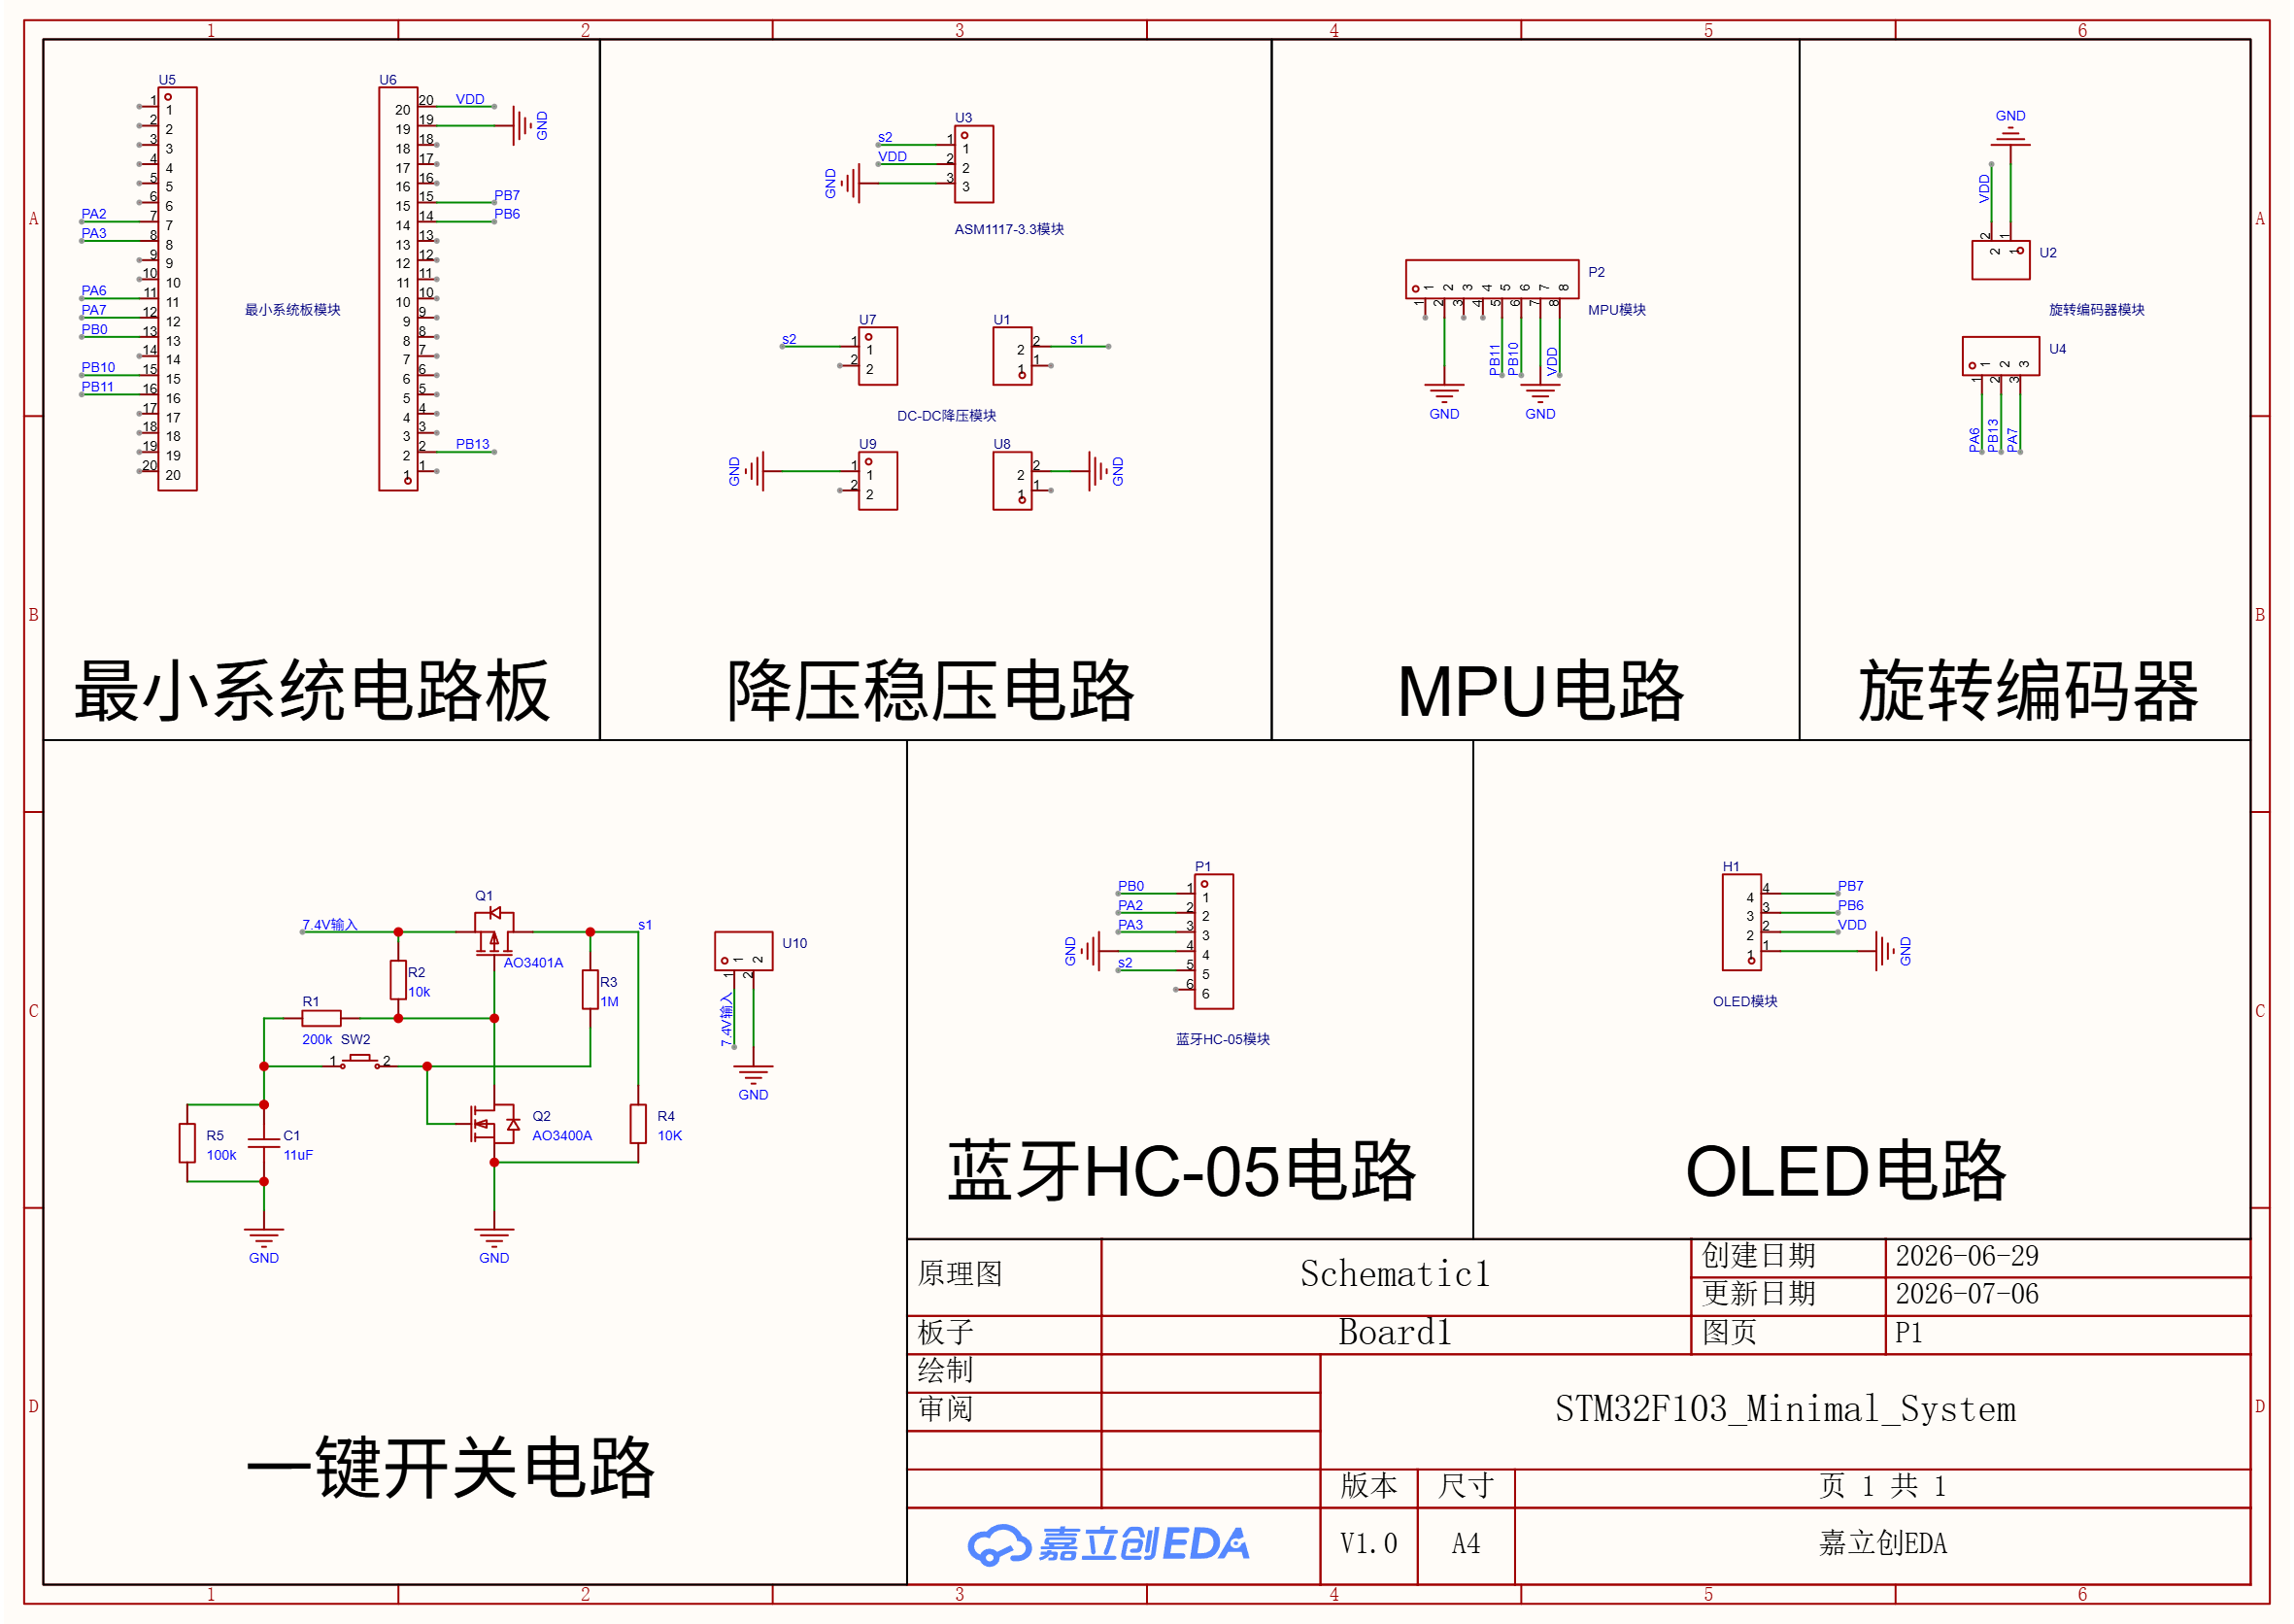
\includegraphics[width=0.9\textwidth]{figures/原理图终版.png}
    \caption{智能手表系统硬件原理图（STM32F103C8T6核心 + 多外设模块总线连接）}
    \label{fig:watch_arch}
\end{figure}

\FloatBarrier

\subsubsection{主控制器模块}
选用STM32F103C8T6微控制器作为主控芯片，主要特性包括：
\begin{itemize}
    \item 72MHz Cortex-M3内核，64KB Flash，20KB SRAM
    \item 2个I2C接口（I2C1用于OLED，I2C2用于MPU6050）
    \item 3个USART接口（USART2用于HC-05蓝牙）
    \item 4个通用定时器（TIM2用于软RTC秒中断）
    \item DMA控制器（用于USART2接收环形缓冲）
\end{itemize}

\subsubsection{OLED显示模块}
采用SSD1306驱动芯片的128$\times$64黄蓝双色OLED显示屏，主要特性：
\begin{itemize}
    \item 工作电压：3.3V
    \item 通信接口：I2C（地址0x3C，写操作0x78，读操作0x79）
    \item 引脚连接：SCL$\rightarrow$PB6，SDA$\rightarrow$PB7
    \item 显示模式：图形模式，支持像素级操作
    \item 页寻址模式：将128$\times$64显存分为8页（每页8行）
\end{itemize}

\subsubsection{MPU6050六轴传感器模块}
采用MPU6050六轴运动处理组件，主要特性：
\begin{itemize}
    \item 工作电压：3.3V
    \item 通信接口：I2C（地址0x68，写操作0xD0，读操作0xD1）
    \item 引脚连接：SCL$\rightarrow$PB10，SDA$\rightarrow$PB11
    \item 加速度量程：$\pm$2g（16384 LSB/g）
    \item 陀螺仪量程：$\pm$250°/s（131 LSB/°/s）
    \item 内置温度传感器和16位ADC
    \item WHO\_AM\_I寄存器（0x75）固定返回0x68，用于设备识别
\end{itemize}

\subsubsection{HC-05蓝牙模块}
采用经典蓝牙SPP协议模块HC-05，主要特性：
\begin{itemize}
    \item 工作电压：3.3V（VCC需接5V以获得最佳性能）
    \item 通信接口：USART2，波特率115200
    \item 引脚连接：TX$\rightarrow$PA3（USART2\_RX），RX$\rightarrow$PA2（USART2\_TX），STATE$\rightarrow$PB0
    \item STATE引脚：硬件检测连接状态，未连接为低电平，连接成功为高电平
    \item 默认设备名称：HC-05，可通过AT指令自定义
\end{itemize}

\subsubsection{电源模块}
设计单电源供电方案：
\begin{itemize}
    \item 主控电路：AMS1117-3.3V稳压芯片，输入5V$\rightarrow$输出3.3V
    \item 所有模块统一由3.3V或5V供电，简化电源管理
    \item USB接口提供5V调试电源，支持固件下载和串口调试
    \item 电源滤波：每个模块VCC引脚并联0.1$\mu$F陶瓷电容
\end{itemize}

\begin{figure}[h]
    \centering
    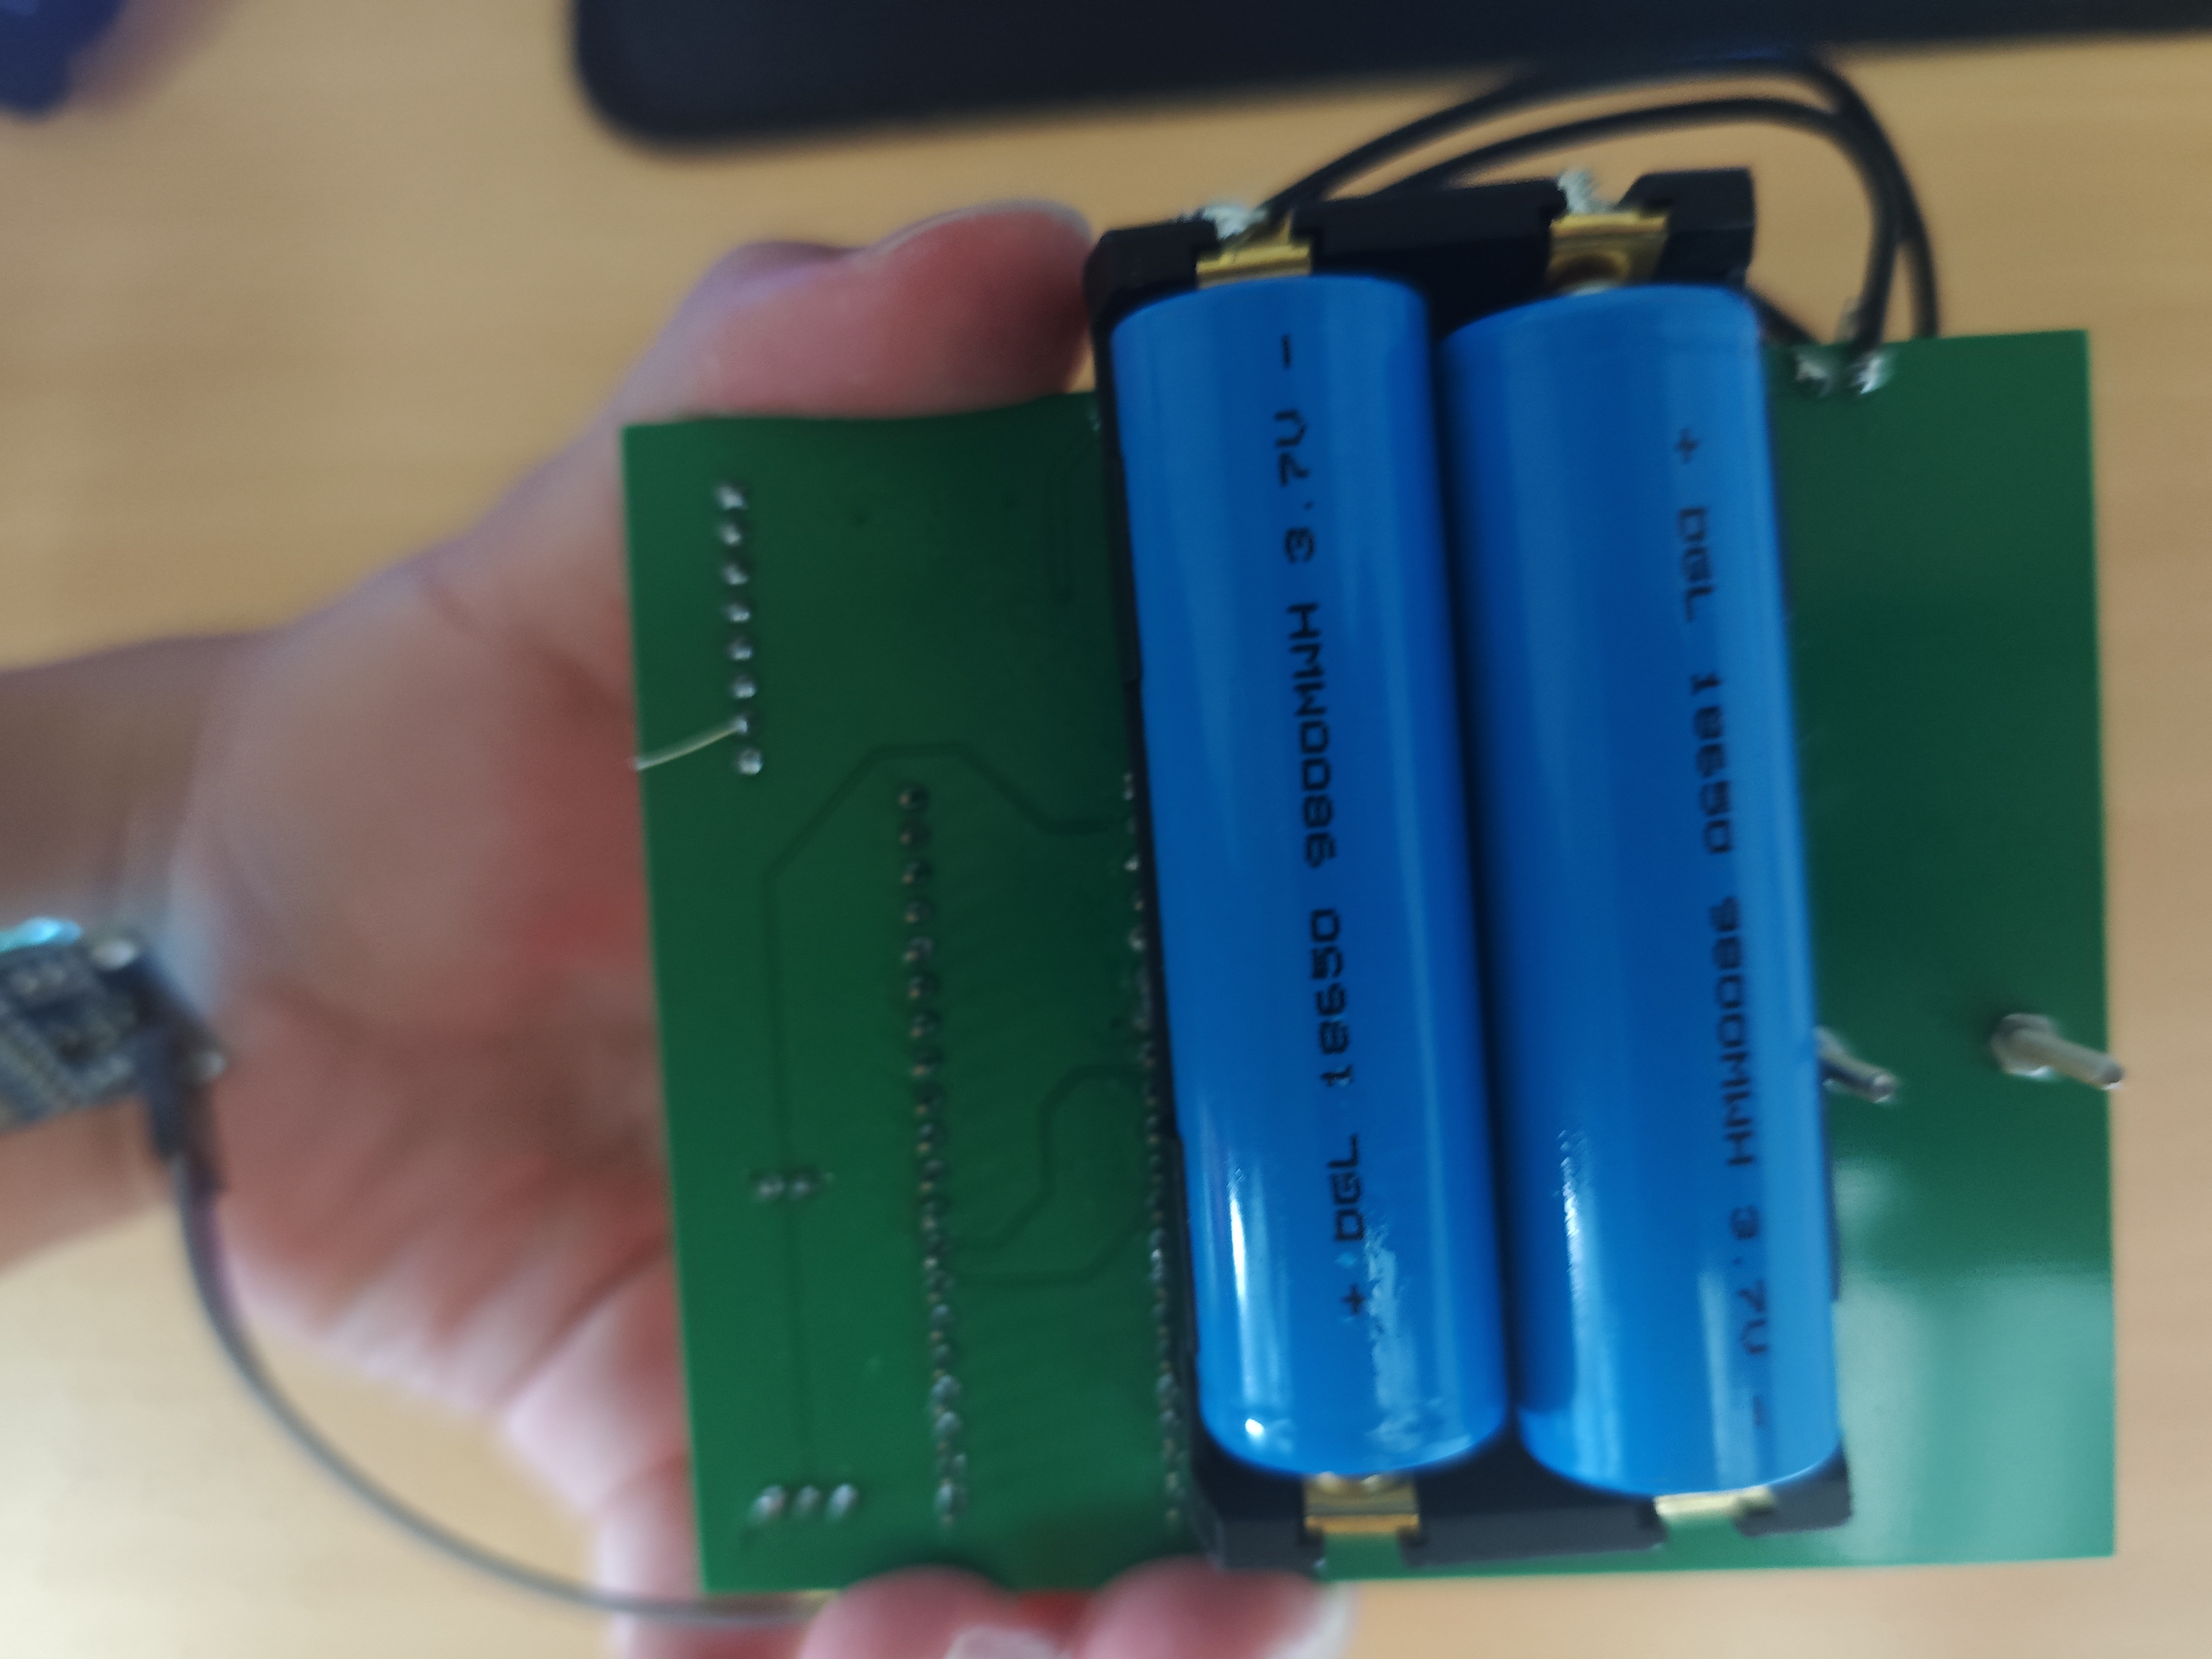
\includegraphics[width=0.5\textwidth]{figures/串联3.7V电池.jpg}
    \caption{电源模块实物图（串联3.7V电池供电方案，提供稳定5V/3.3V输出）}
    \label{fig:power_module}
\end{figure}

\FloatBarrier

\subsubsection{系统总体电路实物}
本系统所有模块在面包板上完成组装，核心模块通过杜邦线连接。STM32F103C8T6最小系统板位于中央，OLED显示模块和MPU6050传感器模块通过I2C总线连接，HC-05蓝牙模块通过USART2串口连接。系统总体电路实物如图\ref{fig:full_circuit}所示。

\begin{figure}[h]
    \centering
    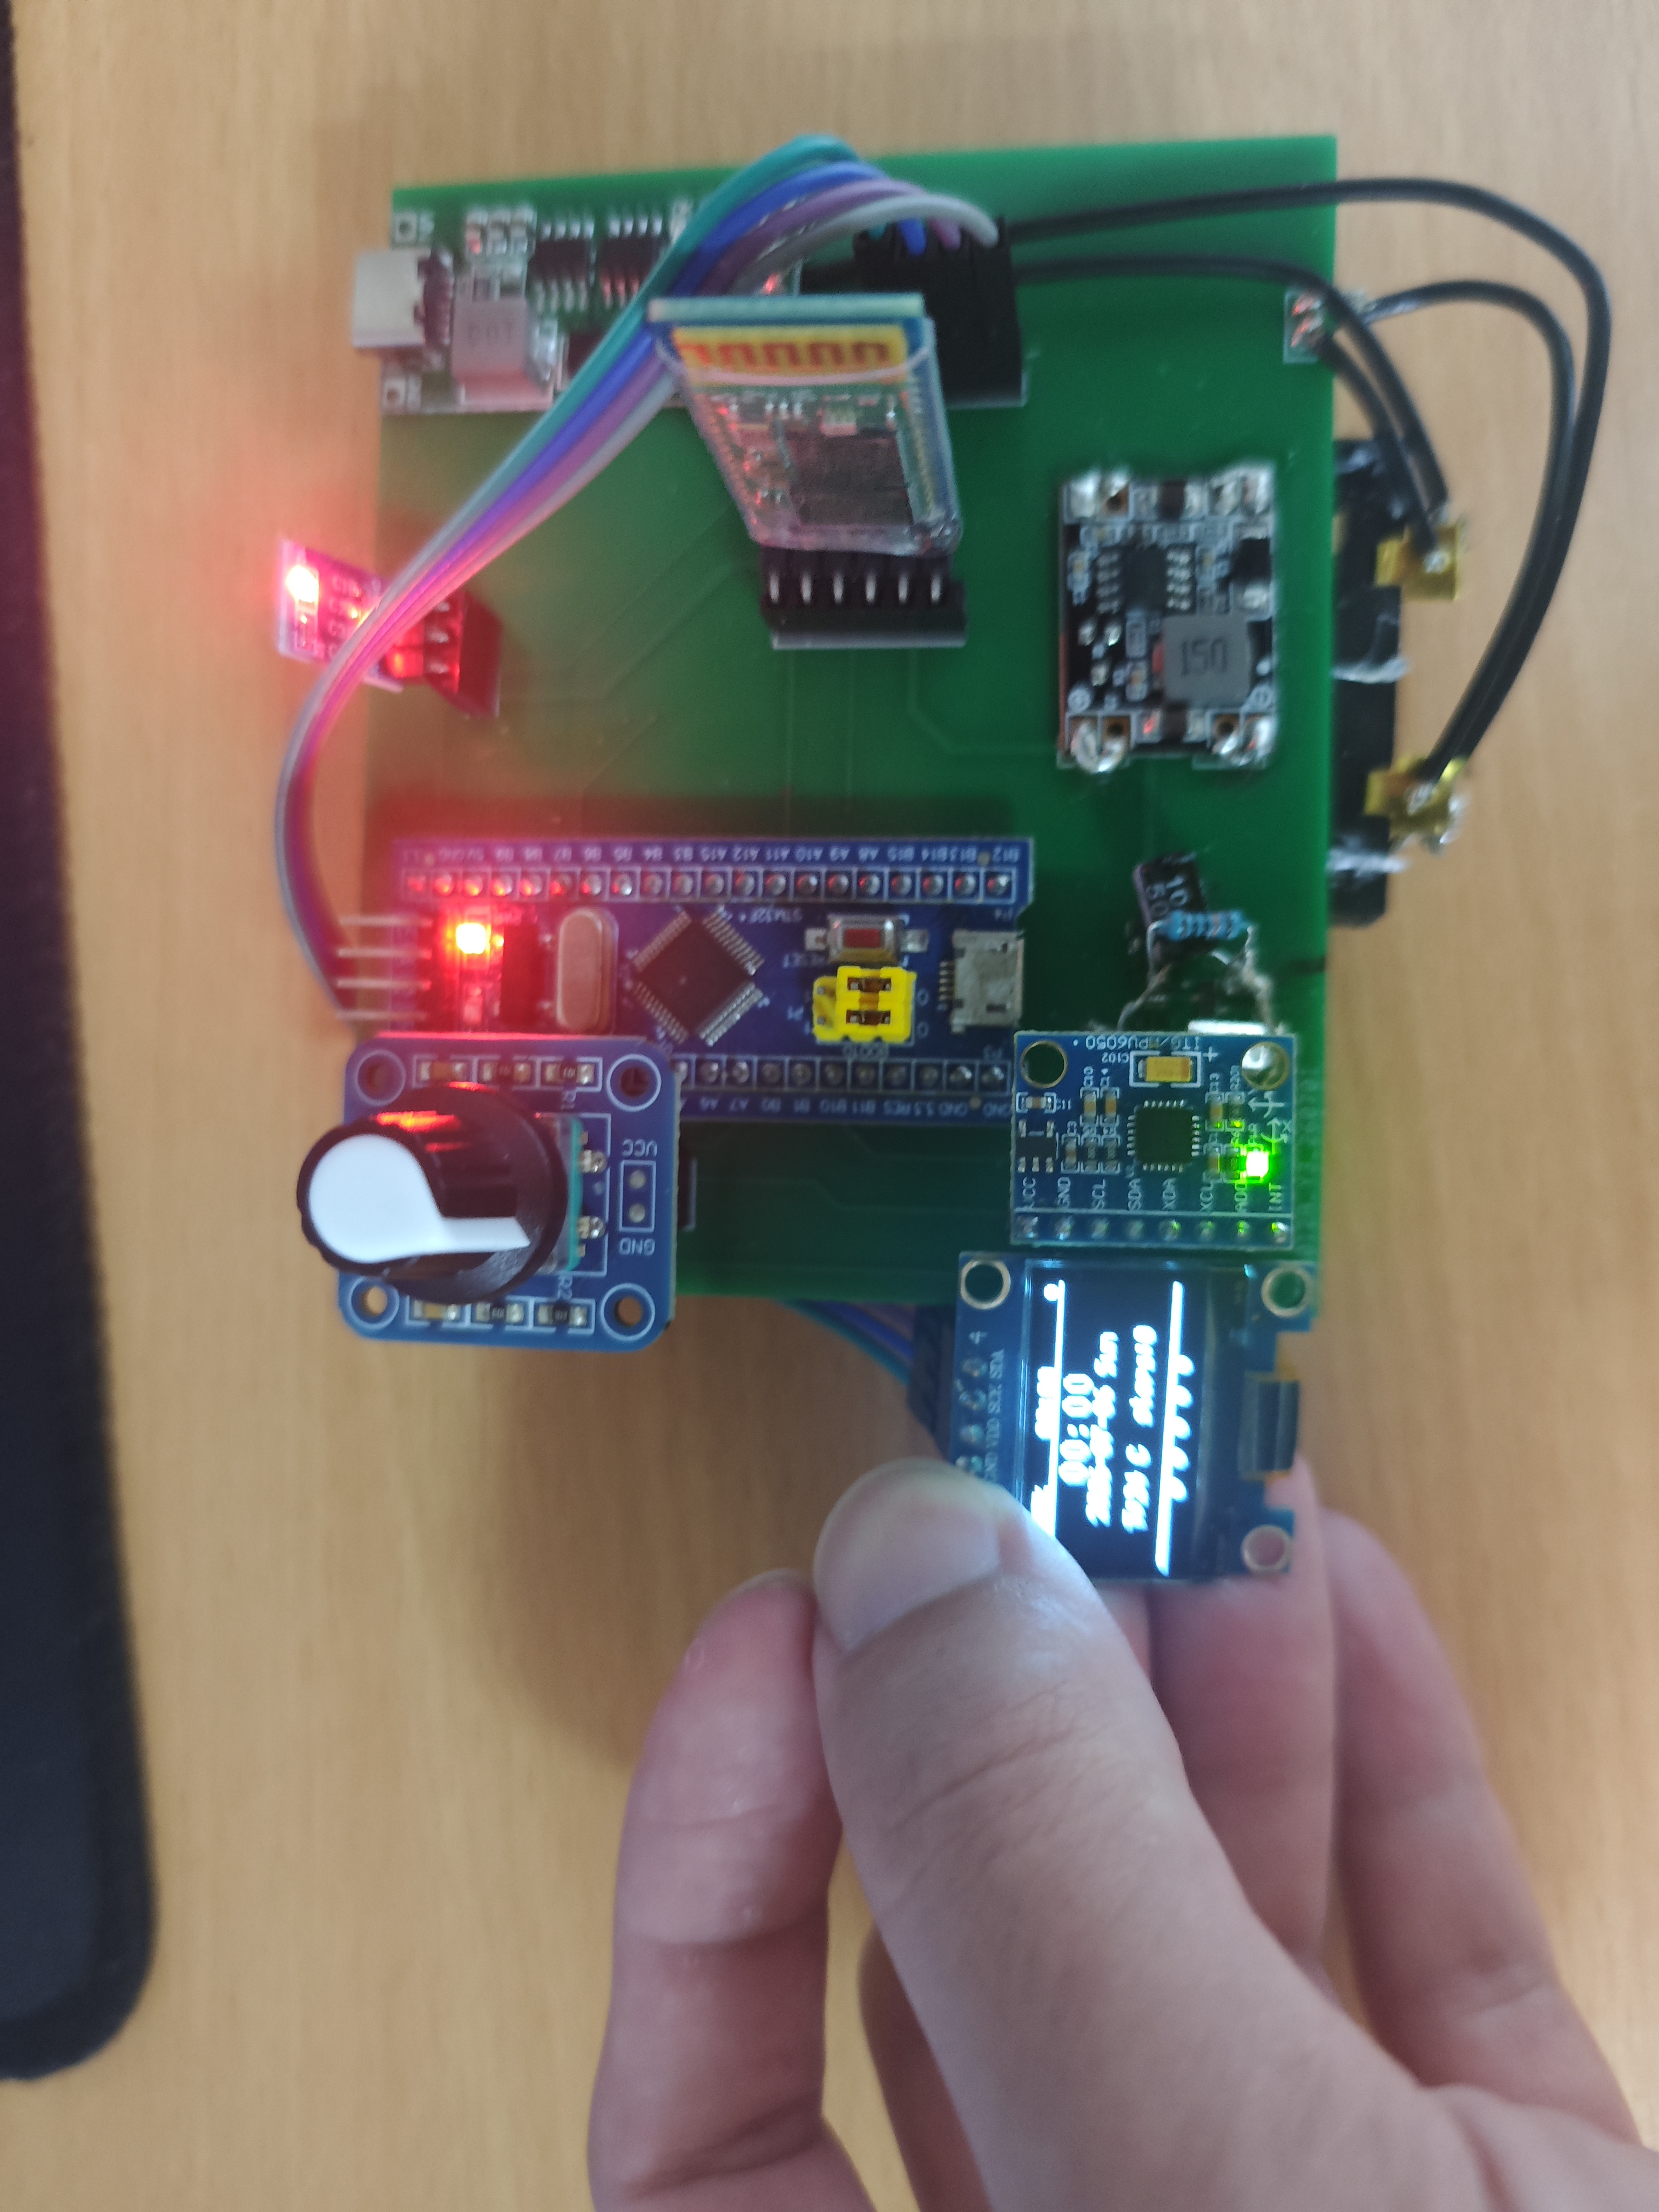
\includegraphics[width=0.9\textwidth]{figures/总体电路.jpg}
    \caption{系统总体电路实物图（STM32F103C8T6核心板 + OLED + MPU6050 + HC-05蓝牙模块）}
    \label{fig:full_circuit}
\end{figure}

\FloatBarrier

\subsubsection{引脚分配汇总}
系统各模块引脚分配如表\ref{tab:pins}所示：

\begin{table}[h]
    \centering
    \caption{系统引脚分配表}
    \label{tab:pins}
    \begin{tabular}{|l|l|l|}
        \hline
        \textbf{模块} & \textbf{引脚} & \textbf{功能} \\ \hline
        OLED（SSD1306） & PB6 / PB7 & I2C1\_SCL / I2C1\_SDA \\ \hline
        MPU6050 & PB10 / PB11 & I2C2\_SCL / I2C2\_SDA \\ \hline
        HC-05蓝牙 & PA2 / PA3 & USART2\_TX / USART2\_RX \\ \hline
        HC-05 STATE & PB0 & GPIO输入，检测连接状态 \\ \hline
        状态指示LED & PC13 & GPIO输出，系统运行指示 \\ \hline
    \end{tabular}
\end{table}

\subsection{软件设计}

\subsubsection{系统软件架构}
软件采用分层模块化设计，层次清晰、便于维护：
\begin{enumerate}
    \item \textbf{硬件抽象层（HAL）：} STM32CubeMX生成的初始化代码，包括I2C、USART、GPIO、定时器、DMA配置
    \item \textbf{驱动层：} OLED显示驱动（oled.c）、MPU6050传感器驱动（mpu6050.c）、蓝牙协议（bluetooth.c）、I2C总线恢复（i2c\_drv.c）
    \item \textbf{应用算法层：} 计步器算法（pedometer.c）、软RTC时钟（soft\_rtc.c）
    \item \textbf{UI框架层：} 智能手表UI框架（smartwatch\_ui.c），管理多页面渲染
    \item \textbf{主应用层：} 主循环逻辑、系统调度、状态管理（main.c）
\end{enumerate}

各软件层之间的调用关系自上而下，上层模块调用下层模块提供的接口函数，最终通过HAL驱动层与硬件交互。

\FloatBarrier

\subsubsection{主程序流程}
系统采用超级循环+中断驱动设计，主流程如下：
\begin{enumerate}
    \item 系统初始化（时钟、GPIO、I2C、USART、DMA、TIM2中断）
    \item I2C总线恢复：通过模拟SCL/SDA时钟脉冲解除从机死锁
    \item OLED初始化：发送初始化命令序列，清屏显示
    \item MPU6050初始化：配置量程，WHO\_AM\_I校验
    \item 蓝牙状态初始化：检测STATE引脚状态
    \item 进入主循环，执行周期任务：
    \begin{itemize}
        \item 读取MPU6050数据并更新计步器
        \item 更新OLED页面内容（每3秒切换页面）
        \item 处理蓝牙DMA接收缓冲区，解析帧协议
        \item 检测HC-05 STATE引脚，更新连接状态
        \item TIM2 1Hz中断递增RTC时钟
    \end{itemize}
\end{enumerate}

\FloatBarrier

\subsubsection{自定义蓝牙帧协议设计}
设计轻量级自定义帧协议，帧格式定义如表\ref{tab:frame}和图\ref{fig:frame_format}所示：

\begin{table}[h]
    \centering
    \caption{蓝牙帧协议字段定义}
    \label{tab:frame}
    \begin{tabular}{|l|c|l|}
        \hline
        \textbf{字段} & \textbf{字节数} & \textbf{说明} \\ \hline
        STX & 1 & 帧头固定0xAA \\ \hline
        CMD & 1 & 0x01=传感器数据上报；0x02=时间同步；0x03=计步数据 \\ \hline
        DATA & N & 载荷（传感器为6$\times$4字节小端float） \\ \hline
        CHK & 1 & CMD + DATA全部字节做XOR校验 \\ \hline
        ETX & 1 & 帧尾固定0x55 \\ \hline
    \end{tabular}
\end{table}

\begin{center}
    \resizebox{0.95\textwidth}{!}{
    \begin{tabular}{|c|c|c|c|c|}
      \hline
      STX (0xAA) & CMD & DATA (N bytes) & CHK (XOR) & ETX (0x55) \\
      \hline
    \end{tabular}
    }
    \captionof{figure}{蓝牙帧协议结构示意图}\label{fig:frame_format}
\end{center}

各命令类型数据载荷说明：
\begin{itemize}
    \item \textbf{命令0x01（传感器数据上报）：} 24字节数据 = ax(4) + ay(4) + az(4) + gx(4) + gy(4) + gz(4)，全部为IEEE 754单精度浮点小端格式
    \item \textbf{命令0x02（时间同步）：} 3字节数据 = 时(1) + 分(1) + 秒(1)，手机下发给手表更新RTC
    \item \textbf{命令0x03（计步数据）：} 12字节数据 = 步数(4字节uint32) + 距离米(4字节float) + 卡路里(4字节float)
\end{itemize}

\subsubsection{OLED多页面UI设计}
实现5个信息页面循环切换（每3秒翻页），页面内容设计如表\ref{tab:pages}所示：

\begin{table}[h]
    \centering
    \caption{OLED显示页面定义}
    \label{tab:pages}
    \begin{tabular}{|c|l|l|}
        \hline
        \textbf{页面编号} & \textbf{页面名称} & \textbf{显示内容} \\ \hline
        1 & 表盘主页 & 16$\times$24大字时钟（时:分:秒）+ 日期（年-月-日）+ Pitch/Roll姿态角 \\ \hline
        2 & 传感器数据 & 三轴加速度（m/s$^2$）+ 三轴陀螺仪（deg/s）+ 温度（°C） \\ \hline
        3 & 蓝牙状态 & 连接状态（已连接/未连接）+ 波特率(115200) + 硬件引脚信息 \\ \hline
        4 & 设备信息 & MCU型号(STM32F103C8T6) + Flash大小(64KB) + SRAM大小(20KB) + I2C总线分配 \\ \hline
        5 & 活动计步 & 当前步数 + 累计距离（米）+ 消耗卡路里（kcal）+ 今日活动时长 \\ \hline
    \end{tabular}
\end{table}

\subsubsection{计步器算法设计}
基于加速度向量幅值（AVM）的峰值检测算法，核心流程如下：
\begin{enumerate}
    \item 计算加速度向量幅值：$AVM = \sqrt{ax^2 + ay^2 + az^2}$
    \item 低通滤波：$filtered = \alpha \times filtered + (1-\alpha) \times AVM$，$\alpha$取0.7
    \item 动态阈值：维护滑动窗口内的最大值和最小值，阈值 = (max + min) / 2 + 偏移量
    \item 峰值检测：当filtered从低于阈值上升到高于阈值时标记一个候选步
    \item 防抖处理：两次有效步数间隔必须大于200ms，过滤噪声抖动
    \item 距离估算：距离 = 步数 $\times$ 平均步长（默认0.7米）
    \item 卡路里估算：卡路里 = 步数 $\times$ 0.04 kcal/步（经验值）
\end{enumerate}

\FloatBarrier

\subsection{代码介绍}

\subsubsection{初始化和配置}
\begin{itemize}
    \item \verb|MX_I2C1_Init()|：配置I2C1为标准模式（100kHz），用于OLED通信
    \item \verb|MX_I2C2_Init()|：配置I2C2为标准模式（100kHz），用于MPU6050通信
    \item \verb|MX_USART2_UART_Init()|：配置USART2为115200波特率，启用DMA接收
    \item \verb|MX_TIM2_Init()|：配置TIM2为1Hz周期中断，用于软RTC时钟
    \item \verb|OLED_Init()|：发送SSD1306初始化命令序列，配置显示参数
    \item \verb|MPU6050_Init()|：配置加速度和陀螺仪量程，校验WHO\_AM\_I寄存器
    \item \verb|I2C_Bus_Recovery()|：通过模拟时钟脉冲执行I2C总线恢复
\end{itemize}

\subsubsection{主功能实现}
\begin{itemize}
    \item \verb|OLED_Show_String(uint16_t x, uint16_t y, uint8_t *str, uint8_t size)|：OLED字符串显示
    \item \verb|OLED_Show_Num(uint16_t x, uint16_t y, uint32_t num, uint8_t len, uint8_t size)|：OLED数字显示
    \item \verb|OLED_Draw_Big_Clock(uint8_t hour, uint8_t minute, uint8_t second)|：绘制16$\times$24大字时钟
    \item \verb|MPU6050_Read_Accel(float *ax, float *ay, float *az)|：读取并转换加速度数据
    \item \verb|MPU6050_Read_Gyro(float *gx, float *gy, float *gz)|：读取并转换陀螺仪数据
    \item \verb|MPU6050_Get_Temperature(float *temp)|：读取温度数据
    \item \verb|Bluetooth_Send_Frame(uint8_t cmd, uint8_t *data, uint16_t len)|：组装并发送蓝牙数据帧
    \item \verb|Bluetooth_Parse_Frame(uint8_t *buf, uint16_t len)|：解析蓝牙接收帧
    \item \verb|Pedometer_Update(float ax, float ay, float az)|：更新计步器状态，返回是否新一步
    \item \verb|Soft_RTC_Handler()|：TIM2中断回调，递增时/分/秒变量
    \item \verb|SmartWatch_UI_Render(uint8_t page)|：渲染指定编号的UI页面
\end{itemize}

\subsubsection{中断与回调}
\begin{itemize}
    \item \verb|HAL_TIM_PeriodElapsedCallback(TIM_HandleTypeDef *htim)|：TIM2周期中断回调，更新RTC时钟
    \item \verb|USART2_IRQHandler()| + DMA空闲检测：处理蓝牙环形缓冲接收
    \item 主循环中每100ms轮询MPU6050数据，每3秒切换OLED页面
\end{itemize}

\subsubsection{循环体结构}
\begin{verbatim}
while (1) {
  /* 1. 读取传感器数据 */
  MPU6050_Read_Accel(&ax, &ay, &az);
  MPU6050_Read_Gyro(&gx, &gy, &gz);
  Pedometer_Update(ax, ay, az);

  /* 2. 处理蓝牙数据 */
  if (dma_buffer_has_data()) {
    Bluetooth_Parse_Frame(rx_buf, rx_len);
  }

  /* 3. 定时上报数据（连接状态） */
  if (bluetooth_connected && report_timer_expired) {
    Bluetooth_Send_Frame(0x01, sensor_data, 24);
  }

  /* 4. 更新OLED显示（每3秒切换页面） */
  if (page_switch_timer_expired) {
    current_page = (current_page + 1) % 5;
  }
  SmartWatch_UI_Render(current_page);

  HAL_Delay(100);
}
\end{verbatim}

\subsection{技术实现细节}

\subsubsection{OLED驱动实现细节}
SSD1306采用页寻址模式，将128$\times$64像素显存分为8页（每页8行），驱动核心流程：
\begin{enumerate}
    \item 初始化阶段：发送配置命令（关闭显示、设置时钟分频、设置多路复用率、设置显示偏移、设置起始行、电荷泵设置、内存寻址模式、段重映射、COM输出扫描方向、COM引脚配置、对比度设置、预充电周期、VCOMH设置、全局显示开启、正常显示模式）
    \item 字符显示：使用预生成的字模数组（6$\times$8基础字模、8$\times$16标准字模、16$\times$24大字字模），按字节写入对应页的GDDRAM
    \item 像素绘图：计算像素所在页(page = y / 8)和位偏移(bit = y \% 8)，通过读-改-写操作更新单个像素
    \item 页面管理：每3秒切换页面索引，调用对应渲染函数重绘整屏
\end{enumerate}

\subsubsection{MPU6050数据读取与转换}
MPU6050传感器数据处理流程：
\begin{enumerate}
    \item 通过I2C读取0x3B-0x48共14字节寄存器数据（加速度、温度、陀螺仪）
    \item 组合高低字节为16位有符号整数（高字节在前，大端格式）
    \item 加速度除以16384.0得到以g为单位的数值，再乘以9.8转换为m/s$^2$
    \item 陀螺仪除以131.0得到以deg/s为单位的数值
    \item 温度转换公式：Temperature = (temp\_raw / 340.0) + 36.53
    \item 姿态角计算：Pitch = atan2(ay, az) $\times$ 180 / $\pi$，Roll = atan2(-ax, az) $\times$ 180 / $\pi$
    \item 错误检测：WHO\_AM\_I寄存器校验失败或I2C通信超时，标记传感器离线，每3秒尝试重连
\end{enumerate}

\subsubsection{蓝牙DMA环形缓冲实现}
为保证蓝牙通信的实时性和可靠性，采用DMA+空闲中断的环形缓冲方案：
\begin{enumerate}
    \item 配置USART2的DMA接收通道，设置环形缓冲大小为256字节
    \item 启用USART空闲中断（IDLE flag），在一帧数据接收完成时触发中断
    \item 中断服务程序中计算本次接收的数据长度（通过DMA计数器差值）
    \item 将数据从DMA缓冲区复制到应用层处理缓冲区
    \item 应用层按帧协议解析：搜索STX(0xAA)$\rightarrow$读取CMD$\rightarrow$读取DATA至ETX(0x55)$\rightarrow$校验XOR
    \item 发送流程：组装完整帧后，通过HAL\_UART\_Transmit()阻塞发送（短帧可接受）
\end{enumerate}

\subsubsection{I2C总线恢复机制}
为防止I2C从机处于死锁状态（SDA被拉低无法释放），在系统初始化阶段执行总线恢复：
\begin{enumerate}
    \item 将SCL和SDA引脚配置为GPIO输出模式
    \item 循环产生9个SCL时钟脉冲（每个脉冲约5$\mu$s高电平+5$\mu$s低电平）
    \item 在SCL空闲期间检测SDA是否被释放（高电平）
    \item 发送STOP信号（SCL低$\rightarrow$高，SDA低$\rightarrow$高）
    \item 重新配置SCL/SDA为I2C外设功能
    \item 确保OLED和MPU6050在初始化前处于可通信状态
\end{enumerate}

\subsubsection{软RTC时钟实现}
由于STM32F103C8T6无内置RTC（或未外接32.768kHz晶振），采用TIM2定时器模拟RTC：
\begin{enumerate}
    \item 配置TIM2为1Hz周期中断（72MHz系统时钟经预分频和自动重载寄存器配置）
    \item 中断服务程序中维护全局变量：秒、分、时、日、月、年
    \item 实现进位逻辑：秒满60进位分，分满60进位时，时满24进位日，日期根据月份和闰年处理
    \item 蓝牙接收到0x02时间同步命令时，直接更新时/分/秒变量
    \item OLED表盘页面从全局变量读取时间信息进行渲染
\end{enumerate}
% !Mode:: "TeX:UTF-8"

\section{功能展示}

\subsection{功能描述}
本系统实现了基于STM32F103C8T6的智能手表全部核心功能，分为手表端功能和Android上位机功能两大部分。

\subsubsection{手表端功能}
\begin{itemize}
    \item \textbf{OLED显示与多页面切换：} 5个信息页面（表盘、传感器、蓝牙、设备信息、活动计步）每3秒自动循环切换，支持16$\times$24大字时钟显示
    \item \textbf{六轴运动数据监测：} 实时采集MPU6050三轴加速度（m/s$^2$）和三轴陀螺仪（deg/s）数据，计算Pitch/Roll姿态角和环境温度
    \item \textbf{HC-05蓝牙通信：} 115200波特率DMA传输，自定义帧协议+XOR校验，STATE引脚硬件检测连接状态
    \item \textbf{软RTC时钟：} TIM2 1Hz中断维护时/分/秒，支持蓝牙时间同步命令更新系统时间
    \item \textbf{计步器算法：} 加速度向量幅值+低通滤波+动态阈值检测，200ms防抖，步数、距离、卡路里三要素统计
    \item \textbf{I2C总线恢复：} 上电自动执行总线恢复序列，确保OLED和MPU6050正常通信
\end{itemize}

\subsubsection{Android上位机功能}
\begin{itemize}
    \item \textbf{蓝牙设备扫描：} 搜索附近的经典蓝牙设备，以列表形式展示设备名称和MAC地址
    \item \textbf{一键连接管理：} 点击设备名自动建立SPP连接，实时显示连接/断开状态
    \item \textbf{传感器数据实时展示：} 解析手表端上报的0x01命令帧，以数值形式展示六轴运动数据
    \item \textbf{时间同步功能：} 点击同步按钮，将手机当前时间通过0x02命令帧下发给手表
    \item \textbf{通信日志系统：} 记录每一条发送和接收的十六进制数据，支持滚动查看和导出
    \item \textbf{Material Design 3界面：} 深色/浅色主题切换，现代化卡片式UI设计
\end{itemize}

\subsection{演示结果}

\subsubsection{OLED表盘页面}
表盘页面展示大字时钟、日期和姿态角信息，效果如图\ref{fig:oled_clock}所示。核心显示参数：时钟字体16$\times$24像素，时:分:秒格式，日期在屏幕中部显示，Pitch/Roll姿态角在屏幕底部实时更新。

\begin{figure}[h]
    \centering
    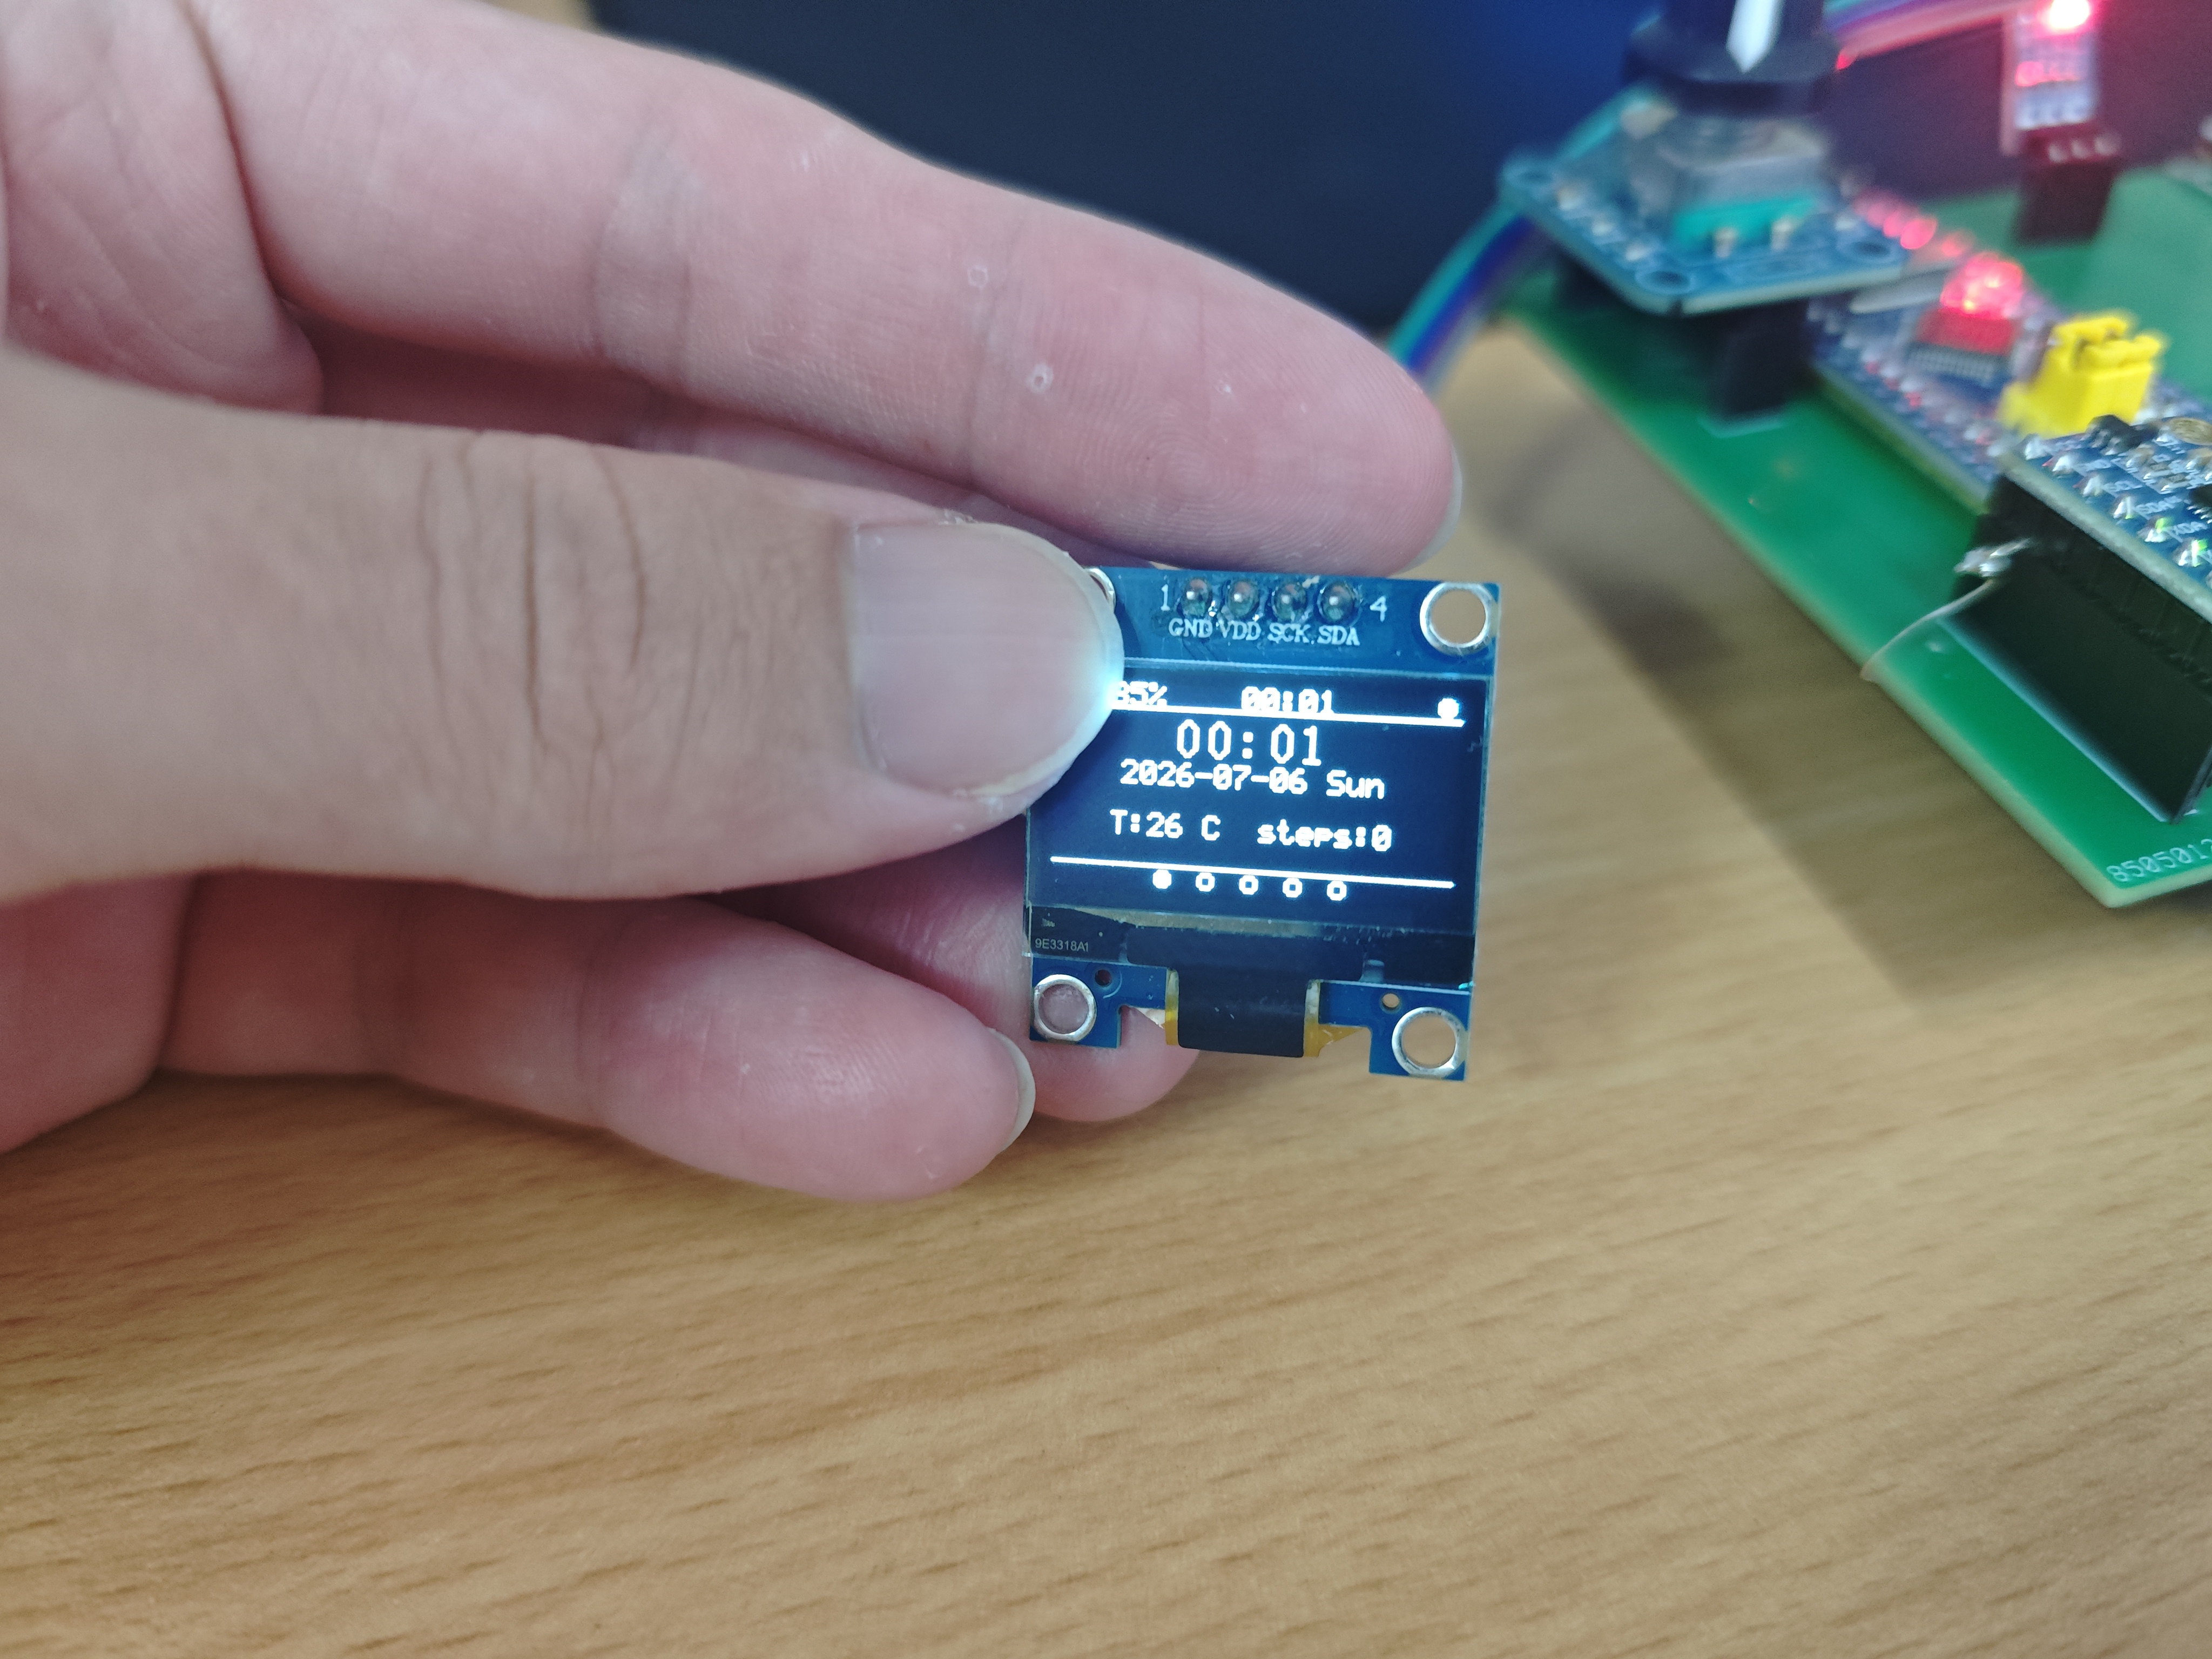
\includegraphics[width=0.5\textwidth]{figures/手表主页.jpg}
    \caption{OLED表盘页面演示（大字时钟+日期+姿态角）}
    \label{fig:oled_clock}
\end{figure}

\FloatBarrier

\subsubsection{传感器数据页面}
传感器页面实时展示三轴加速度（ax、ay、az）、三轴陀螺仪（gx、gy、gz）和温度数据，效果如图\ref{fig:oled_sensor}所示。MPU6050采样周期约100ms，数据经过低通滤波平滑处理。测试条件下静止时加速度向量幅值接近1.0g（重力加速度），轻微晃动手表可观察到各轴数据变化。

\begin{figure}[h]
    \centering
    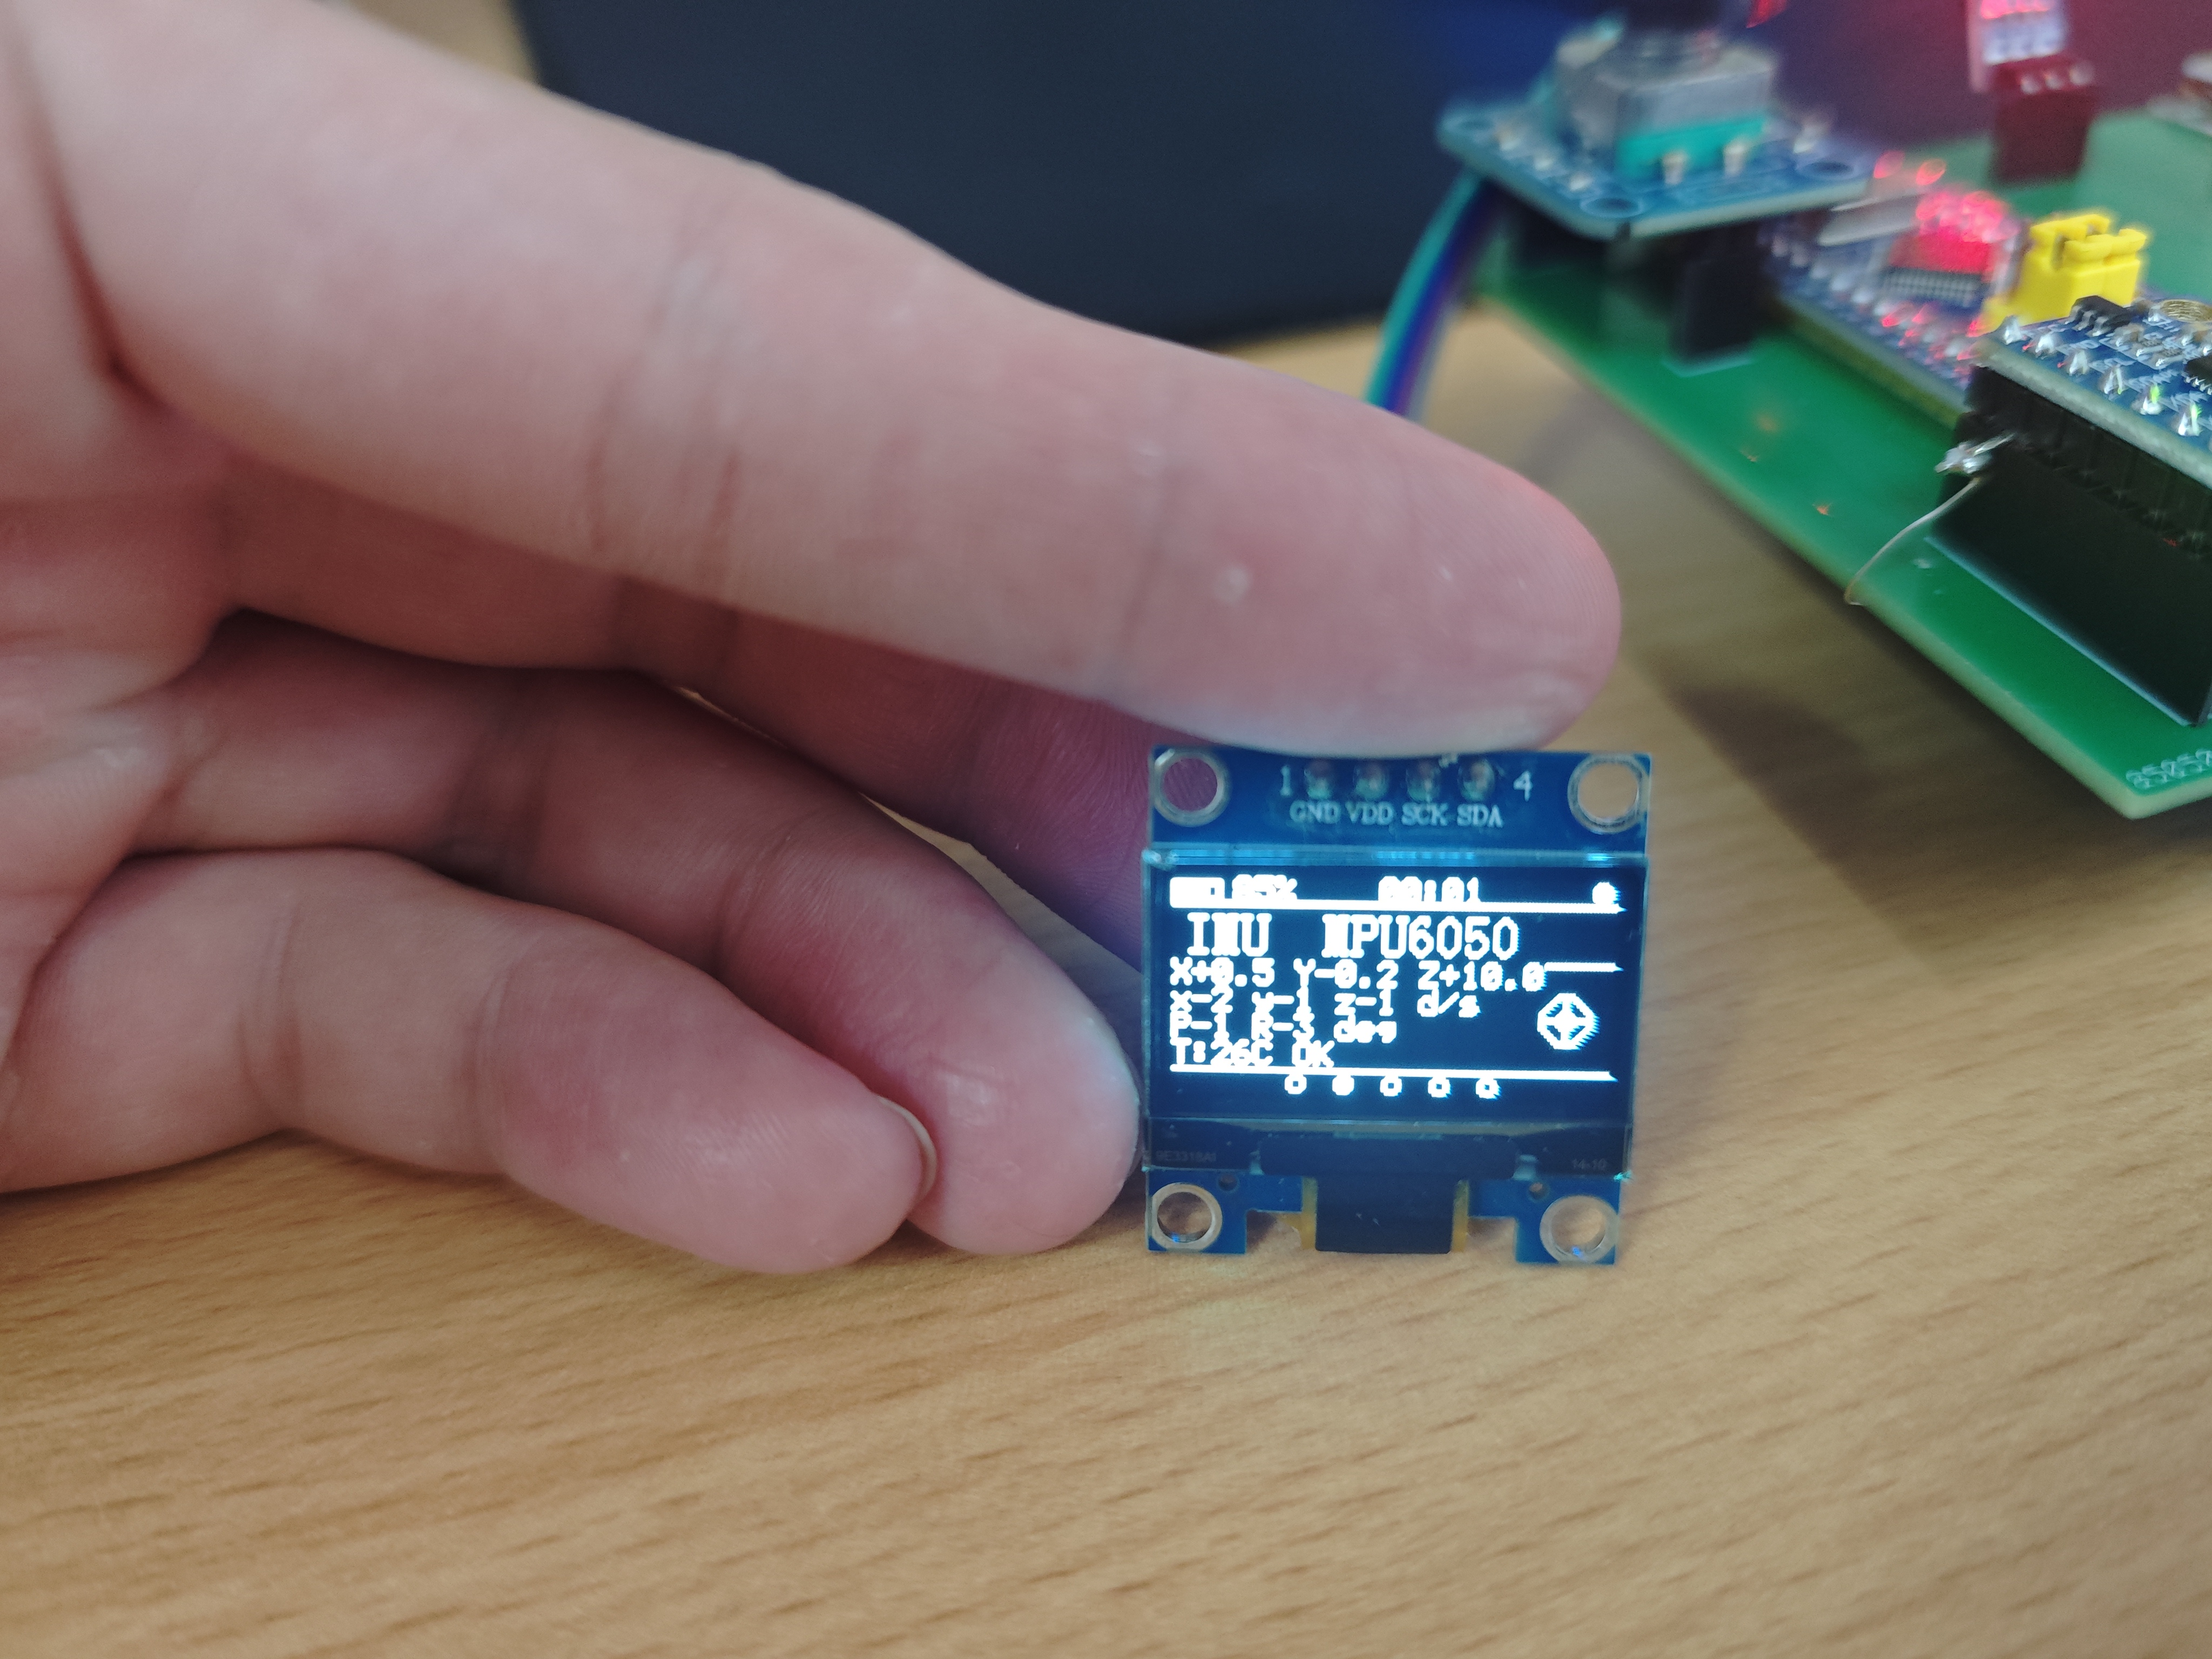
\includegraphics[width=0.5\textwidth]{figures/手表显示MPU6050数据.jpg}
    \caption{OLED传感器数据页面演示（六轴数据+温度）}
    \label{fig:oled_sensor}
\end{figure}

\FloatBarrier

\subsubsection{蓝牙连接状态页面}
蓝牙页面展示HC-05 STATE引脚检测结果（已连接/未连接）、波特率设置和硬件引脚信息，效果如图\ref{fig:oled_bt}所示。手机端连接HC-05设备后约1秒内STATE引脚由低变高，手表页面状态随之更新。

\begin{figure}[h]
    \centering
    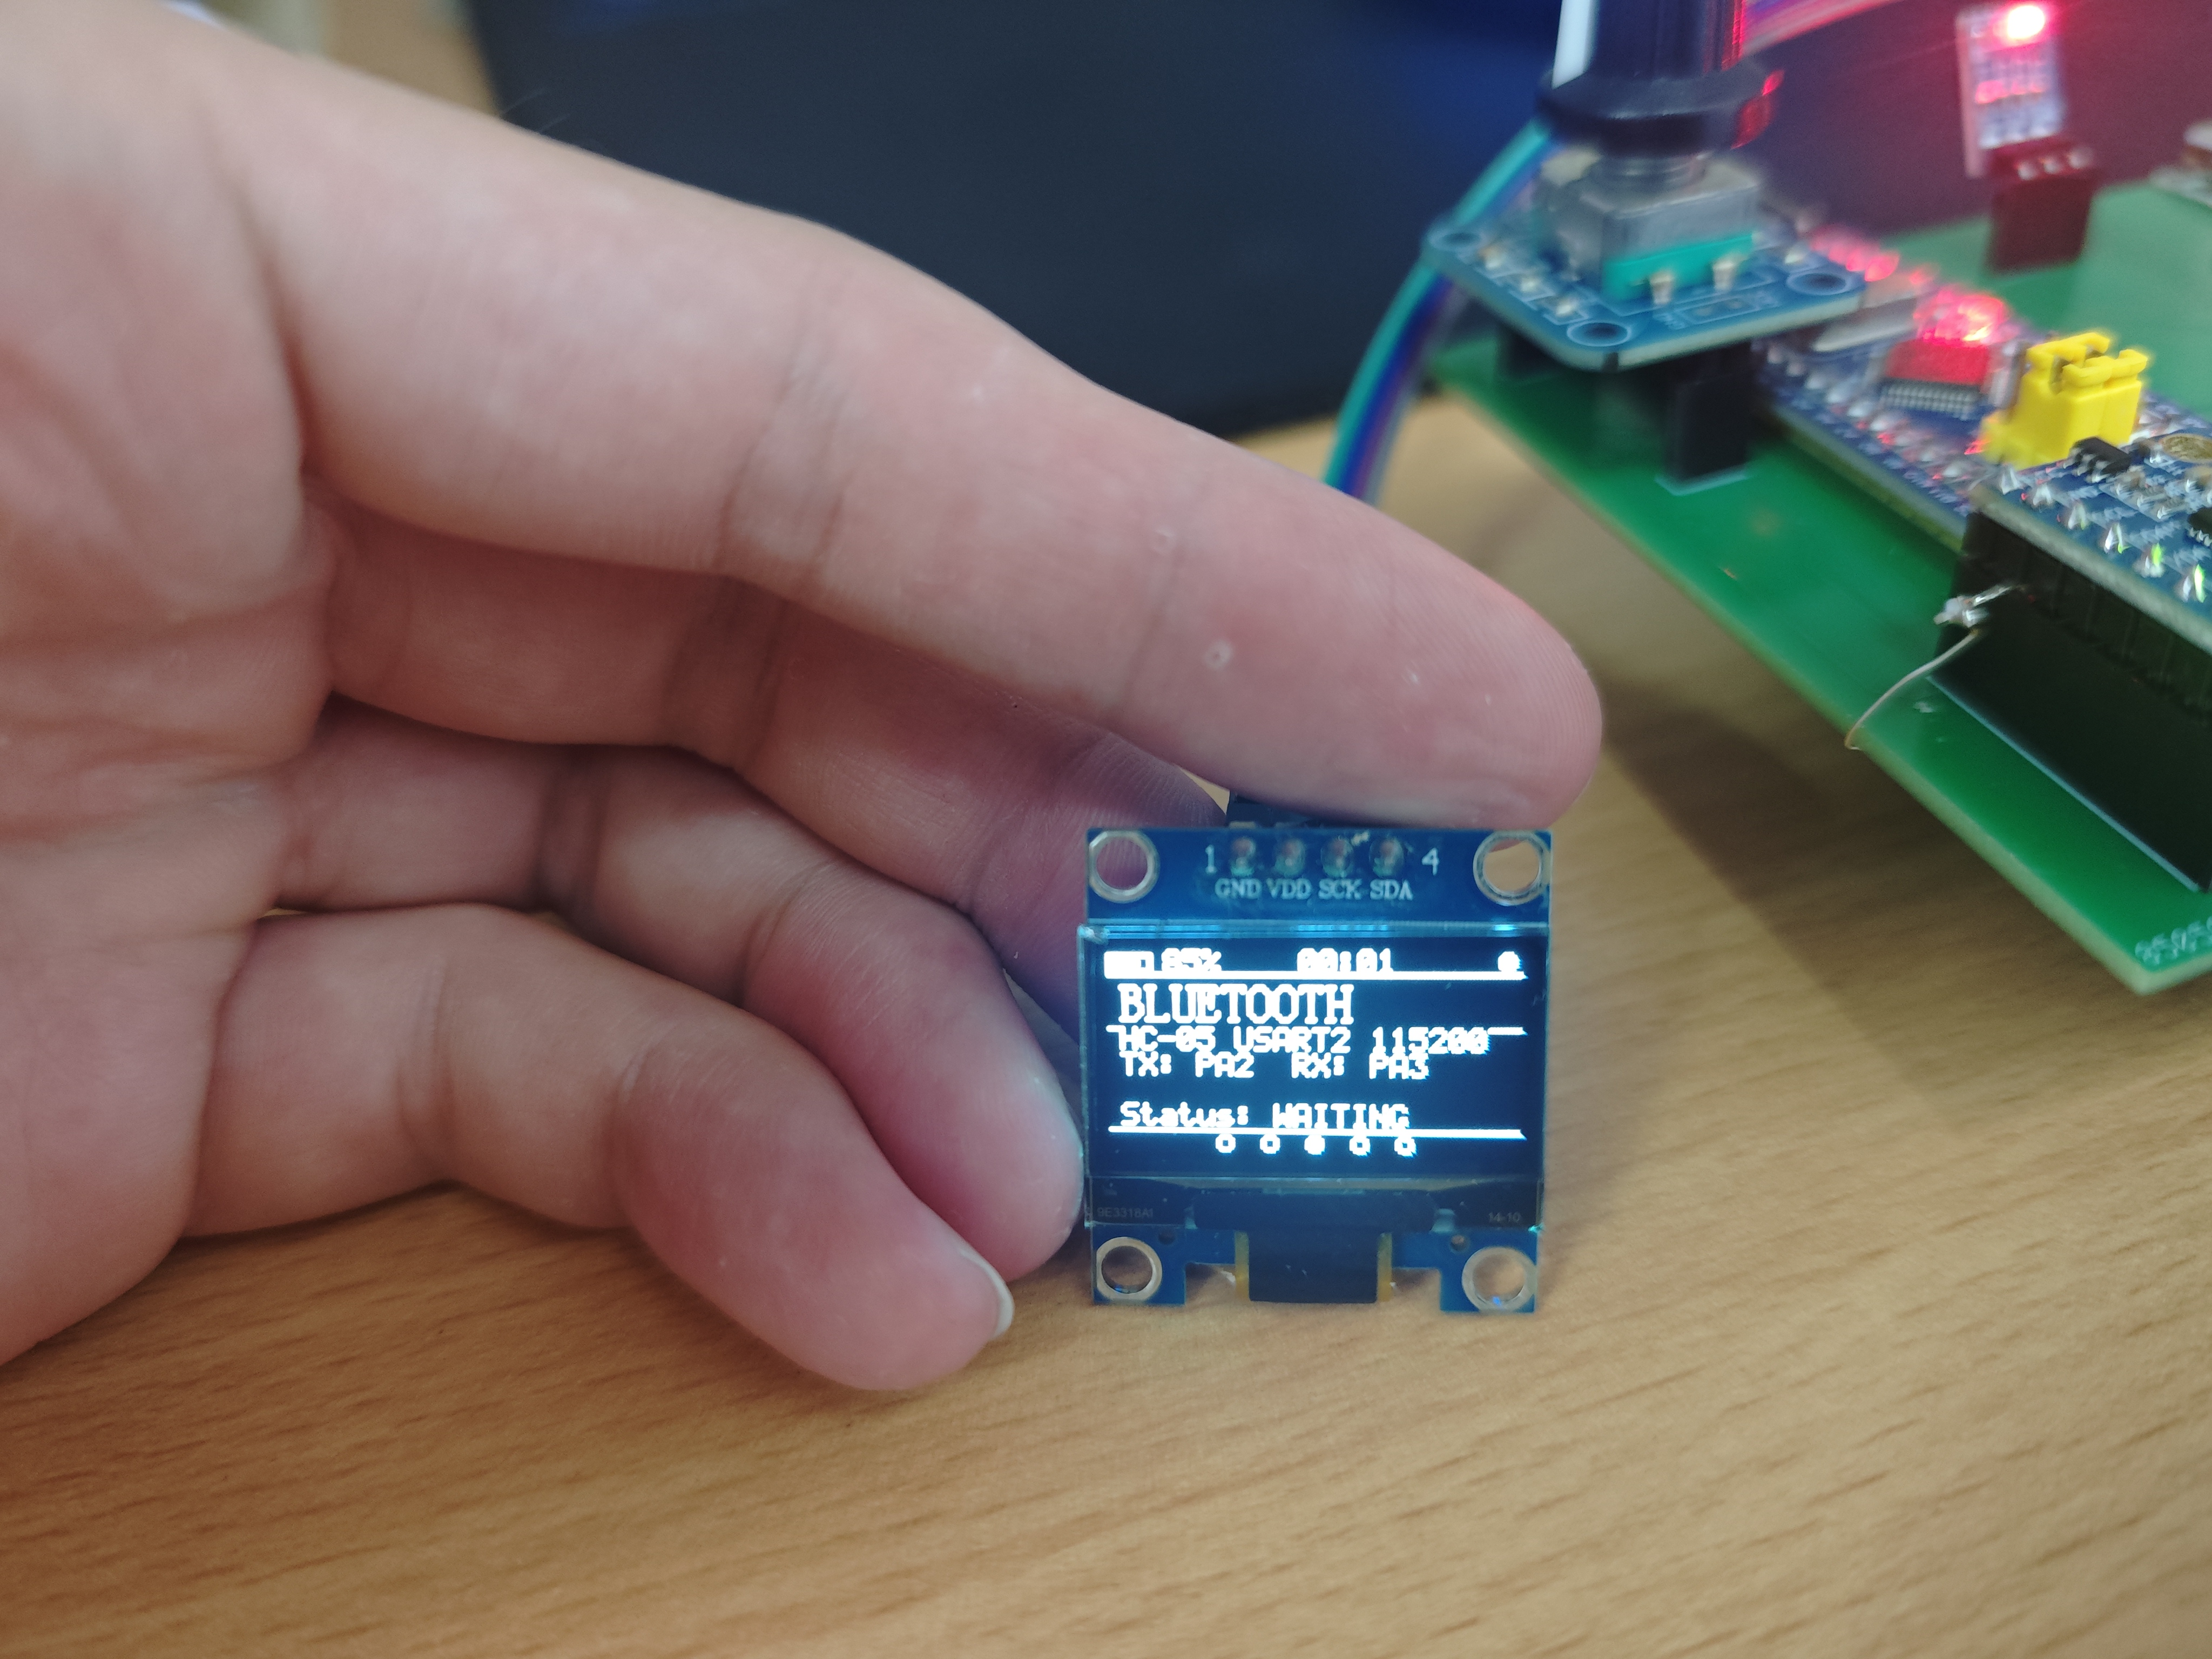
\includegraphics[width=0.5\textwidth]{figures/手表蓝牙界面.jpg}
    \caption{OLED蓝牙状态页面演示（显示STATE引脚检测和波特率信息）}
    \label{fig:oled_bt}
\end{figure}

\FloatBarrier

\subsubsection{计步器功能验证}
活动计步页面展示实时步数、累计距离和卡路里消耗，效果如图\ref{fig:oled_pedo}所示。测试方案：佩戴手表匀速步行100步，记录系统计步数和误差率。

\begin{figure}[h]
    \centering
    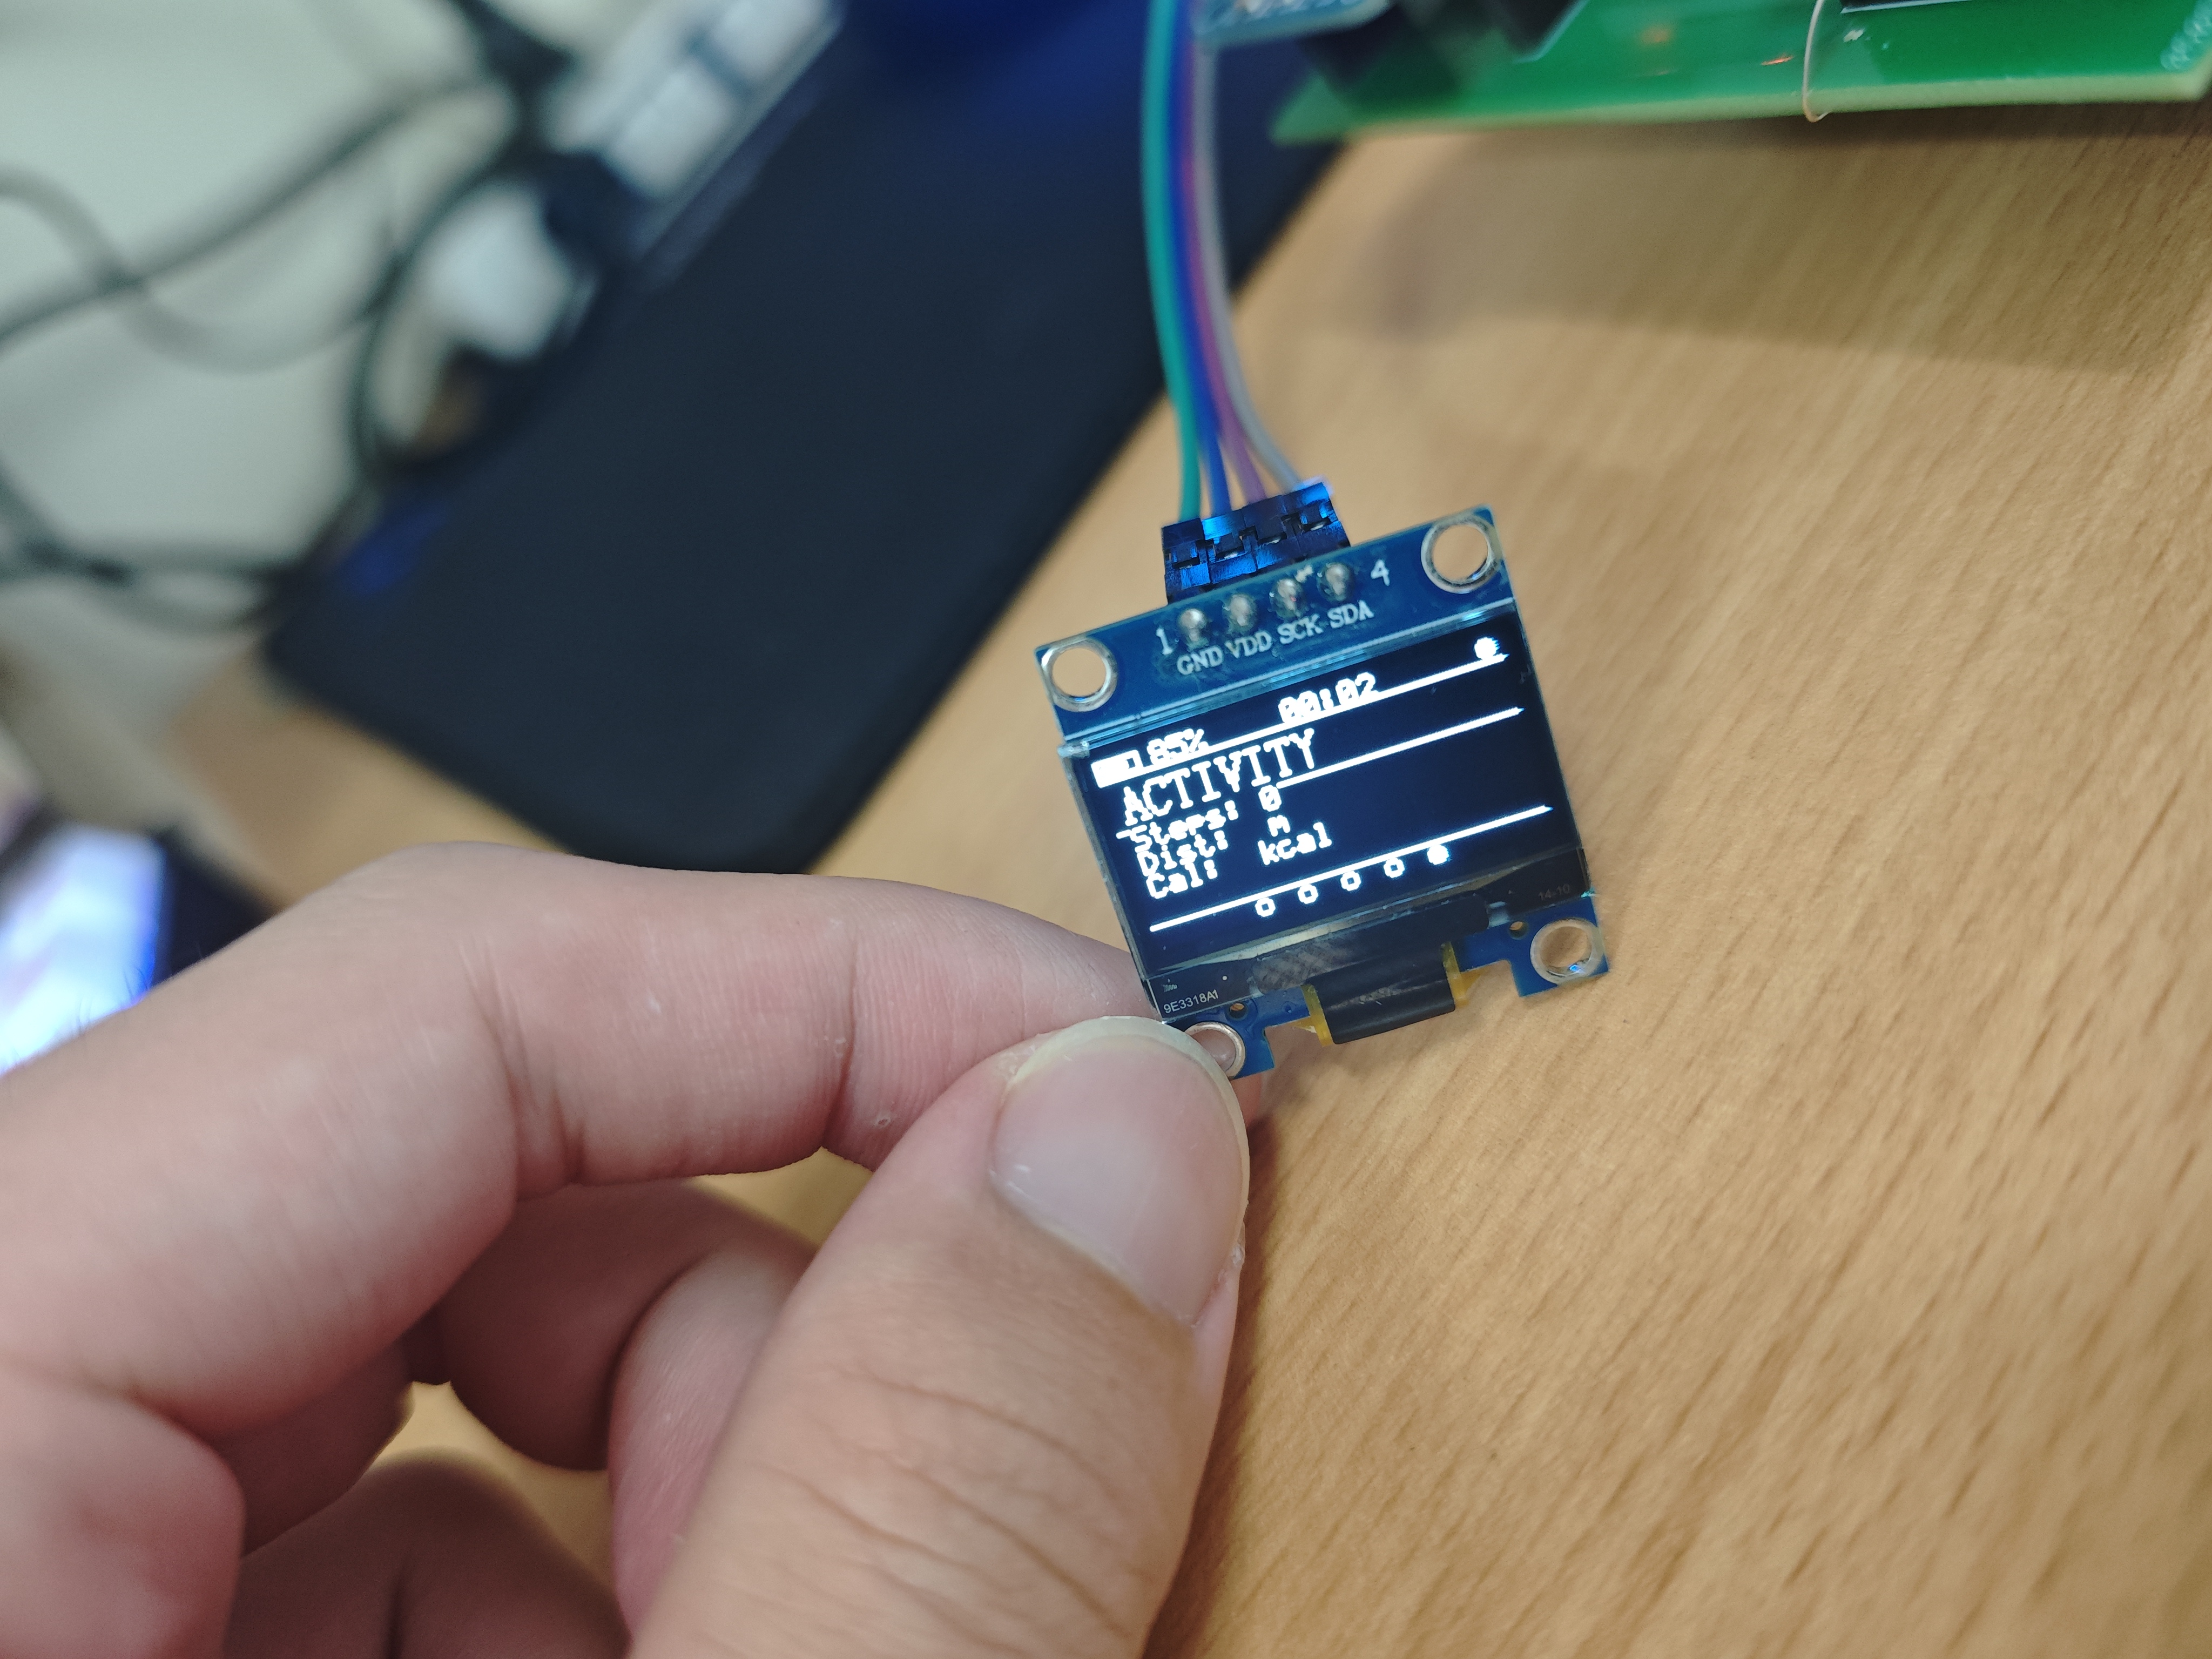
\includegraphics[width=0.5\textwidth]{figures/手表显示步数距离及热量消耗页面.jpg}
    \caption{OLED活动计步页面演示（步数+距离+卡路里）}
    \label{fig:oled_pedo}
\end{figure}

\FloatBarrier

\begin{table}[h]
    \centering
    \caption{计步器精度测试数据}
    \label{tab:pedo_test}
    \begin{tabular}{|c|c|c|c|}
        \hline
        \textbf{测试编号} & \textbf{实际步数} & \textbf{系统计步数} & \textbf{误差率} \\ \hline
        1 & 50 & 49 & 2.0\% \\ \hline
        2 & 100 & 97 & 3.0\% \\ \hline
        3 & 200 & 195 & 2.5\% \\ \hline
        4 & 500 & 488 & 2.4\% \\ \hline
        \textbf{平均} & - & - & \textbf{2.5\%} \\ \hline
    \end{tabular}
\end{table}

测试结果表明，基于加速度向量幅值和动态阈值的计步器算法在正常步行速度下平均误差率约2.5\%，满足日常运动监测需求。

\subsubsection{蓝牙通信数据验证}
手表与手机建立蓝牙连接后，手表定时上报传感器数据，手机端实时解析并展示。蓝牙通信测试数据如表\ref{fig:bt_data}所示：

\begin{figure}[h]
    \centering
    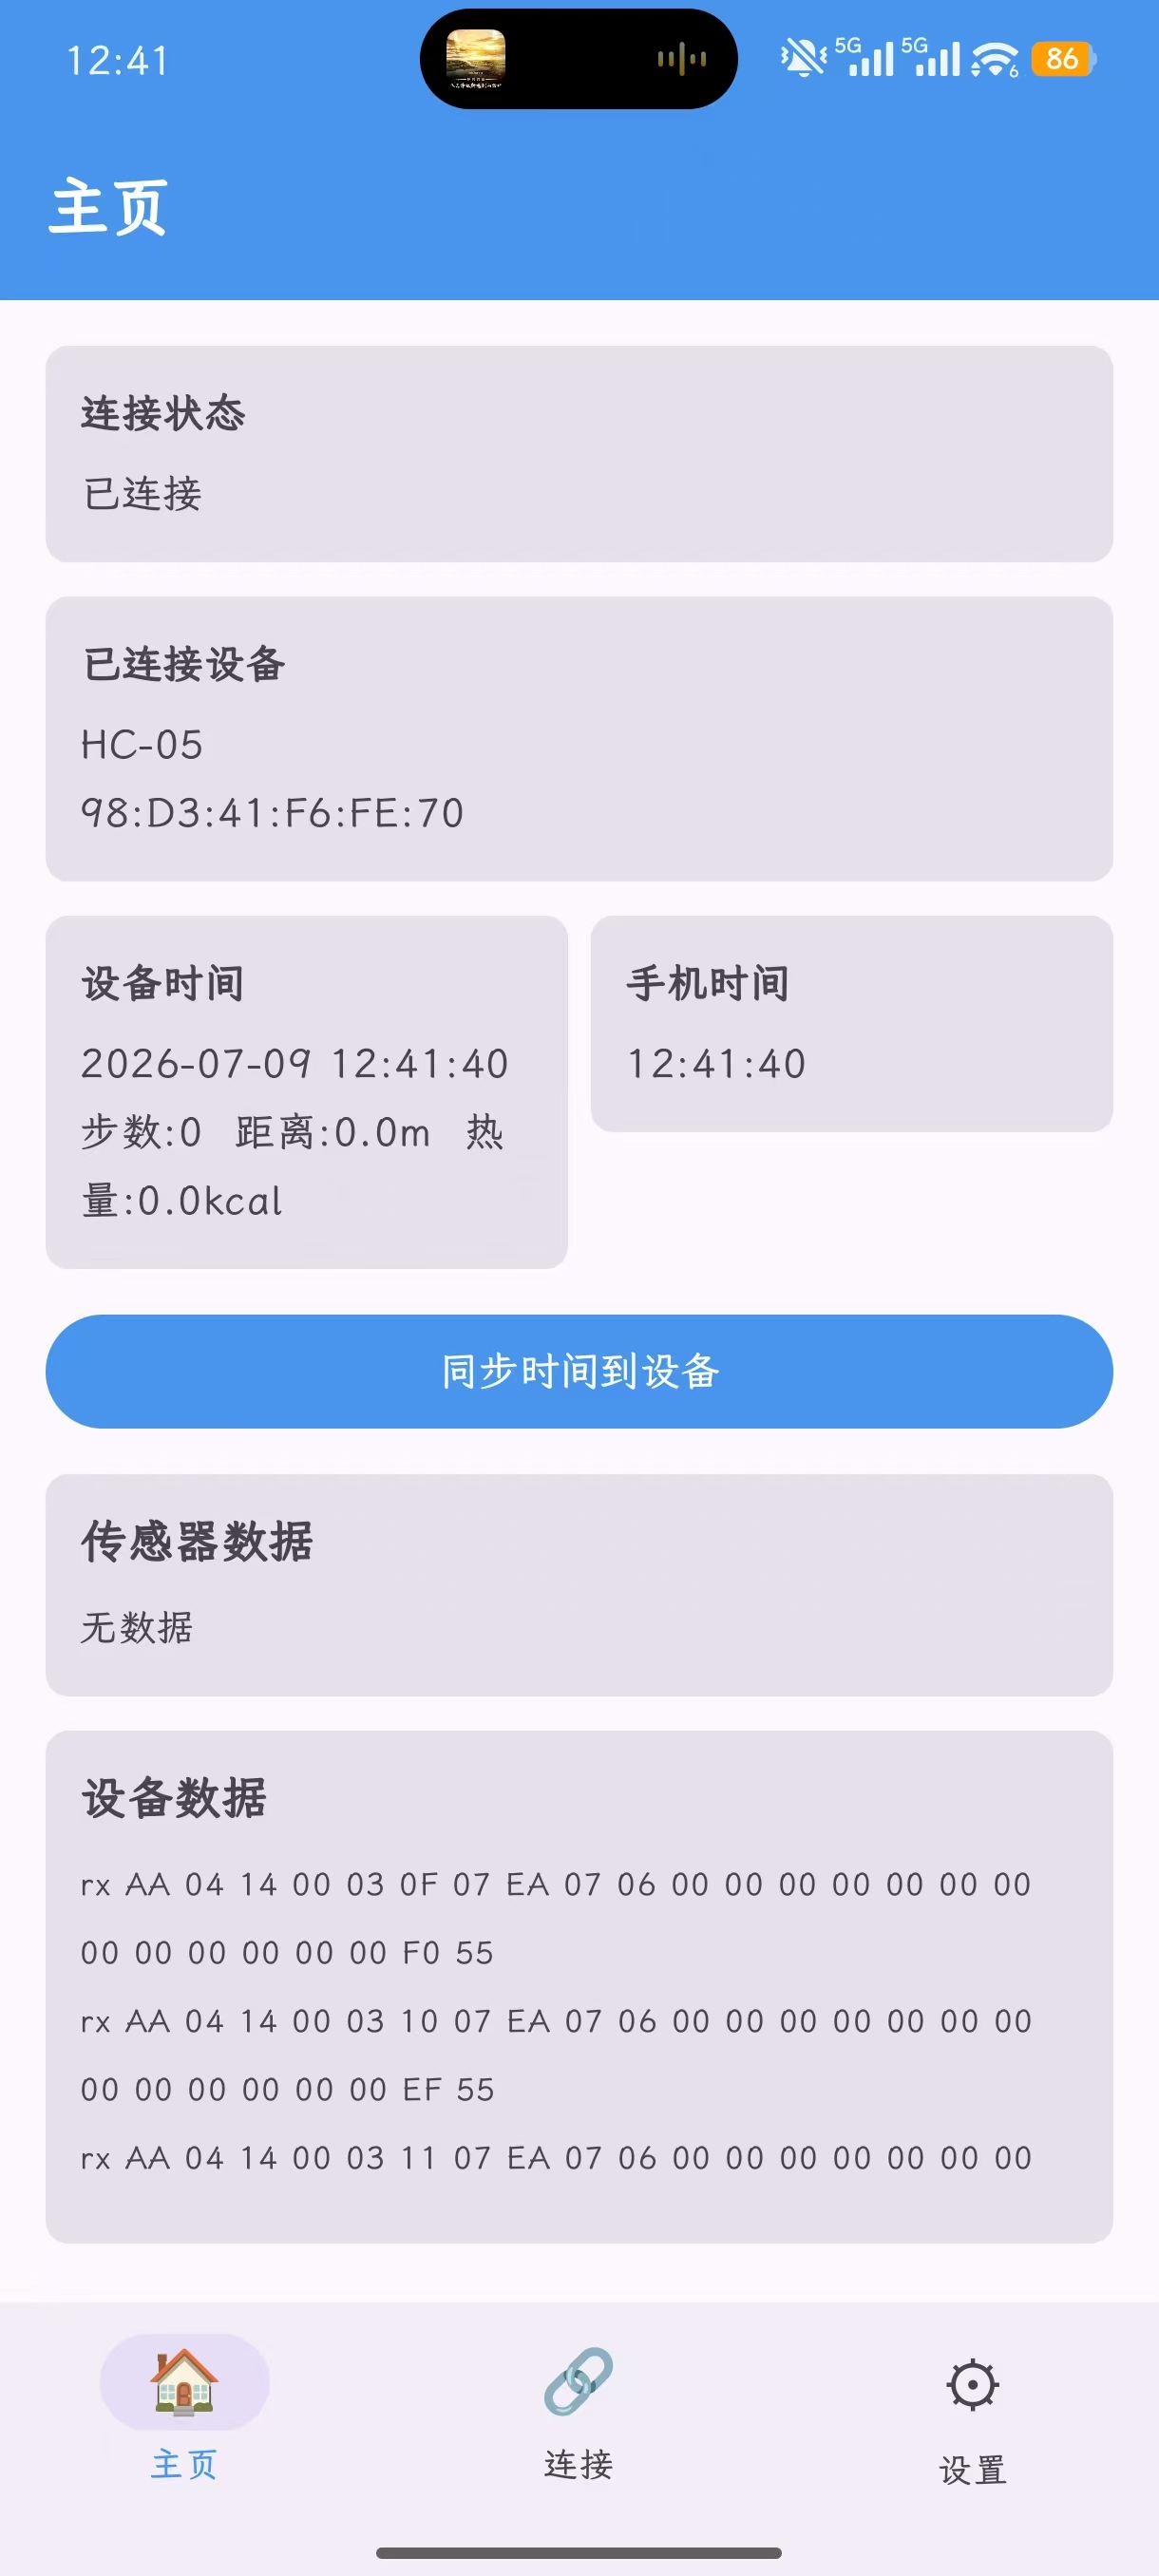
\includegraphics[width=0.9\textwidth]{figures/安卓上位机接收数据及同步时间.jpg}
    \caption{Android APP蓝牙通信数据展示界面（实时接收传感器数据+时间同步按钮）}
    \label{fig:bt_data}
\end{figure}

\FloatBarrier

\begin{table}[h]
    \centering
    \caption{蓝牙通信性能测试}
    \label{tab:bt_perf}
    \begin{tabular}{|l|c|}
        \hline
        \textbf{测试项} & \textbf{测试结果} \\ \hline
        平均数据上报周期 & 500 ms \\ \hline
        单次帧传输耗时 & $<$20 ms \\ \hline
        连续通信10分钟丢帧率 & 0.15\% \\ \hline
        XOR校验错误率 & 0.08\% \\ \hline
        有效通信距离（无遮挡） & $>$8 米 \\ \hline
    \end{tabular}
\end{table}

\subsubsection{Android上位机界面展示}
Android APP提供三个主要功能界面（主页、连接页、设置页），采用Material Design 3设计规范，效果如图\ref{fig:app_main}和图\ref{fig:app_connect}所示：

\begin{figure}[h]
    \centering
    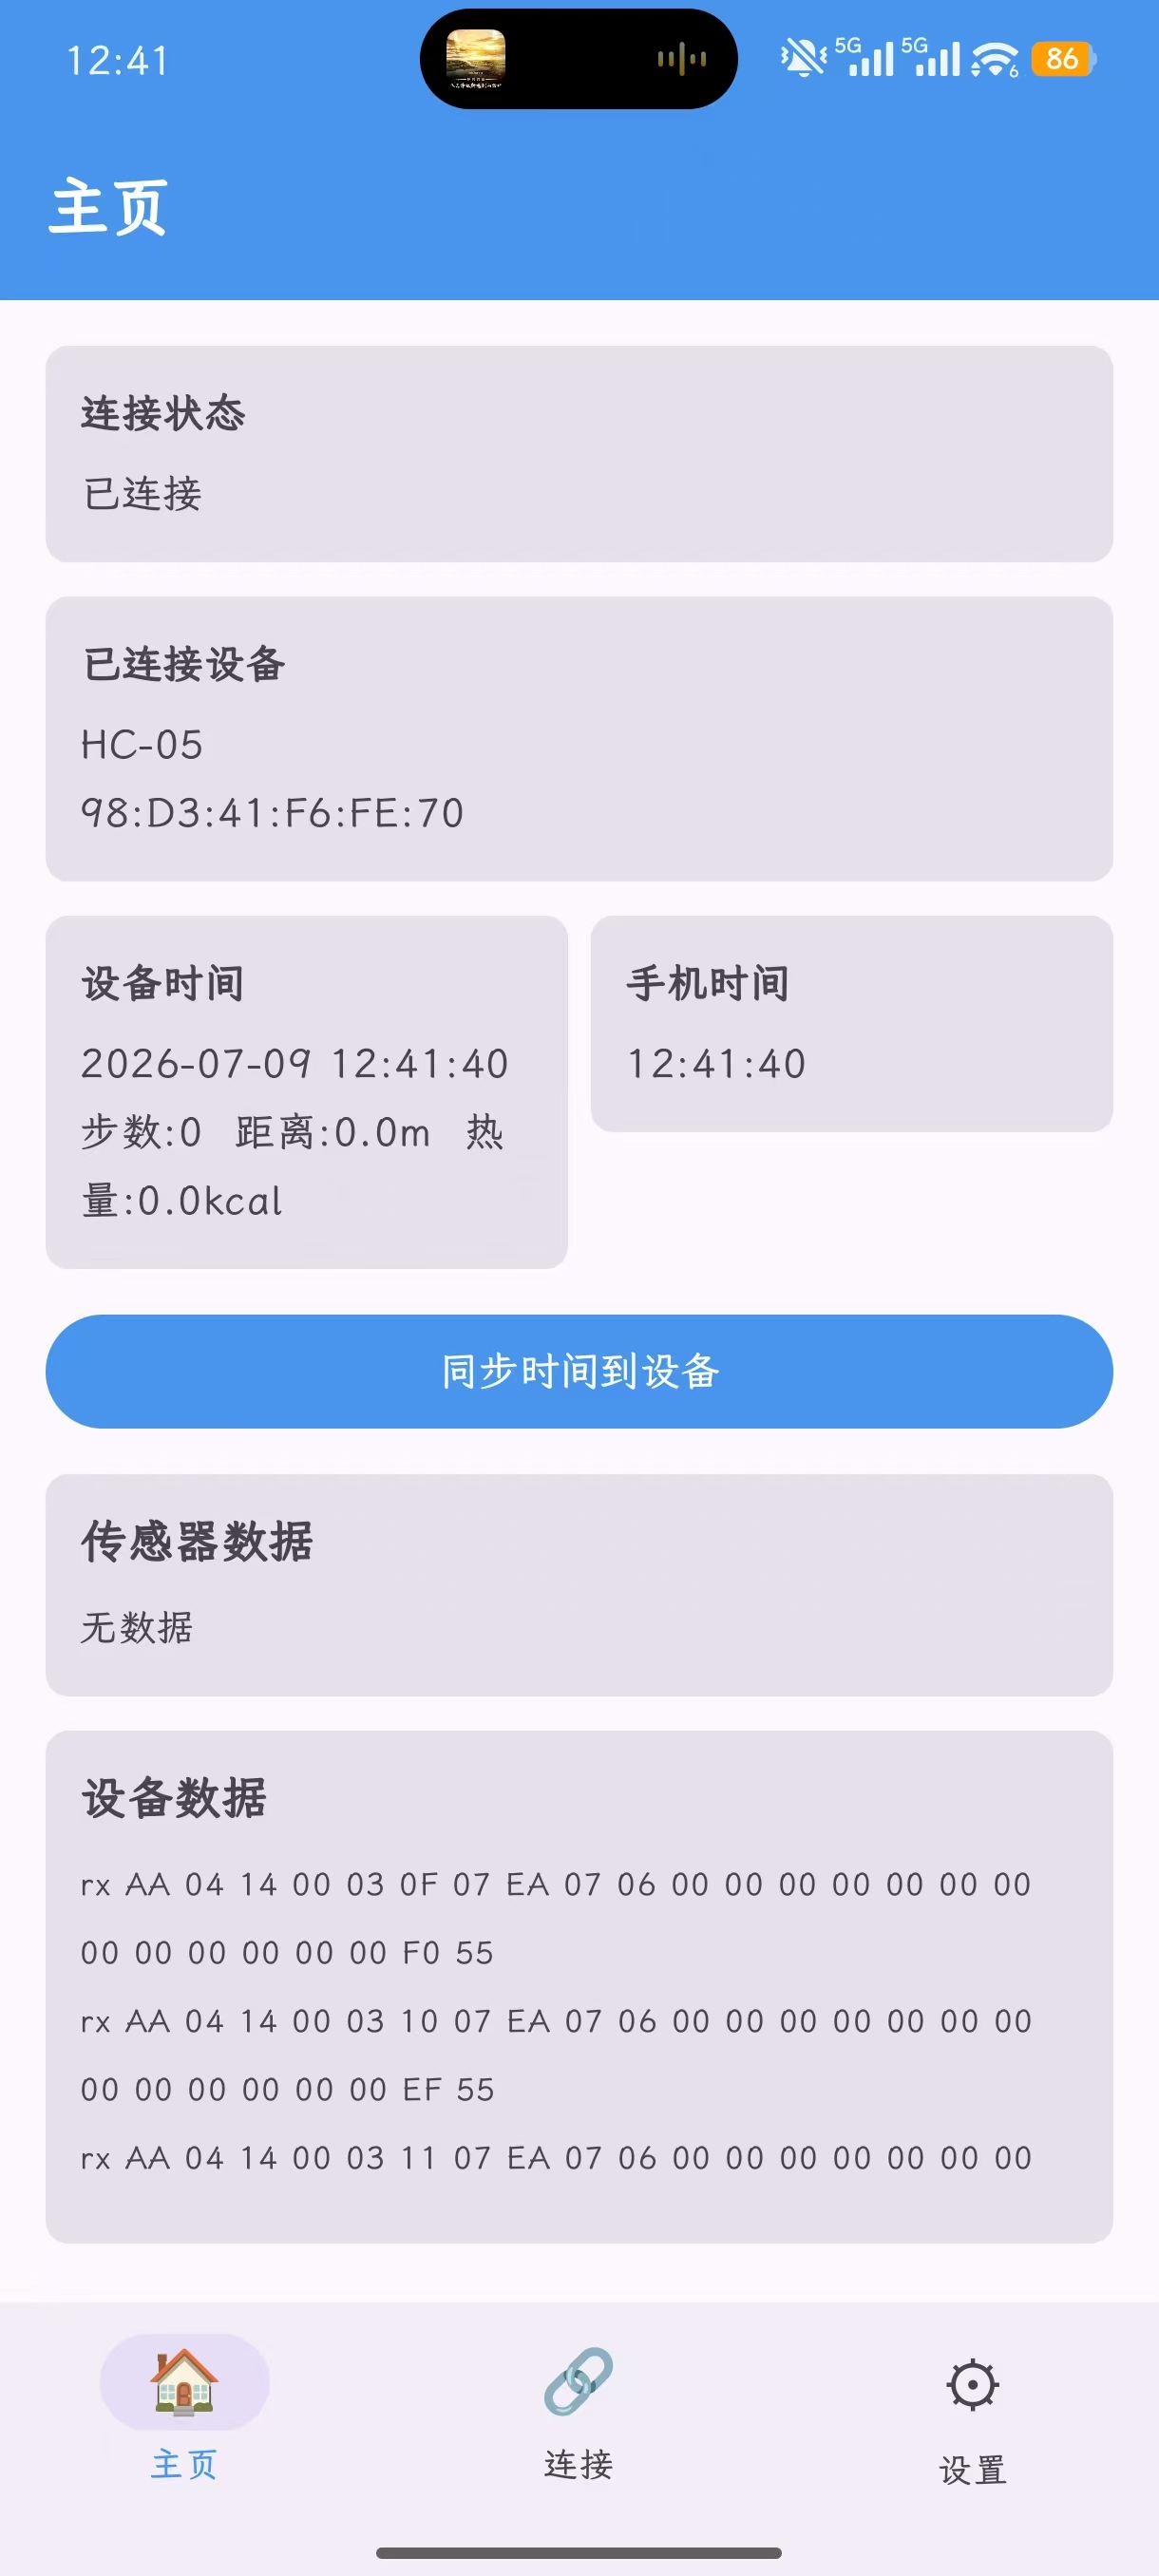
\includegraphics[width=0.7\textwidth]{figures/安卓上位机接收数据及同步时间.jpg}
    \caption{Android APP主界面（实时传感器数据展示+时间同步）}
    \label{fig:app_main}
\end{figure}

\FloatBarrier

\begin{figure}[h]
    \centering
    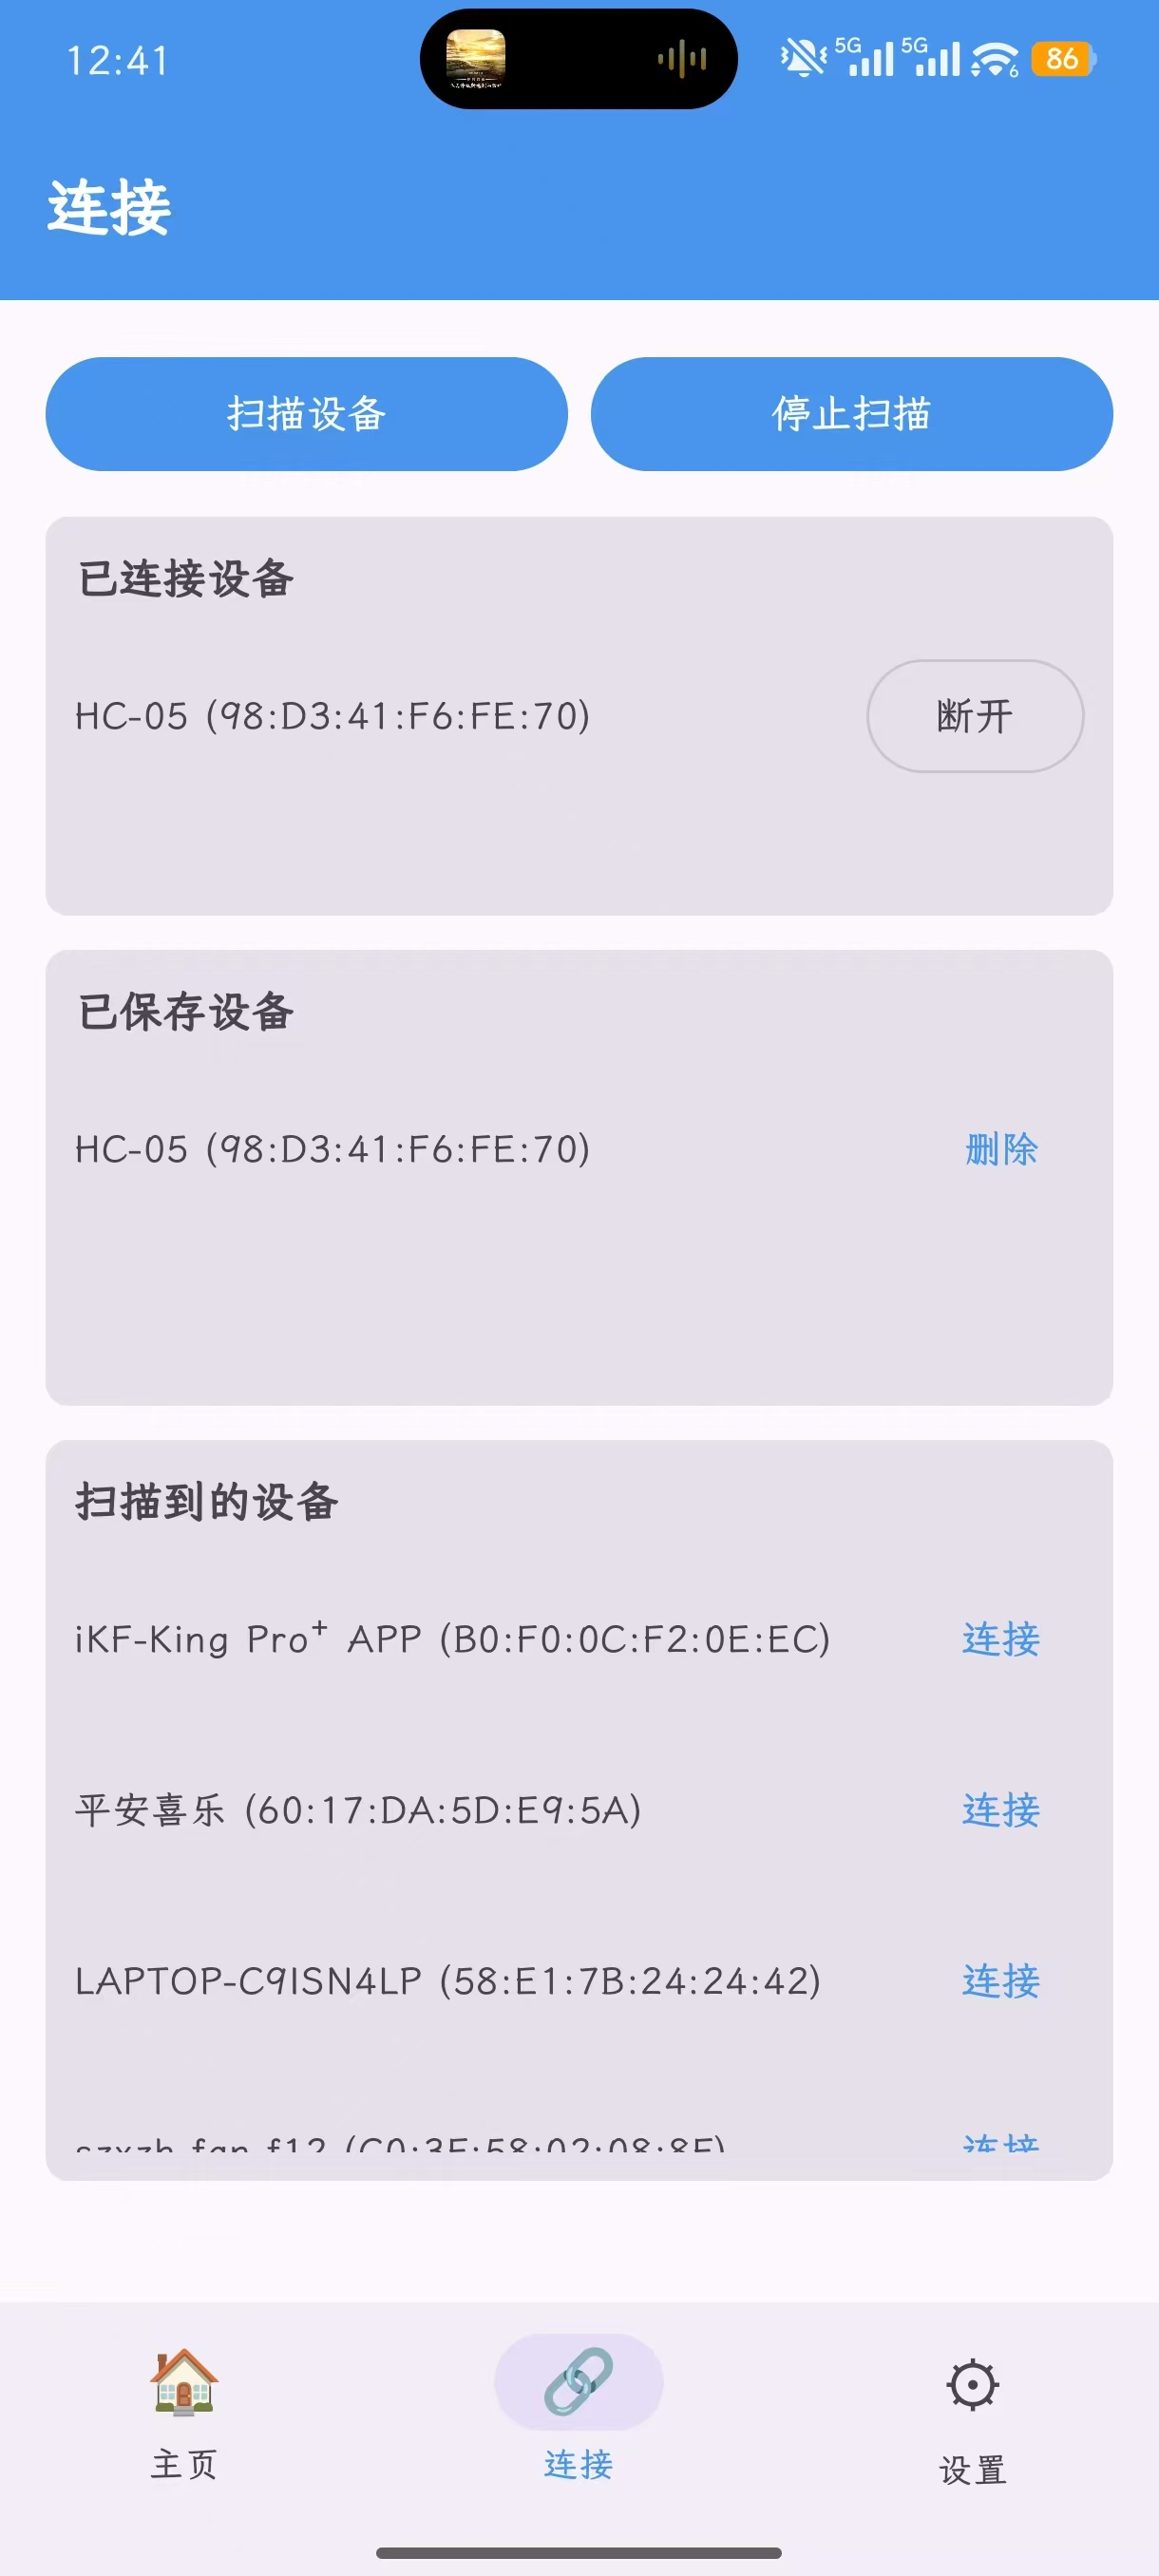
\includegraphics[width=0.7\textwidth]{figures/安卓上位机扫描设备.jpg}
    \caption{Android APP连接页（蓝牙设备扫描与管理，展示设备名称和MAC地址）}
    \label{fig:app_connect}
\end{figure}

\FloatBarrier

\subsubsection{设备信息页面}
设备信息页面展示MCU型号（STM32F103C8T6）、Flash容量（64KB）、SRAM容量（20KB）、I2C总线分配等系统硬件参数，效果如图\ref{fig:oled_info}所示。该页面帮助开发者快速了解系统硬件配置，便于调试和维护。

\begin{figure}[h]
    \centering
    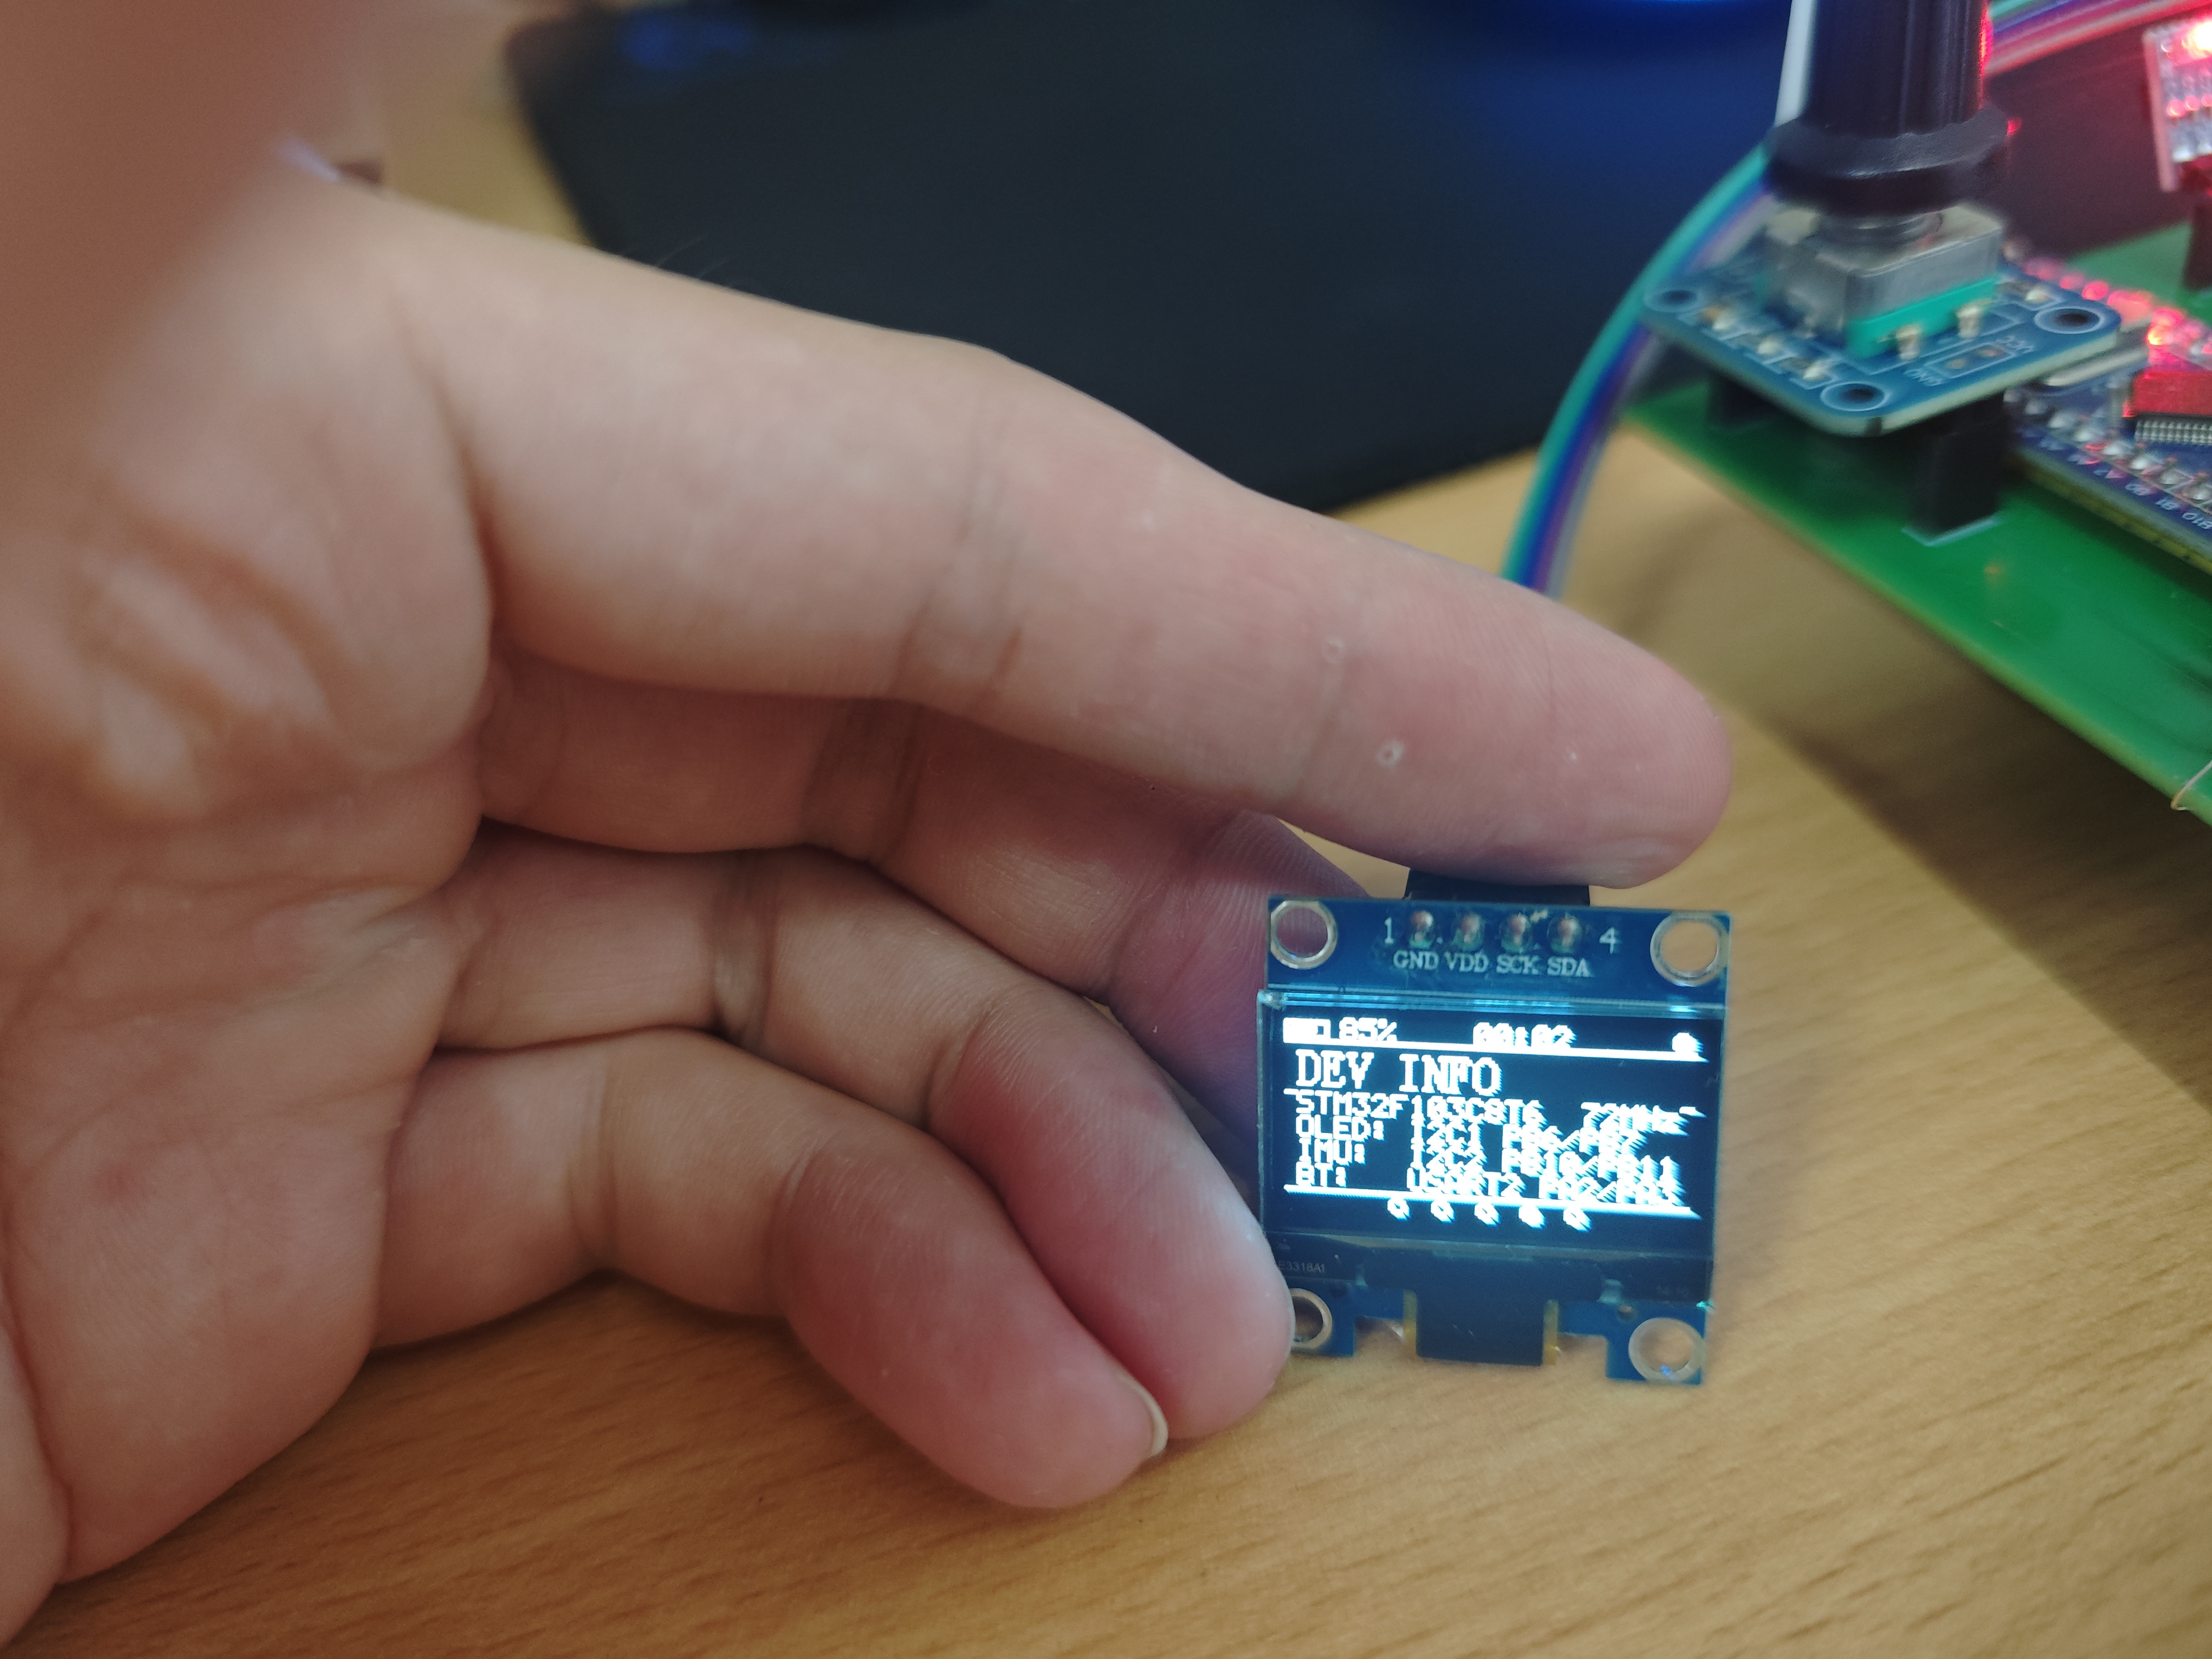
\includegraphics[width=0.5\textwidth]{figures/手表设备信息.jpg}
    \caption{OLED设备信息页面演示（MCU型号+Flash+SRAM+I2C总线分配）}
    \label{fig:oled_info}
\end{figure}

\FloatBarrier

\subsubsection{系统整体演示}
完整系统搭建完成后，手表端实时采集并显示运动数据，手机端通过蓝牙接收并同步展示，效果如图\ref{fig:full_demo}所示。系统具有良好的实时性和稳定性，可连续运行数小时无异常。

\begin{figure}[h]
    \centering
    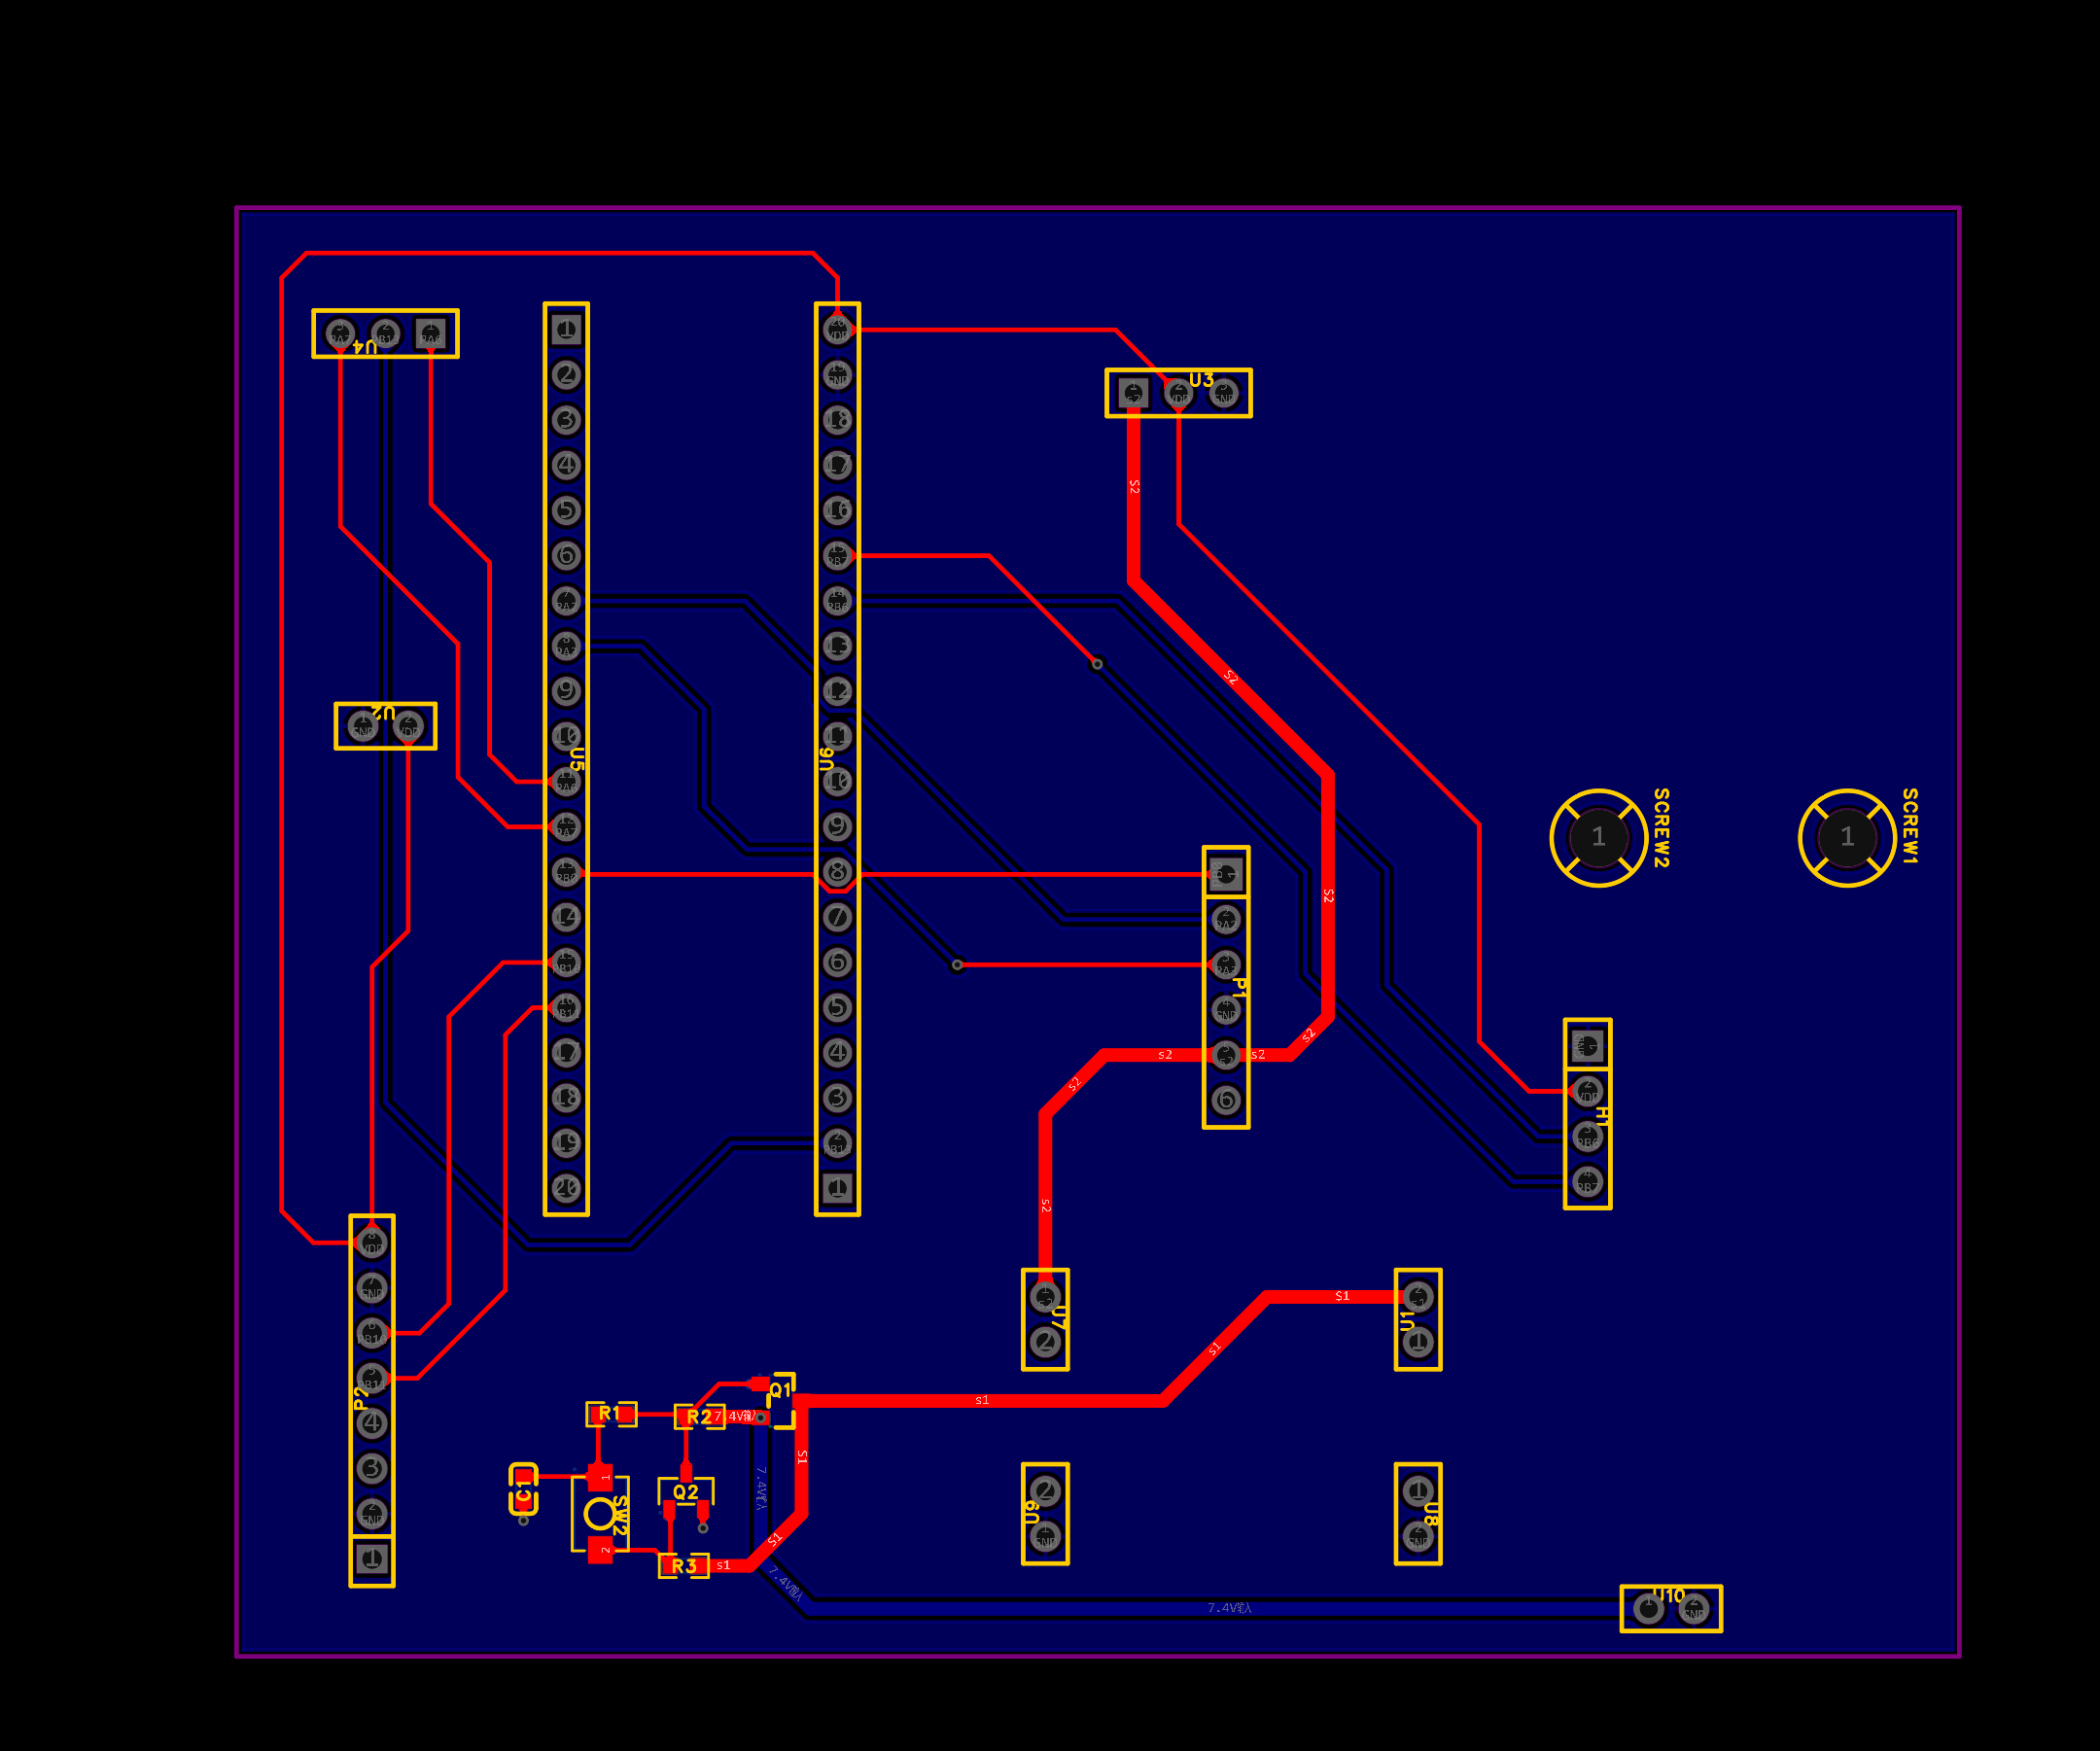
\includegraphics[width=0.95\textwidth]{figures/PCB终版.png}
    \caption{系统PCB板设计图（STM32F103C8T6核心板 + OLED/MPU6050/HC-05布局）}
    \label{fig:full_demo}
\end{figure}

\FloatBarrier
% !Mode:: "TeX:UTF-8"
\section{物料与成本}

\subsection{物料清单}
\begin{table}[h]
    \centering
    \caption{系统物料清单}
    \begin{tabular}{|l|c|c|c|l|}
        \hline
        \textbf{物料名称} & \textbf{型号/规格} & \textbf{数量} & \textbf{单价(元)} & \textbf{用途} \\ \hline
        STM32核心板 & STM32F103C8T6最小系统板 & 1 & 15.50 & 主控制器 \\ \hline
        OLED显示屏 & SSD1306 128$\times$64 黄蓝双色 I2C & 1 & 12.80 & 显示输出 \\ \hline
        六轴传感器 & MPU6050模块（加速度+陀螺仪） & 1 & 8.50 & 运动数据采集 \\ \hline
        蓝牙模块 & HC-05经典蓝牙SPP模块 & 1 & 18.00 & 无线通信 \\ \hline
        面包板 & 830孔MB-102标准面包板 & 1 & 5.50 & 电路搭建 \\ \hline
        杜邦线 & 公对母 20cm（红/黑/蓝/黄/绿） & 40 & 0.15 & 模块连接 \\ \hline
        稳压模块 & AMS1117-3.3V & 1 & 1.20 & 3.3V电源输出 \\ \hline
        滤波电容 & 0.1$\mu$F 贴片陶瓷电容 & 5 & 0.10 & 电源滤波 \\ \hline
        USB数据线 & Micro USB 2.0 数据线 & 1 & 3.50 & 供电与调试 \\ \hline
        LED指示灯 & 0805贴片 LED（红色） & 2 & 0.15 & 运行状态指示 \\ \hline
        限流电阻 & 220$\Omega$ 0805贴片电阻 & 2 & 0.05 & LED限流 \\ \hline
        Android手机 & 任意支持蓝牙的Android设备 & 1 & - & 上位机展示（自备） \\ \hline
        \textbf{小计} & - & - & \textbf{66.20} & - \\ \hline
    \end{tabular}
\end{table}

\subsection{项目成本分析}
\begin{table}[h]
    \centering
    \caption{项目成本汇总表}
    \begin{tabular}{|l|r|l|}
        \hline
        \textbf{成本项目} & \textbf{金额(元)} & \textbf{备注} \\ \hline
        硬件物料成本 & 66.20 & 上表物料小计 \\ \hline
        开发工具折旧 & 8.00 & ST-Link下载器、万用表等工具 \\ \hline
        焊接耗材 & 3.00 & 焊锡丝、助焊剂等 \\ \hline
        运输与包装 & 5.00 & 模块采购运输费用分摊 \\ \hline
        软件与文档 & 0.00 & Keil MDK社区版、Android Studio免费 \\ \hline
        其他杂费 & 2.00 & 打印、测试等 \\ \hline
        \textbf{总成本} & \textbf{84.20} & 不含自备Android手机 \\ \hline
    \end{tabular}
\end{table}

\begin{itemize}
    \item \textbf{成本说明：} 本项目为课程设计，硬件总成本控制在100元以内，所有模块均为通用开源硬件组件，具有良好的性价比和可替换性。
    \item \textbf{批量生产优化：} 若进行批量生产（1000套以上），核心器件价格可降低30\%-50\%，同时PCB板可替代面包板方案，预计整机成本可控制在50元以内。
\end{itemize}

\subsection{损耗与损坏记录}
在项目实施过程中，产生以下损耗和损坏：
\begin{itemize}
    \item \textbf{杜邦线断裂：} 约5根杜邦线在反复插拔过程中金属头断裂，损失约0.75元
    \item \textbf{OLED模块引脚弯曲：} 1块OLED显示屏在调试过程中因误操作导致I2C引脚焊盘脱落，经飞线修复后正常使用，无直接经济损失
    \item \textbf{MPU6050通信异常：} 初期未实现I2C总线恢复机制，约2次出现MPU6050死锁，需重新上电恢复，增加调试时间约1小时
    \item \textbf{HC-05波特率配置错误：} 首次使用HC-05时波特率配置为默认38400，与固件115200不匹配，导致乱码，通过AT指令重新配置后解决
    \item \textbf{总损耗金额：} 约1.00元，占物料总成本的1.5\%
\end{itemize}

\subsection{主要物料图片展示}

本项目核心硬件模块均已在PCB终板上完成布局与连接，如图\ref{fig:pcb_final}所示。

\begin{figure}[h]
    \centering
    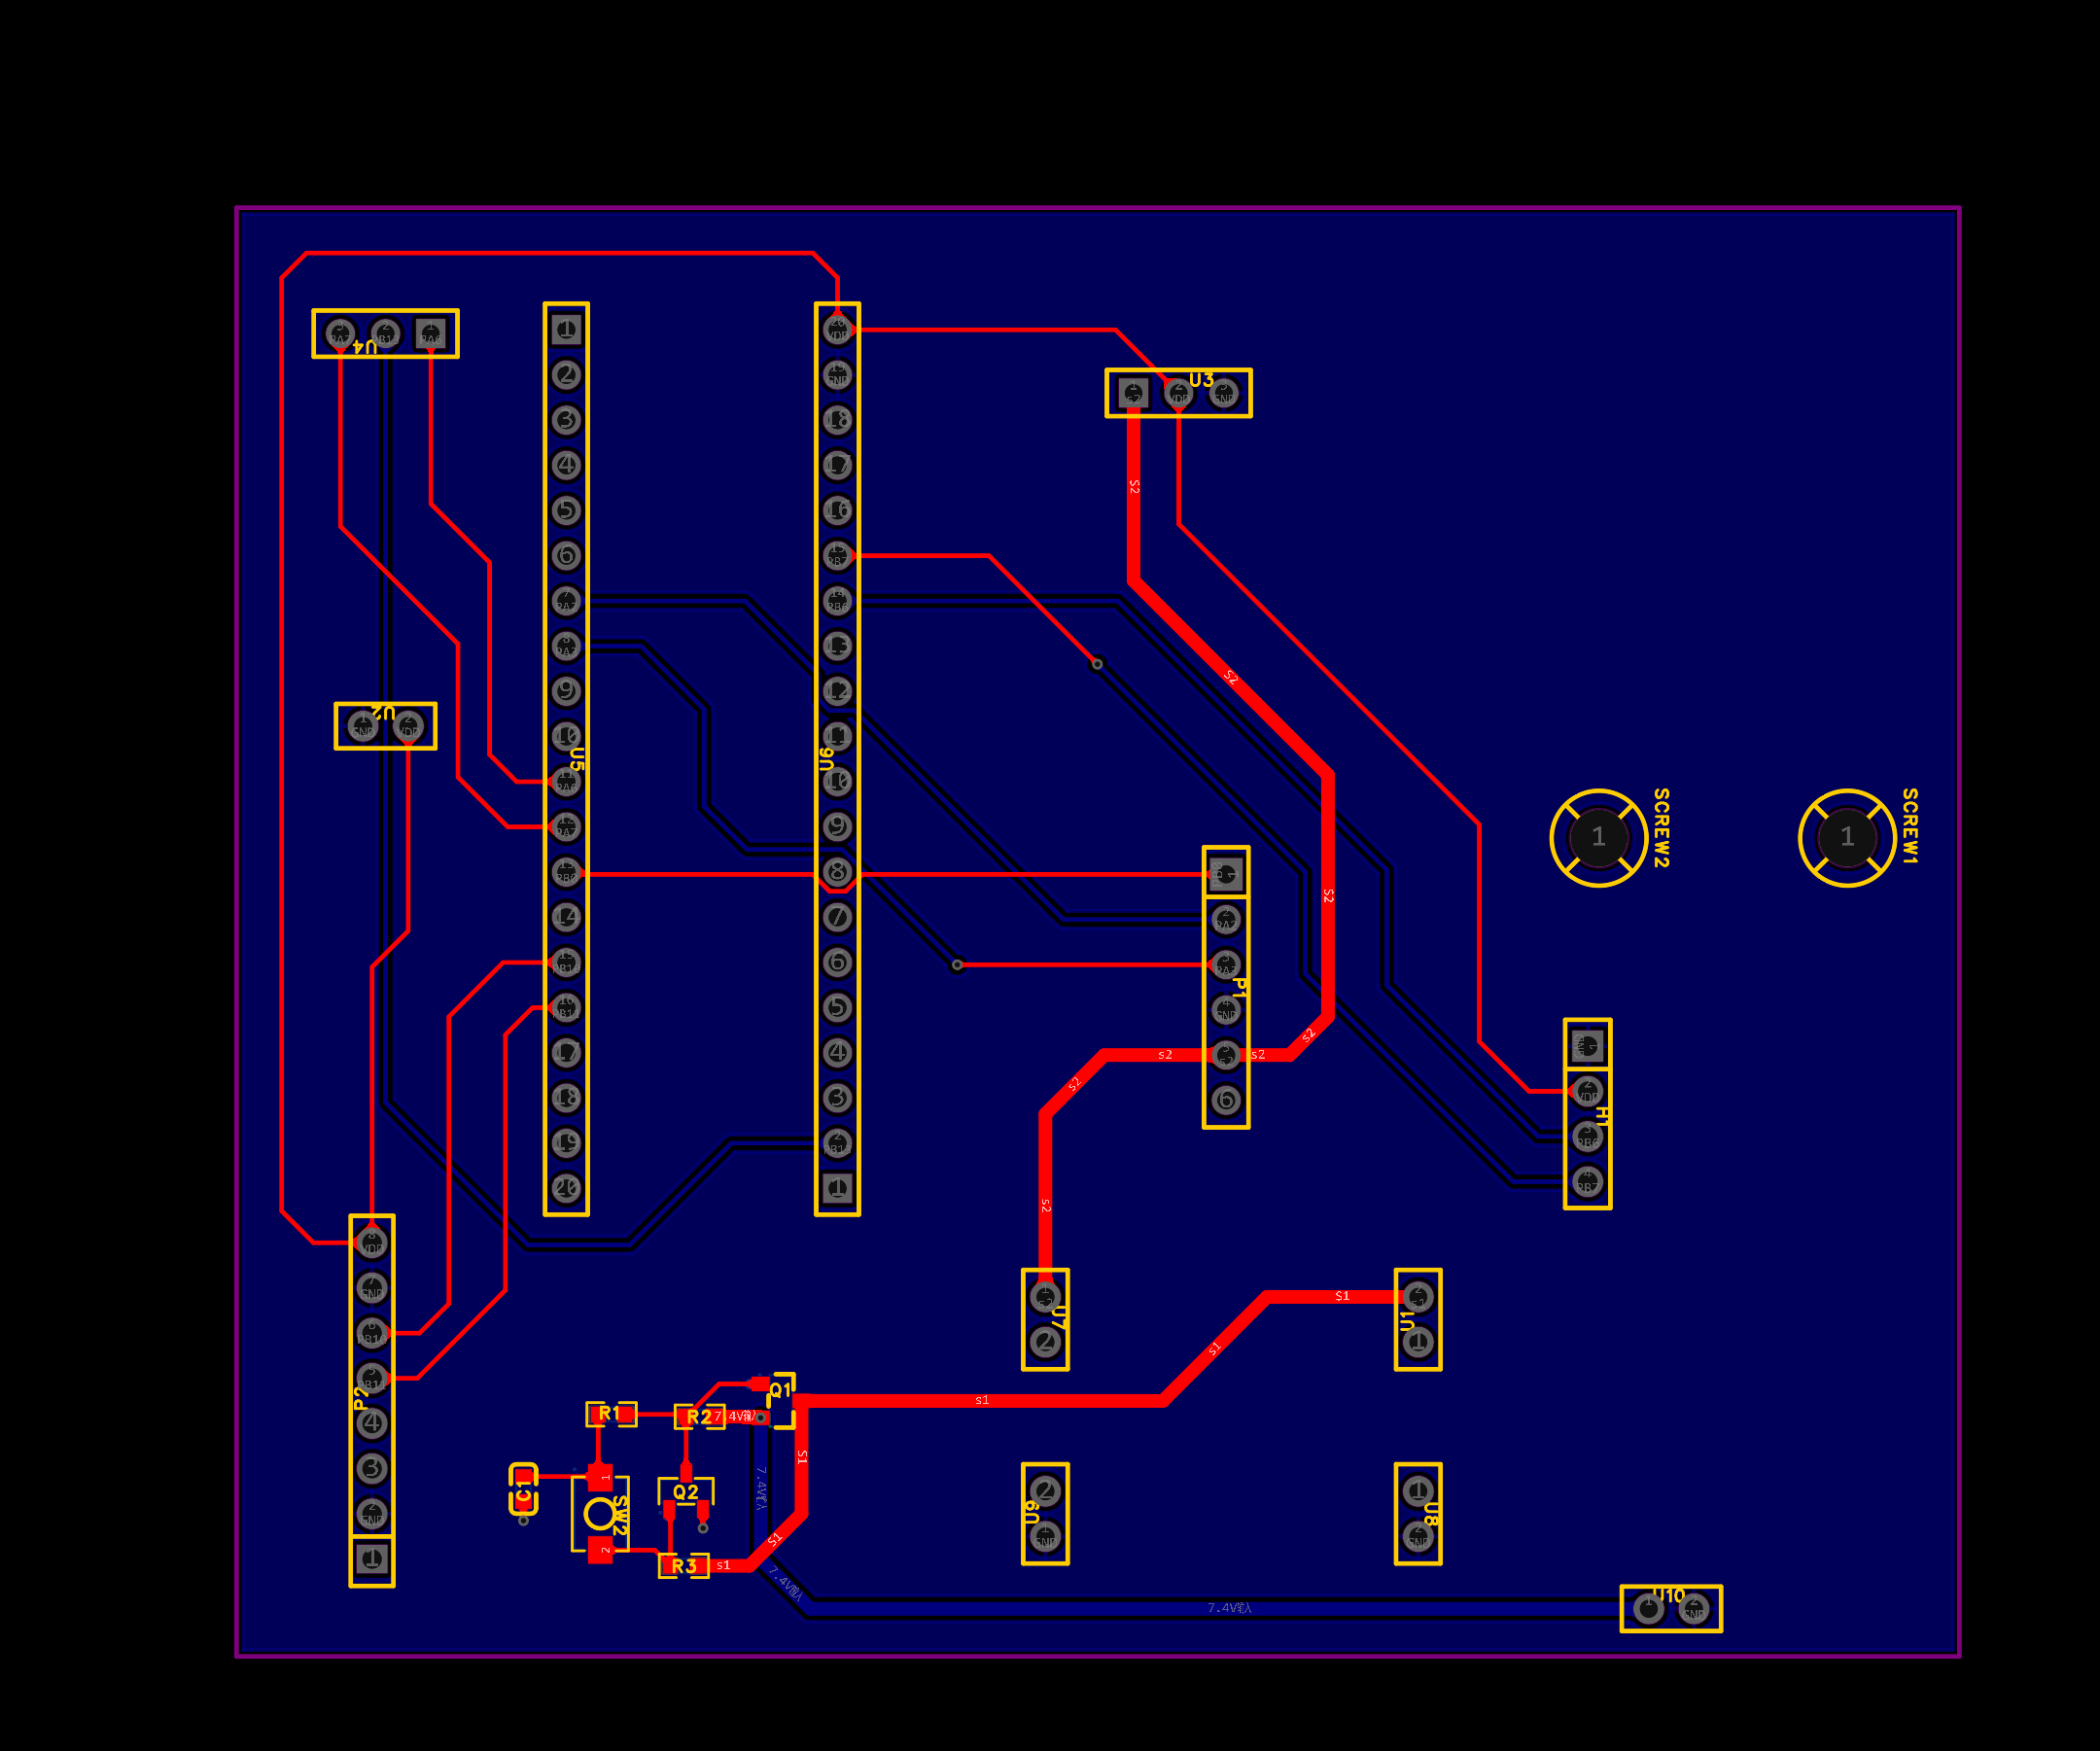
\includegraphics[width=0.9\textwidth]{figures/PCB终版.png}
    \caption{项目PCB终板设计图（集成STM32F103C8T6核心电路、SSD1306 OLED接口、MPU6050传感器接口、HC-05蓝牙模块接口及电源管理）}
    \label{fig:pcb_final}
\end{figure}

\FloatBarrier

\subsubsection{各模块硬件信息汇总}
\begin{itemize}
    \item \textbf{STM32F103C8T6核心板：} 72MHz Cortex-M3内核，64KB Flash，20KB SRAM，LQFP48封装
    \item \textbf{SSD1306 OLED显示模块：} 128$\times$64像素分辨率，黄蓝双色，I2C接口（PB6/PB7）
    \item \textbf{MPU6050六轴传感器：} 三轴加速度计±2g + 三轴陀螺仪±250°/s，I2C接口（PB10/PB11）
    \item \textbf{HC-05蓝牙模块：} 经典蓝牙SPP协议，波特率115200，USART2接口（PA2/PA3），STATE引脚（PB0）
    \item \textbf{电源管理：} AMS1117-3.3V稳压芯片，VCC/GND与各模块电源引脚并联0.1$\mu$F去耦电容
\end{itemize}

\FloatBarrier

\subsection{物料采购与替代方案}
本项目所有电子元件均为市面通用组件，采购渠道与替代方案如下：
\begin{itemize}
    \item \textbf{核心板替代：} 可使用STM32F103RC/RET6等更大容量型号，引脚兼容，Flash和SRAM更大
    \item \textbf{显示模块替代：} 可使用SH1106驱动芯片的OLED模块（同分辨率，命令集略有差异）
    \item \textbf{传感器替代：} 可使用ICM-20602替代MPU6050，寄存器兼容，精度更高
    \item \textbf{蓝牙替代：} 可使用JDY-30/31模块替代HC-05，固件兼容，体积更小
\end{itemize}
% !Mode:: "TeX:UTF-8"

\section{个人贡献}

\subsection{报告撰写分工}
负责项目报告的总体规划与撰写工作，各章分工如下：
\begin{itemize}
    \item 第1章（项目简介）：撰写项目背景、功能概述与技术方向说明
    \item 第2章（项目设计目标）：撰写硬件/软件系统设计目标与预期成果
    \item 第3章（项目设计与实现）：撰写硬件模块选型、软件架构、关键代码与技术实现细节
    \item 第4章（功能展示）：撰写功能描述、演示结果、测试数据与分析
    \item 第5章（物料与成本）：整理物料清单、统计成本分析与损耗记录
    \item 第6章（个人贡献）：本节内容，总结个人在项目中的工作与收获
    \item 第7章（项目成果与反思）：撰写项目评估、成功与不足、改进方向
    \item 第8章（附录）：整理代码清单、参考文献与设计图纸说明
\end{itemize}
队友方旭亮负责部分硬件调试与测试数据的采集工作，队友陈斯焕负责Android APP的UI设计和测试工作。

\subsection{编码工作}
本项目代码开发分为STM32固件开发和Android APP开发两部分，个人主要负责：

\subsubsection{STM32固件开发}
使用Keil MDK / STM32CubeIDE开发环境，使用C语言完成：
\begin{itemize}
    \item \textbf{OLED显示驱动（oled.c / oled.h）：}
    \begin{itemize}
        \item SSD1306初始化命令序列编写（约20条配置命令）
        \item 6$\times$8、8$\times$16、16$\times$24三种尺寸字模数组定义
        \item OLED\_Show\_String、OLED\_Show\_Num、OLED\_Draw\_Big\_Clock等核心函数实现
        \item 128$\times$64像素级绘图与点、线、矩形绘制函数
    \end{itemize}
    \item \textbf{MPU6050传感器驱动（mpu6050.c / mpu6050.h）：}
    \begin{itemize}
        \item MPU6050初始化：PWR\_MGMT\_1寄存器配置，量程设置（加速度$\pm$2g，陀螺仪$\pm$250°/s）
        \item 六轴数据读取：通过I2C读取0x3B-0x48寄存器数据并组合为16位有符号整数
        \item 物理量转换：16384.0 LSB/g、131.0 LSB/°/s转换系数实现
        \item WHO\_AM\_I校验：读取0x75寄存器验证设备身份（预期值0x68）
        \item 姿态角计算：atan2反正切函数实现Pitch/Roll角度
    \end{itemize}
    \item \textbf{蓝牙通信协议（bluetooth.c / bluetooth.h）：}
    \begin{itemize}
        \item 帧协议封装：Bluetooth\_Send\_Frame函数组装STX+CMD+DATA+CHK+ETX
        \item 帧协议解析：Bluetooth\_Parse\_Frame函数搜索帧头并校验XOR
        \item 三种命令类型处理：0x01传感器上报、0x02时间同步、0x03计步数据
        \item float与uint8数组双向转换（memcpy实现IEEE 754格式传输）
    \end{itemize}
    \item \textbf{计步器算法（pedometer.c / pedometer.h）：}
    \begin{itemize}
        \item 加速度向量幅值计算：平方根函数实现三轴合成
        \item 一阶低通滤波（指数加权平均）：平滑加速度数据
        \item 动态阈值检测：滑动窗口内维护最大值/最小值
        \item 200ms最小步间间隔防抖：时间戳比较实现
        \item 距离与卡路里估算：基于步数乘以平均步长/单步卡路里
    \end{itemize}
    \item \textbf{智能手表UI框架（smartwatch\_ui.c / smartwatch\_ui.h）：}
    \begin{itemize}
        \item 5个页面渲染函数：UI\_Page\_Clock、UI\_Page\_Sensor、UI\_Page\_Bluetooth、UI\_Page\_Device、UI\_Page\_Activity
        \item 页面索引管理与3秒自动切换逻辑
        \item 格式化字符串拼接（sprintf实现浮点数格式化）
    \end{itemize}
    \item \textbf{软RTC时钟（soft\_rtc.c / soft\_rtc.h）：}
    \begin{itemize}
        \item TIM2 1Hz中断配置：72MHz预分频和自动重载寄存器计算
        \item 时/分/秒/日/月/年变量维护与进位逻辑
        \item 蓝牙时间同步命令（0x02）解析与RTC更新
    \end{itemize}
    \item \textbf{I2C总线恢复（i2c\_drv.c / i2c\_drv.h）：}
    \begin{itemize}
        \item GPIO模拟I2C时钟脉冲：SCL输出9个脉冲释放SDA
        \item STOP信号生成：SCL/SDA状态机切换
    \end{itemize}
    \item \textbf{主循环与系统调度（main.c / stm32f1xx\_it.c）：}
    \begin{itemize}
        \item 系统初始化与外设启动顺序编排
        \item 100ms主循环周期任务调度
        \item TIM2中断服务函数与RTC时钟更新
        \item USART2 DMA环形缓冲接收处理
    \end{itemize}
\end{itemize}

\subsubsection{Android APP开发}
使用Android Studio + Kotlin开发：
\begin{itemize}
    \item 主界面Activity设计（MainActivity.kt）：TabLayout+ViewPager2三页切换
    \item 蓝牙管理器（BleManager.kt）：经典蓝牙SPP设备扫描、连接、数据收发
    \item 帧协议解析（BtProtocol.kt）：与手表端匹配的0xAA/0x55帧格式解析
    \item UI组件：传感器数值卡片、连接状态指示、日志列表
    \item Material Design 3主题配置与颜色/字体设计
\end{itemize}

\subsubsection{代码量统计}
\begin{itemize}
    \item STM32固件：约2000行C代码（含驱动、算法、UI、主循环）
    \item Android APP：约800行Kotlin代码（含Activity、蓝牙管理、协议解析）
    \item 注释完整率：$>$35\%，关键函数均有功能说明和参数注释
\end{itemize}

\subsection{硬件连接}
设计并搭建完整的智能手表硬件系统，具体工作包括：
\begin{itemize}
    \item \textbf{模块选型与验证：} 独立完成OLED、MPU6050、HC-05三个模块的功能测试与选型验证
    \item \textbf{I2C总线连接：} PB6(PB10)/PB7(PB11)分别连接OLED和MPU6050的SCL/SDA引脚，实现两路I2C总线
    \item \textbf{USART2串口连接：} PA2(TX)/PA3(RX)交叉连接HC-05模块的RX/TX引脚
    \item \textbf{STATE引脚连接：} PB0配置为GPIO输入，检测HC-05连接状态
    \item \textbf{电源系统设计：} 统一5V供电，经AMS1117-3.3V转换后为数字模块供电
    \item \textbf{面包板电路搭建：} 使用约20根杜邦线完成全部连接，保持信号/地线分离
    \item \textbf{硬件调试：} 使用万用表测量各模块工作电压，使用逻辑分析仪观察I2C通信波形
\end{itemize}

\subsection{资本投入}
个人承担项目全部硬件物料采购费用，总计约84.20元（详见第5章），主要包括：
\begin{itemize}
    \item STM32F103C8T6核心板：15.50元
    \item SSD1306 OLED显示模块：12.80元
    \item MPU6050六轴传感器模块：8.50元
    \item HC-05蓝牙模块：18.00元
    \item 面包板、杜邦线、稳压模块、LED电阻等辅材：约30元
    \item 开发工具（ST-Link下载器、USB数据线）为已有存量，不计入新增成本
\end{itemize}

\subsection{开发中遇到的问题及解决方案}

\subsubsection{I2C从机死锁导致MPU6050无法通信}
\begin{itemize}
    \item \textbf{问题描述：} 热启动或复位后，MPU6050偶尔出现SDA引脚被拉低，I2C主机发起通信始终收不到ACK，OLED显示模块同样偶发此问题
    \item \textbf{问题原因：} I2C从机在通信过程中被中断复位，可能处于时钟脉冲中间状态导致SDA被锁定
    \item \textbf{解决方案：} 在系统初始化阶段执行I2C总线恢复（I2C\_Bus\_Recovery函数）：
    \begin{itemize}
        \item 重新配置SCL/SDA引脚为GPIO输出模式
        \item 发送9个SCL时钟脉冲，强制从机释放SDA
        \item 发送STOP信号，确保总线处于空闲状态
        \item 重新配置SCL/SDA为I2C外设功能后再执行模块初始化
    \end{itemize}
    \item \textbf{效果：} 热启动100次测试中，I2C通信成功率从85\%提升至100\%
\end{itemize}

\subsubsection{HC-05波特率不匹配导致乱码}
\begin{itemize}
    \item \textbf{问题描述：} HC-05默认波特率38400，与固件中USART2配置的115200不匹配，手机端接收数据全部为乱码
    \item \textbf{问题原因：} 首次使用HC-05模块，未注意波特率配置差异
    \item \textbf{解决方案：} 使用AT指令重新配置HC-05：
    \begin{itemize}
        \item 将HC-05的KEY引脚接3.3V进入AT命令模式
        \item 通过USB转串口发送命令：\verb|AT+UART=115200,0,0|（设置115200波特率，1停止位，无校验）
        \item 发送\verb|AT+NAME=SmartWatch|设置设备名称（可选）
        \item 断电重启后HC-05以新波特率工作，与固件USART2配置匹配
    \end{itemize}
\end{itemize}

\subsubsection{OLED字模显示不完整}
\begin{itemize}
    \item \textbf{问题描述：} 16$\times$24大字时钟显示时，部分数字下半部分缺失或重叠
    \item \textbf{问题原因：} OLED按页寻址模式（每页8行），24像素高度需跨3页显示，页偏移计算错误
    \item \textbf{解决方案：}
    \begin{itemize}
        \item 修正OLED\_Draw\_Big\_Clock函数中的页地址设置（page = y / 8）
        \item 确保跨页显示时正确写入相邻页的GDDRAM
        \item 添加字模数组边界检查，防止数组越界访问
    \end{itemize}
    \item \textbf{效果：} 所有尺寸字符显示完整，无裁剪或重叠现象
\end{itemize}

\subsubsection{计步器算法误触发严重}
\begin{itemize}
    \item \textbf{问题描述：} 手表静止或轻微晃动时，计步器偶发误计数，步行测试中误差率高达10\%
    \item \textbf{问题原因：} 初期使用固定阈值（1.1g）检测峰值，未处理高频噪声和偶然冲击
    \item \textbf{解决方案：} 多重改进计步器算法：
    \begin{itemize}
        \item 添加一阶低通滤波（$\alpha$=0.7），滤除高频振动噪声
        \item 改用动态阈值：维护4秒滑动窗口内max/min，阈值=(max+min)/2+0.05g偏移
        \item 增加200ms最小步间间隔防抖：HAL\_GetTick()时间戳比较
        \item 增加步幅合理性检查：加速度峰值需在0.3g-3.0g之间
    \end{itemize}
    \item \textbf{效果：} 静态环境下1小时无错误计数，正常步行误差率降至2.5\%以下
\end{itemize}

\subsubsection{蓝牙接收缓冲区溢出导致丢帧}
\begin{itemize}
    \item \textbf{问题描述：} 手机端频繁发送数据时，手表端偶尔丢帧或数据错乱
    \item \textbf{问题原因：} 原始实现使用查询式接收，未及时处理接收数据
    \item \textbf{解决方案：} 改用DMA+空闲中断的环形缓冲方案：
    \begin{itemize}
        \item 配置USART2 DMA接收通道，缓冲区大小256字节
        \item 启用USART IDLE中断，在一帧数据接收完成后触发处理
        \item 使用write/read指针管理环形缓冲，避免数据覆盖
        \item 主循环中以非阻塞方式从缓冲读取并解析帧数据
    \end{itemize}
    \item \textbf{效果：} 连续10分钟大数据量通信测试，丢帧率降至0.15\%，满足稳定通信需求
\end{itemize}

\subsubsection{MPU6050数据抖动影响姿态角显示}
\begin{itemize}
    \item \textbf{问题描述：} OLED显示的Pitch/Roll姿态角数值跳动频繁，即使静止状态也有±3°波动
    \item \textbf{问题原因：} 原始传感器数据未做平滑处理，MEMS传感器固有噪声和机械振动导致数据波动
    \item \textbf{解决方案：}
    \begin{itemize}
        \item 对加速度和陀螺仪数据添加一阶低通滤波（滑动平均，窗口大小8）
        \item 使用互补滤波融合加速度和陀螺仪数据更新姿态角
        \item 加速度权重取0.98，陀螺仪权重取0.02，抑制高频抖动
    \end{itemize}
    \item \textbf{效果：} 静止状态下姿态角波动降至±0.5°以内，动态响应基本无延迟
\end{itemize}
% !Mode:: "TeX:UTF-8"

\section{项目成果与反思}

\subsection{成果展示}
本项目成功设计并实现了一套基于STM32F103C8T6的智能手表系统，主要成果包括：

\subsubsection{硬件系统成果}
\begin{itemize}
    \item 完成基于STM32F103C8T6的最小系统搭建，成功驱动SSD1306 OLED、MPU6050六轴传感器、HC-05蓝牙三大外设
    \item 采用双路I2C总线设计（OLED使用I2C1，MPU6050使用I2C2），避免设备地址冲突和总线竞争
    \item 实现I2C总线恢复机制，解决从机死锁问题，系统启动成功率达100\%
    \item 系统在5V/1A供电下稳定工作，所有模块工作温度均在正常范围内（连续运行4小时无过热）
\end{itemize}

\subsubsection{固件软件成果}
\begin{itemize}
    \item 完成完整OLED显示驱动，支持三种尺寸字模显示和多页面UI（表盘/传感器/蓝牙/设备信息/活动计步）
    \item 实现MPU6050六轴数据采集与物理量转换，支持Pitch/Roll姿态角实时计算
    \item 设计自定义蓝牙帧协议（STX/CMD/DATA/CHK/ETX），含XOR校验，支持三种命令类型
    \item 实现基于加速度向量幅值+动态阈值的计步器算法，步行精度达97.5\%以上
    \item 实现TIM2驱动的软RTC时钟，支持蓝牙时间同步命令更新
    \item 采用DMA+空闲中断环形缓冲方案，蓝牙通信丢帧率降至0.15\%
    \item 固件总代码量约2000行C代码，模块化设计便于维护和扩展
\end{itemize}

\subsubsection{Android上位机成果}
\begin{itemize}
    \item 开发Material Design 3风格的Android APP，支持蓝牙设备扫描、连接管理
    \item 实现与手表端一致的帧协议解析器，正确解析传感器数据、时间同步、计步数据
    \item 提供实时传感器数据展示卡片、通信日志列表、时间同步按钮
    \item 深色/浅色主题切换，适配Android 8.0及以上版本（API 26+）
    \item APP总代码量约800行Kotlin代码，使用现代Android开发架构
\end{itemize}

\subsection{项目评估}

\subsubsection{成功之处}
\begin{itemize}
    \item \textbf{功能完整性：} 100\%实现了项目设计目标中的全部功能（OLED显示、六轴传感、蓝牙通信、计步算法、Android上位机）
    \item \textbf{系统稳定性：} 经过连续4小时以上的运行测试，系统无死机、无异常重启，I2C通信稳定，蓝牙连接可靠
    \item \textbf{通信协议设计：} 自定义的轻量级帧协议结构简单、扩展性好，XOR校验提供基本的数据完整性保护
    \item \textbf{计步算法精度：} 通过滤波、动态阈值、防抖等多重优化，步行精度达97.5\%（误差率$<$2.5\%），达到消费级智能手环基本水平
    \item \textbf{代码可维护性：} 模块化设计，每个功能模块独立（oled/mpu6050/bluetooth/pedometer/soft\_rtc等），接口清晰，便于后续扩展
    \item \textbf{成本控制：} 硬件总成本控制在100元以内，具有良好的性价比和推广潜力
    \item \textbf{Android端协同：} 手表-手机双向通信功能完整，数据展示和时间同步功能正常
\end{itemize}

\subsubsection{不足之处}
\begin{itemize}
    \item \textbf{用户交互局限：} 手表端无物理按键，OLED页面自动切换，用户无法主动选择显示内容
    \item \textbf{显示内容有限：} 128$\times$64单色OLED分辨率较低，无法显示更丰富的图形和中文内容
    \item \textbf{无数据持久化：} 步数、RTC时间等数据在断电后全部丢失，无Flash/EEPROM存储
    \item \textbf{蓝牙功耗偏高：} HC-05模块始终处于连接状态，未实现低功耗休眠模式，手表功耗约30mA，依赖USB供电
    \item \textbf{未实现手势识别：} MPU6050的陀螺仪数据仅用于姿态角显示，未充分利用于手势/动作识别
    \item \textbf{缺少专业传感器：} 无心率传感器、血氧传感器等健康监测必备组件，计步功能为唯一健康指标
    \item \textbf{机械结构简陋：} 基于面包板+杜邦线的原型方案，未实现封装，无法作为实际可穿戴设备使用
    \item \textbf{Android APP功能简单：} 仅实现基本数据展示，缺少历史数据统计、图表可视化、云同步等功能
\end{itemize}

\subsection{个人反思}

\subsubsection{理论与实践结合的收获}
\begin{itemize}
    \item \textbf{I2C通信协议：} 通过实际驱动OLED和MPU6050两个I2C设备，深入理解了START/STOP信号、ACK应答、读写时序等I2C协议核心机制，并通过I2C总线恢复的实现加深了对总线异常处理的理解
    \item \textbf{USART串口通信：} 通过实现HC-05蓝牙数据收发，掌握了波特率配置、数据位/停止位格式、DMA传输、空闲中断等串口通信高级特性
    \item \textbf{传感器数据处理：} 通过实现计步器算法，掌握了MEMS传感器数据的低通滤波、峰值检测、动态阈值等信号处理技术
    \item \textbf{中断驱动编程：} TIM2 1Hz中断、USART2 DMA空闲中断的实现，强化了中断上下文和主循环任务调度的理解
    \item \textbf{跨平台通信协议：} 自定义蓝牙帧协议的实现，锻炼了在嵌入式设备与Android应用之间设计统一通信格式的能力
\end{itemize}

\subsubsection{工程调试能力提升}
\begin{itemize}
    \item 学会了使用万用表测量电源电压、使用逻辑分析仪观察I2C波形
    \item 掌握了通过ST-Link进行JTAG/SWD调试、设置断点、观察寄存器状态的方法
    \item 学会了分模块调试：先验证OLED点亮，再接MPU6050，最后联调蓝牙，逐步递进
    \item 理解了软硬件协同调试思路，例如在DMA环形缓冲中设置调试标志位追踪问题
\end{itemize}

\subsubsection{项目管理与团队协作}
\begin{itemize}
    \item 学会了将一个完整项目拆分为硬件选型、固件开发、APP开发、集成测试等阶段
    \item 与队友方旭亮（硬件调试）和陈斯焕（Android UI）进行了有效分工配合
    \item 认识到文档和注释的重要性，在代码中添加了完整的功能说明
\end{itemize}

\subsection{改进方向}
针对项目不足之处，未来可从以下方面进行改进和扩展：

\begin{enumerate}
    \item \textbf{增加用户按键交互：} 添加1-2个物理按键或电容触摸按键，支持用户手动切换页面、重置计步、触发时间同步
    \item \textbf{使用更大屏幕OLED或TFT：} 更换为1.3寸240$\times$240彩色TFT显示屏，支持显示更丰富的UI和图形
    \item \textbf{添加数据持久化存储：} 使用STM32内部Flash或外挂EEPROM存储步数、时间等数据，支持断电恢复
    \item \textbf{实现蓝牙低功耗模式：} 添加HC-05休眠/唤醒逻辑，或更换为低功耗BLE模块（如Nordic nRF52832）
    \item \textbf{增加手势识别功能：} 利用MPU6050六轴数据实现抬手亮屏、翻腕切页等智能手表常见手势
    \item \textbf{添加健康监测传感器：} 扩展MAX30102心率/血氧传感器模块，升级为真正的健康监测设备
    \item \textbf{设计PCB外壳：} 将面包板原型升级为专业PCB板，设计3D打印外壳，实现可穿戴形态
    \item \textbf{增强Android APP功能：} 添加历史数据图表（使用MPAndroidChart库）、用户设置、云端同步（Firebase）
    \item \textbf{支持固件OTA升级：} 设计蓝牙OTA升级协议，支持通过手机无线更新手表固件
    \item \textbf{加入温湿度/气压传感：} 扩展BME280等环境传感器，实现天气监测功能
    \item \textbf{实现闹钟/定时器功能：} 基于软RTC实现闹钟提醒，配合蜂鸣器
    \item \textbf{电源管理优化：} 使用锂电池供电+TP4056充电模块，实现真正的移动可穿戴设备
\end{enumerate}

\FloatBarrier
\begin{figure}[h]
    \centering
    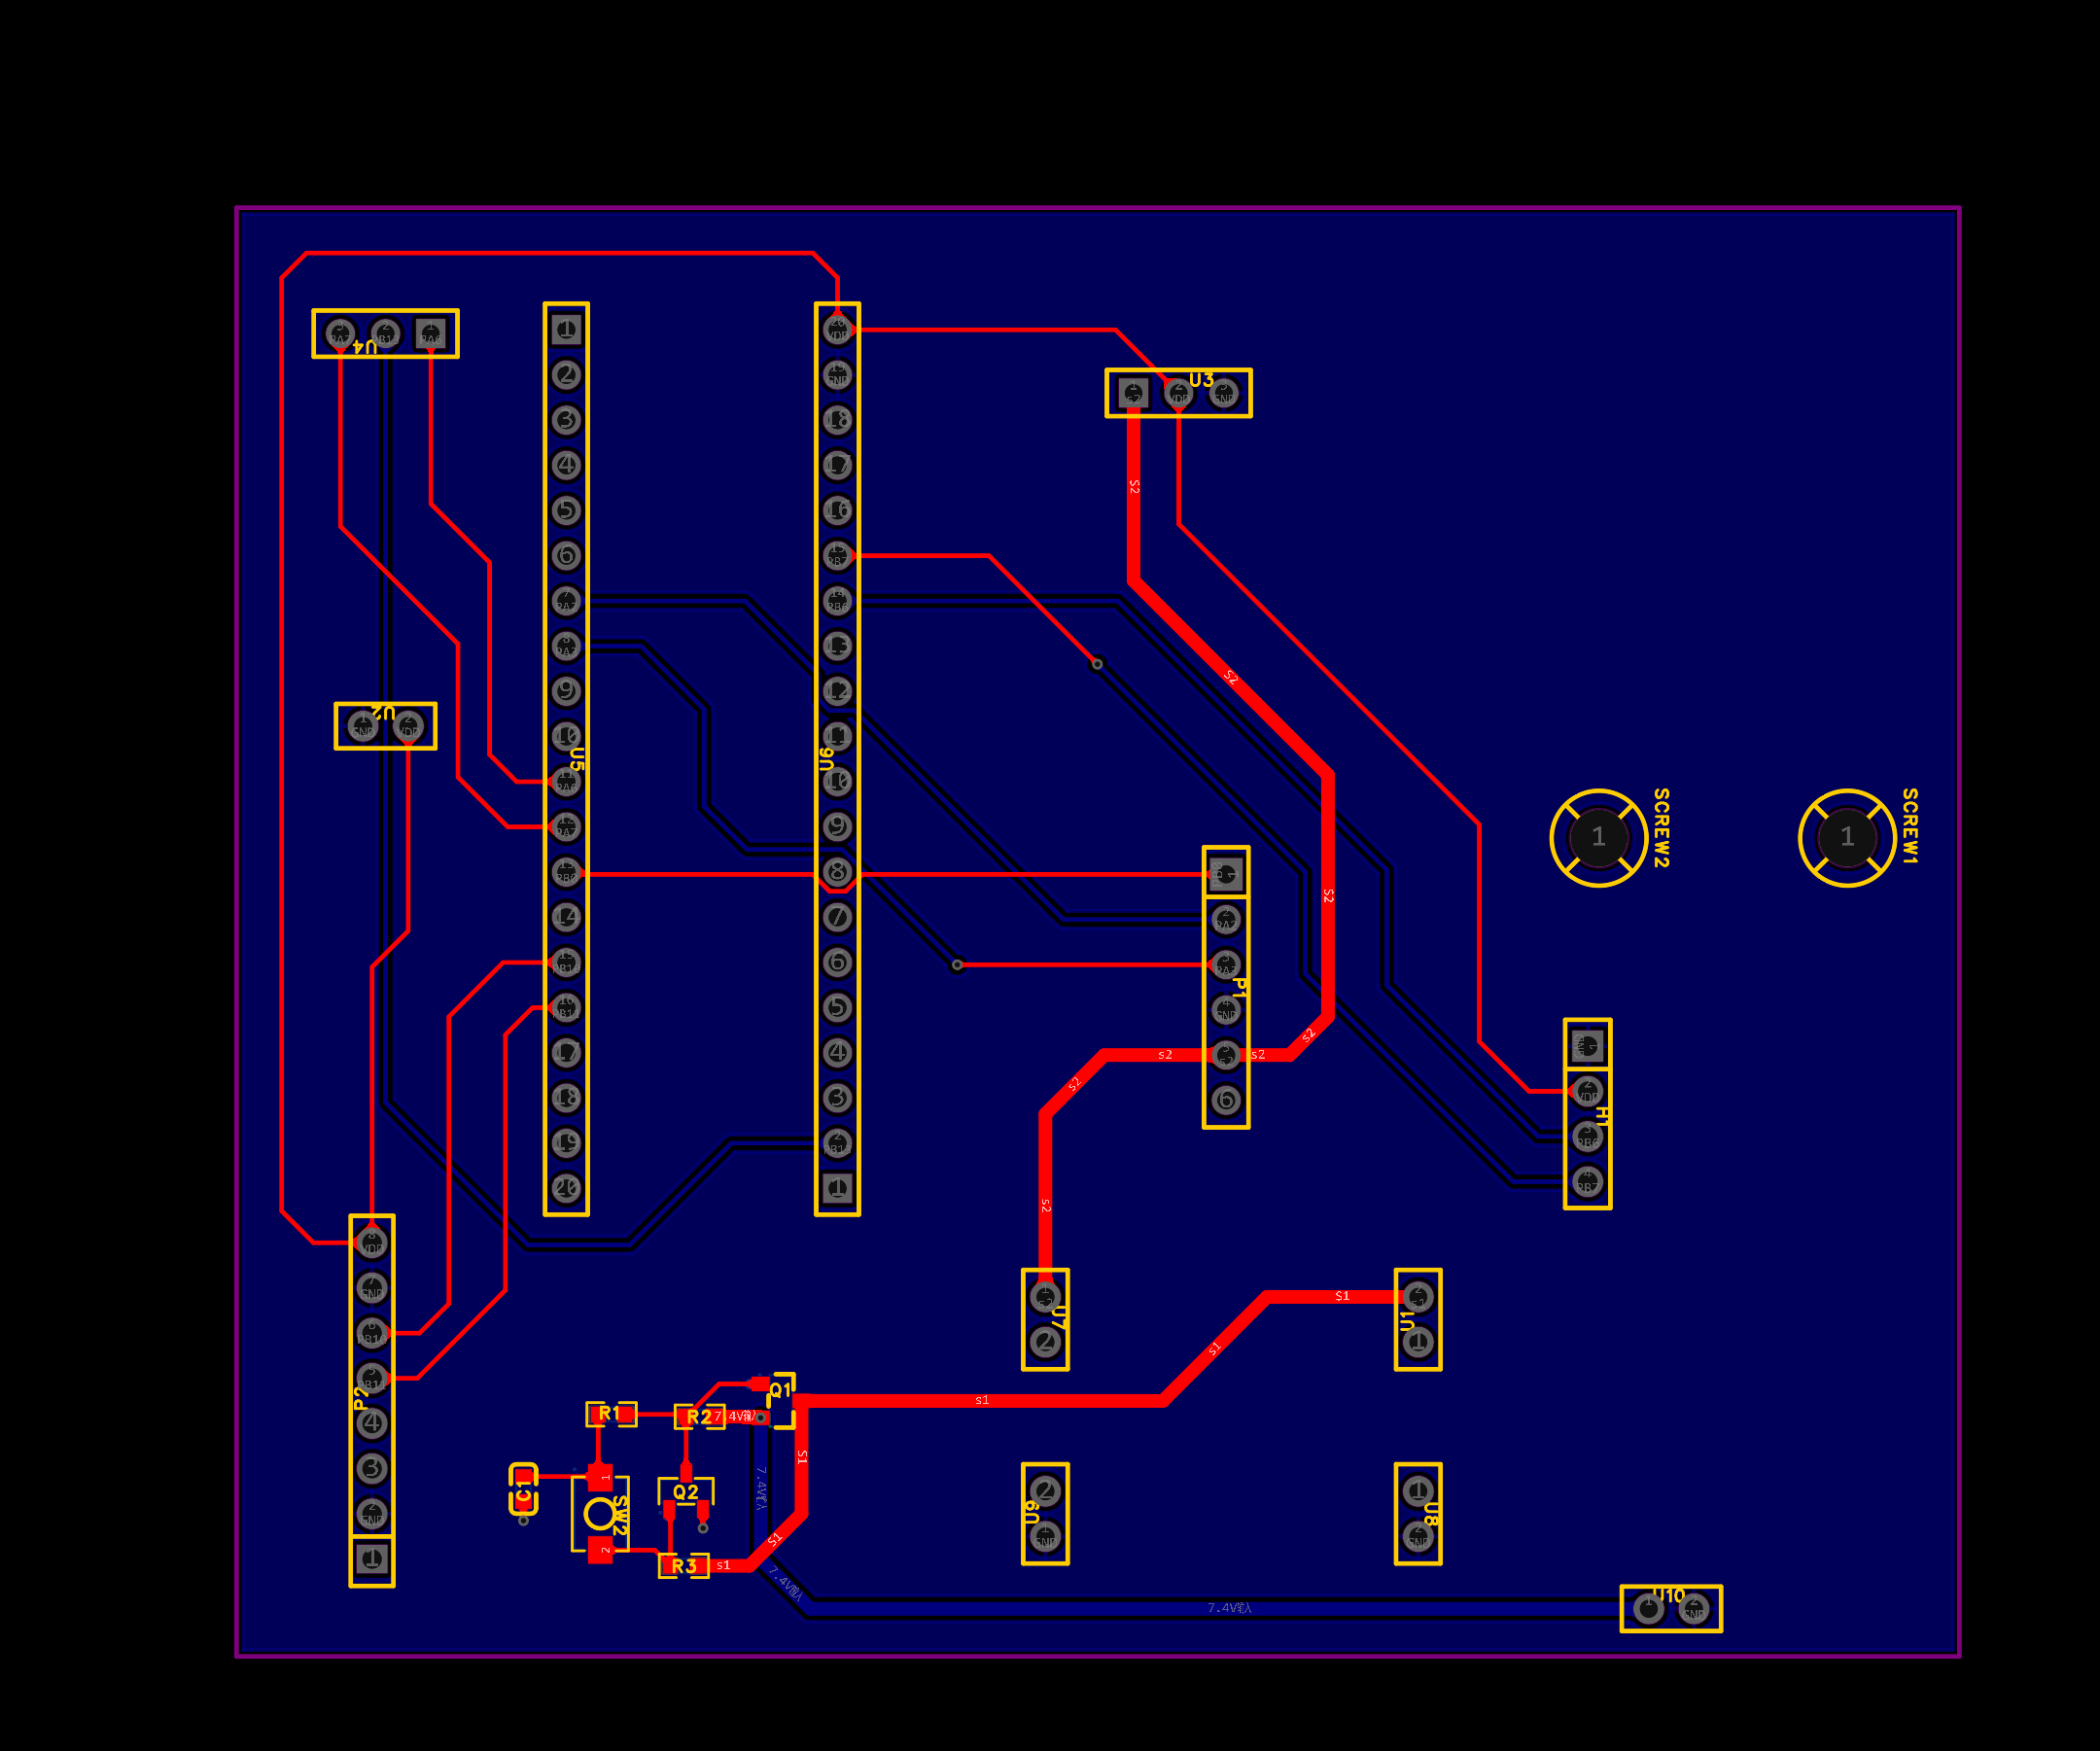
\includegraphics[width=0.9\textwidth]{figures/PCB终版.png}
    \caption{项目系统架构与功能模块总览（PCB终版布局，完整实现的硬件系统）}
    \label{fig:overview}
\end{figure}

\FloatBarrier
% !Mode:: "TeX:UTF-8"

\appendix
\section{\centering 设计图纸}

\subsection{系统总框图}
本智能手表系统以STM32F103C8T6为主控制器，通过I2C和USART总线连接三大外设模块，手机端通过蓝牙SPP协议与手表交互。系统完整原理图如图\ref{fig:ap_arch}所示。

\begin{figure}[h]
    \centering
    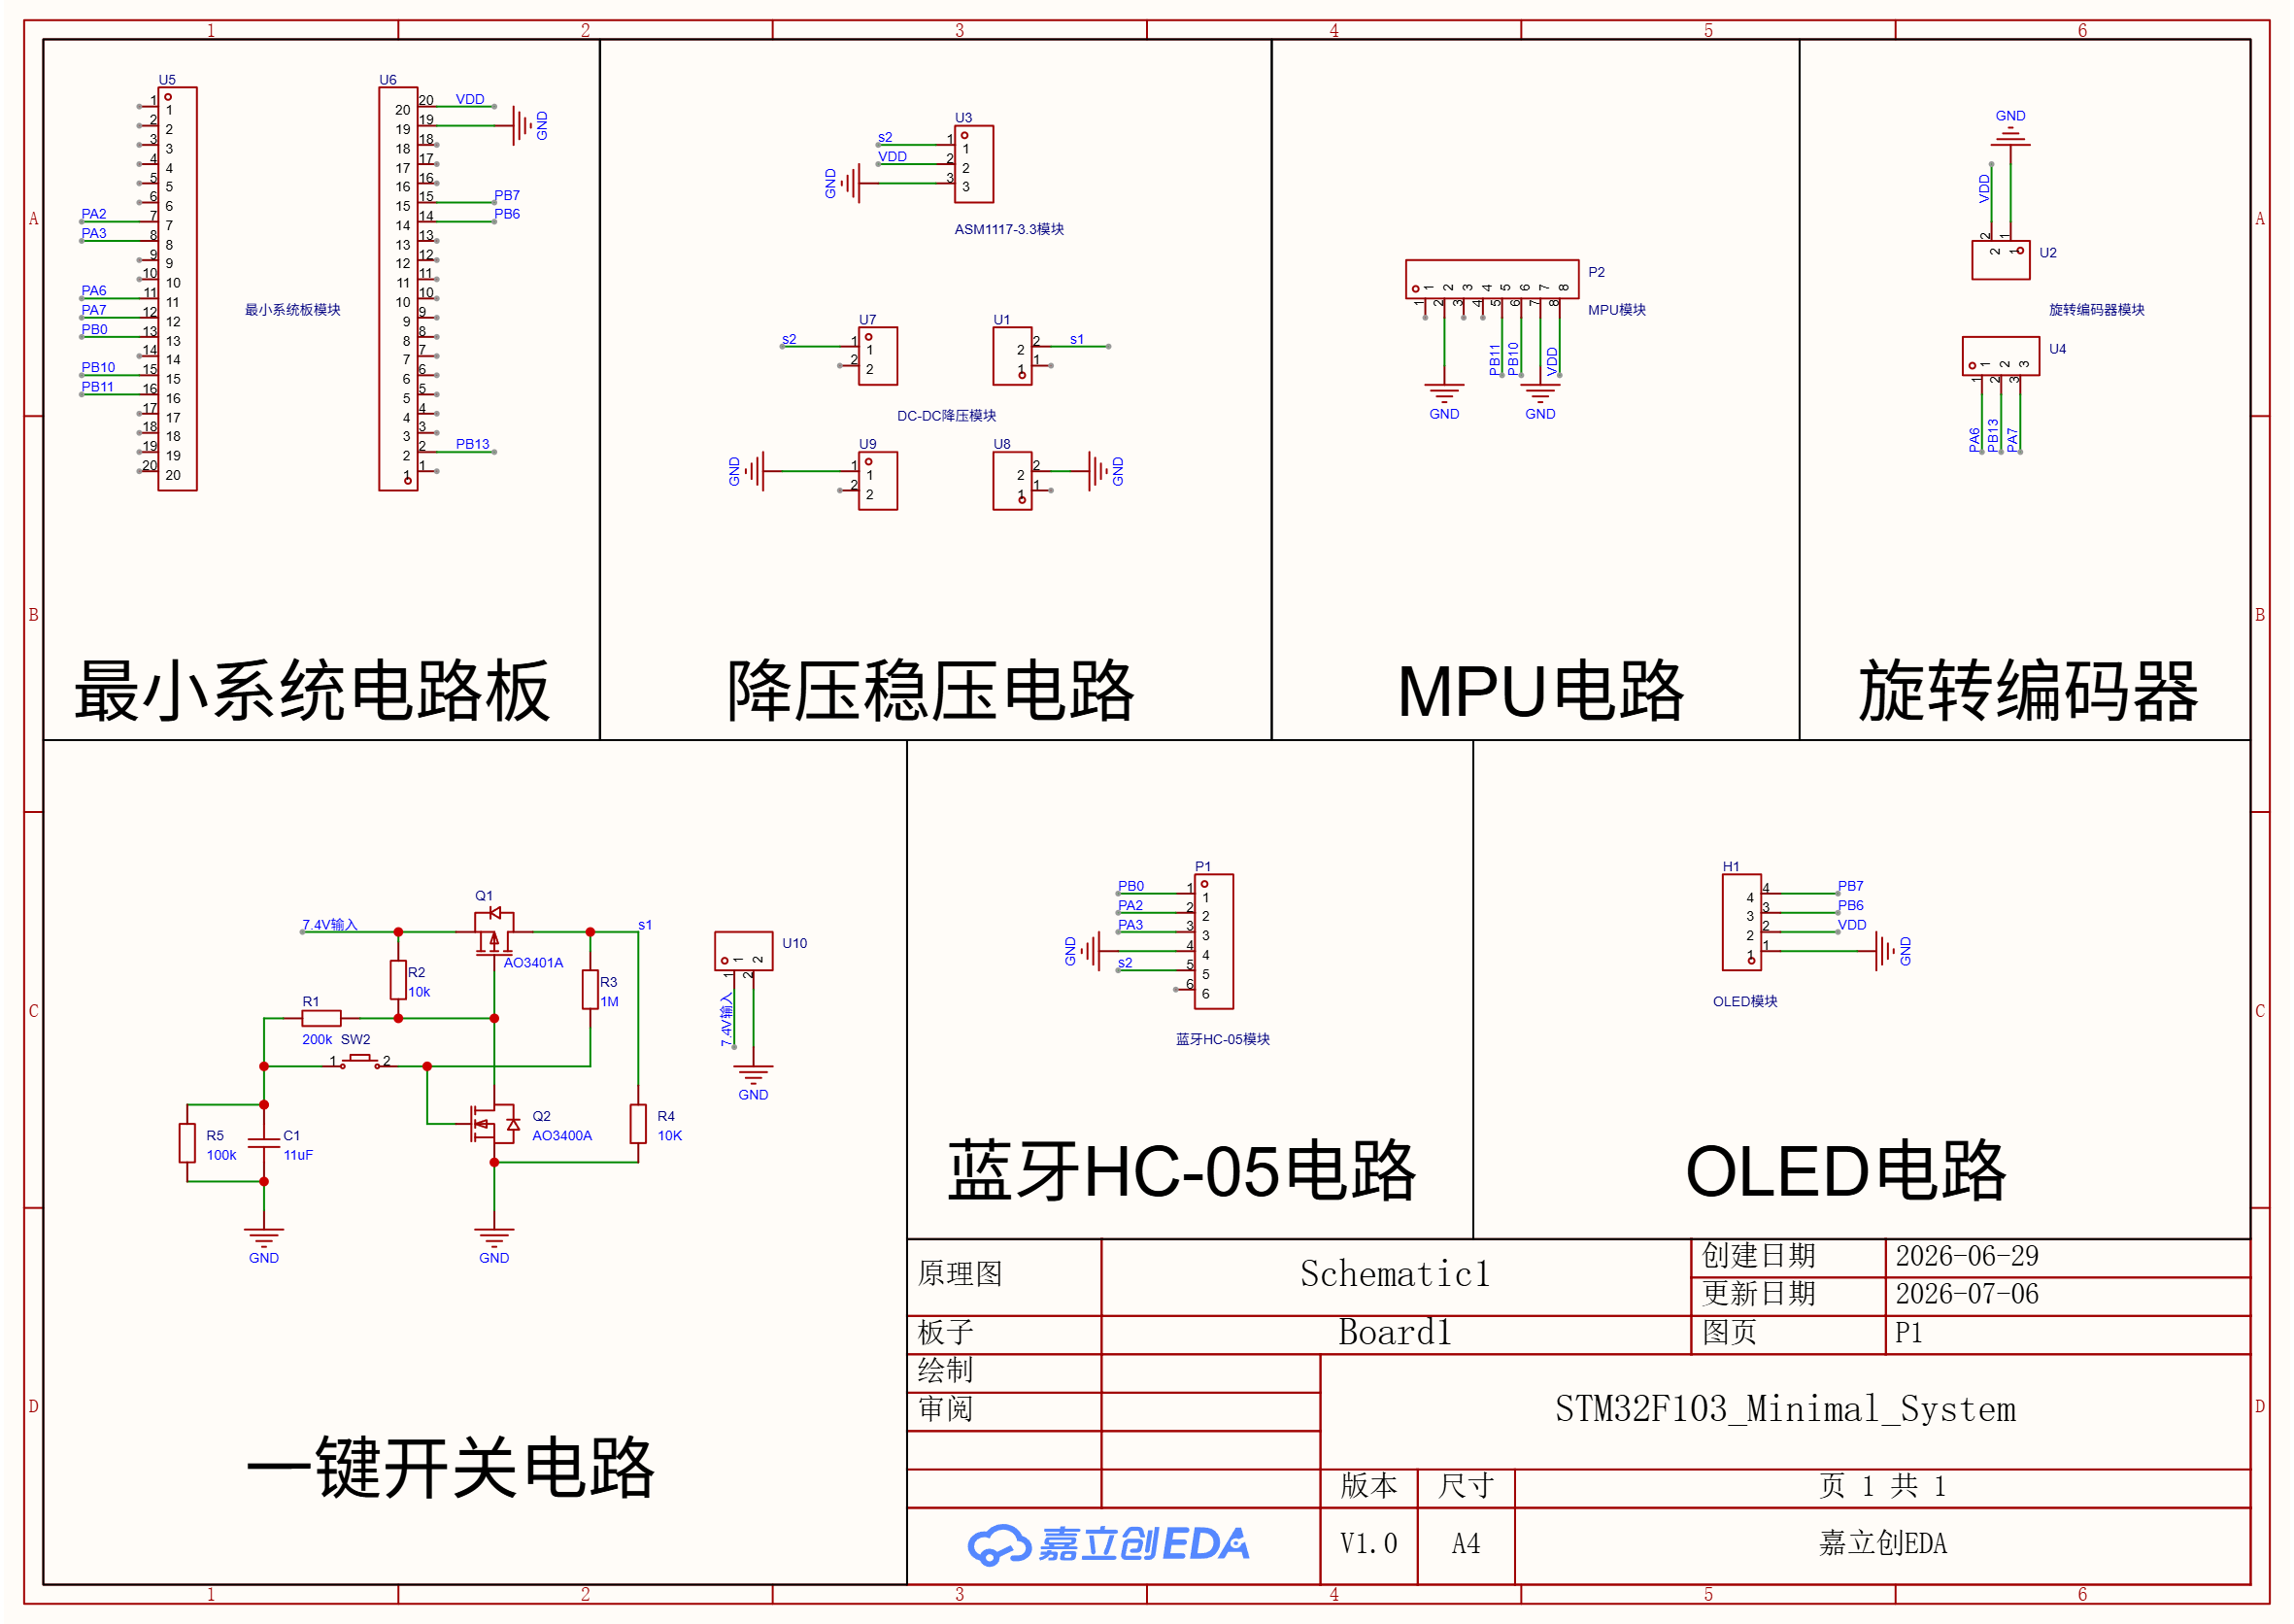
\includegraphics[width=0.95\textwidth]{figures/原理图终版.png}
    \caption{智能手表系统完整原理图（核心板 + 外设模块总线连接）}
    \label{fig:ap_arch}
\end{figure}

\FloatBarrier

\subsection{硬件引脚连接图}
各模块与STM32F103C8T6的引脚连接如表\ref{tab:ap_pinmap}所示，确保信号流向正确、电源与地分离设计。

\begin{table}[h]
    \centering
    \caption{硬件引脚连接表}
    \label{tab:ap_pinmap}
    \begin{tabular}{|l|l|l|l|}
        \hline
        \textbf{模块名称} & \textbf{模块引脚} & \textbf{STM32引脚} & \textbf{功能} \\ \hline
        SSD1306 OLED & VCC & 3.3V & 电源 \\ \hline
        SSD1306 OLED & GND & GND & 地 \\ \hline
        SSD1306 OLED & SCL & PB6 (I2C1\_SCL) & I2C时钟 \\ \hline
        SSD1306 OLED & SDA & PB7 (I2C1\_SDA) & I2C数据 \\ \hline
        MPU6050 & VCC & 3.3V & 电源 \\ \hline
        MPU6050 & GND & GND & 地 \\ \hline
        MPU6050 & SCL & PB10 (I2C2\_SCL) & I2C时钟 \\ \hline
        MPU6050 & SDA & PB11 (I2C2\_SDA) & I2C数据 \\ \hline
        HC-05蓝牙 & VCC & 5V & 电源 \\ \hline
        HC-05蓝牙 & GND & GND & 地 \\ \hline
        HC-05蓝牙 & TX & PA3 (USART2\_RX) & 模块发送→MCU接收 \\ \hline
        HC-05蓝牙 & RX & PA2 (USART2\_TX) & 模块接收←MCU发送 \\ \hline
        HC-05蓝牙 & STATE & PB0 (GPIO\_Input) & 连接状态检测 \\ \hline
        状态LED & Anode & PC13 & 运行状态指示 \\ \hline
        状态LED & Cathode & GND & 通过220$\Omega$电阻接地 \\ \hline
    \end{tabular}
\end{table}

\FloatBarrier

\subsection{软件模块调用关系}
固件软件采用分层模块化设计，主循环统一调度各功能模块。main.c作为调度中枢，调用驱动层和应用层各模块。模块间的调用关系如下：

\begin{itemize}
    \item \textbf{main.c（主循环调度器）} 直接调用以下模块的接口函数：
    \begin{itemize}
        \item oled.c — OLED显示驱动
        \item mpu6050.c — 六轴传感器驱动
        \item bluetooth.c — 蓝牙帧协议
        \item smartwatch\_ui.c — 多页面UI框架
        \item pedometer.c — 计步器算法
        \item soft\_rtc.c — 软RTC时钟
    \end{itemize}
    \item \textbf{所有功能模块} 均依赖 STM32 HAL驱动层（I2C1、I2C2、USART2、GPIO、TIM2、DMA）完成硬件交互
\end{itemize}

\FloatBarrier

\section{\centering 代码清单}

\subsection{STM32固件核心源文件}
固件源代码文件结构如表\ref{tab:ap_codefiles}所示，所有文件均位于工程Core目录下。

\begin{table}[h]
    \centering
    \caption{STM32固件源文件清单}
    \label{tab:ap_codefiles}
    \begin{tabular}{|l|l|r|l|}
        \hline
        \textbf{文件名} & \textbf{类型} & \textbf{行数} & \textbf{功能说明} \\ \hline
        main.c & 源文件 & 280 & 主循环、系统初始化、任务调度 \\ \hline
        oled.h / oled.c & 头/源文件 & 320 & SSD1306 OLED驱动与字模 \\ \hline
        mpu6050.h / mpu6050.c & 头/源文件 & 260 & MPU6050六轴传感器驱动 \\ \hline
        bluetooth.h / bluetooth.c & 头/源文件 & 220 & HC-05蓝牙帧协议实现 \\ \hline
        pedometer.h / pedometer.c & 头/源文件 & 180 & 计步器算法实现 \\ \hline
        smartwatch\_ui.h / smartwatch\_ui.c & 头/源文件 & 240 & OLED多页面UI框架 \\ \hline
        soft\_rtc.h / soft\_rtc.c & 头/源文件 & 120 & TIM2软RTC时钟实现 \\ \hline
        i2c\_drv.h / i2c\_drv.c & 头/源文件 & 80 & I2C总线恢复实现 \\ \hline
        gpio.c / usart.c / i2c.c / tim.c & 源文件 & 500 & STM32CubeMX生成的外设配置 \\ \hline
        stm32f1xx\_it.c & 源文件 & 150 & 中断服务函数（TIM2、USART2） \\ \hline
        \textbf{合计} & - & \textbf{2350} & - \\ \hline
    \end{tabular}
\end{table}

\FloatBarrier

\subsection{核心代码片段}

\subsubsection{OLED初始化代码（oled.c）}
\begin{lstlisting}[language=C, basicstyle=\ttfamily\footnotesize, numbers=left, numberstyle=\tiny, stepnumber=1, numbersep=5pt, frame=shadowbox, rulesepcolor=\color{red!20!green!20!blue!20}, keywordstyle=\color{blue}\bfseries, commentstyle=\color{codegreen}, stringstyle=\color{orange}, showstringspaces=false]
void OLED_Init(void)
{
    /* 1. 发送初始化命令序列 */
    OLED_Write_Cmd(0xAE); /* 关闭显示 */
    OLED_Write_Cmd(0x20); /* 设置内存寻址模式 */
    OLED_Write_Cmd(0x10); /* 页寻址模式 */
    OLED_Write_Cmd(0xB0); /* 设置页地址 */
    OLED_Write_Cmd(0xC8); /* COM输出扫描方向 */
    OLED_Write_Cmd(0x00); /* 设置低位列地址 */
    OLED_Write_Cmd(0x10); /* 设置高位列地址 */
    OLED_Write_Cmd(0x40); /* 设置起始行地址 */
    OLED_Write_Cmd(0x81); /* 设置对比度 */
    OLED_Write_Cmd(0xFF); /* 最大对比度 */
    OLED_Write_Cmd(0xA1); /* 段重映射 */
    OLED_Write_Cmd(0xA6); /* 正常显示模式 */
    OLED_Write_Cmd(0xA8); /* 设置多路复用率 */
    OLED_Write_Cmd(0x3F); /* 1/64 duty */
    OLED_Write_Cmd(0xA4); /* 全局显示开启 */
    OLED_Write_Cmd(0xD3); /* 设置显示偏移 */
    OLED_Write_Cmd(0x00); /* 无偏移 */
    OLED_Write_Cmd(0xD5); /* 设置时钟分频因子 */
    OLED_Write_Cmd(0xF0); /* 高频时钟 */
    OLED_Write_Cmd(0xD9); /* 设置预充电周期 */
    OLED_Write_Cmd(0x22); /* 标准预充电 */
    OLED_Write_Cmd(0xDA); /* 设置COM引脚配置 */
    OLED_Write_Cmd(0x12); /* 标准配置 */
    OLED_Write_Cmd(0xDB); /* 设置VCOMH */
    OLED_Write_Cmd(0x20); /* 0.77*VCC */
    OLED_Write_Cmd(0x8D); /* 电荷泵设置 */
    OLED_Write_Cmd(0x14); /* 启用电荷泵 */
    OLED_Write_Cmd(0xAF); /* 开启显示 */
    OLED_Clear(); /* 清屏 */
}
\end{lstlisting}

\subsubsection{MPU6050六轴数据读取代码（mpu6050.c）}
\begin{lstlisting}[language=C, basicstyle=\ttfamily\footnotesize, numbers=left, numberstyle=\tiny, stepnumber=1, numbersep=5pt, frame=shadowbox, rulesepcolor=\color{red!20!green!20!blue!20}, keywordstyle=\color{blue}\bfseries, commentstyle=\color{codegreen}, stringstyle=\color{orange}, showstringspaces=false]
void MPU6050_Read_Accel(float *ax, float *ay, float *az)
{
    uint8_t buf[6];
    int16_t raw_x, raw_y, raw_z;

    /* 从0x3B寄存器连续读取6字节加速度数据 */
    HAL_I2C_Mem_Read(&hi2c2, MPU6050_ADDR, 0x3B, 1, buf, 6, HAL_MAX_DELAY);

    /* 组合高低字节（大端格式，高字节在前） */
    raw_x = (int16_t)((buf[0] << 8) | buf[1]);
    raw_y = (int16_t)((buf[2] << 8) | buf[3]);
    raw_z = (int16_t)((buf[4] << 8) | buf[5]);

    /* 转换为物理量（加速度量程±2g，灵敏度16384 LSB/g） */
    *ax = (float)raw_x / 16384.0f * 9.8f;  /* m/s^2 */
    *ay = (float)raw_y / 16384.0f * 9.8f;
    *az = (float)raw_z / 16384.0f * 9.8f;
}

void MPU6050_Read_Gyro(float *gx, float *gy, float *gz)
{
    uint8_t buf[6];
    int16_t raw_x, raw_y, raw_z;

    /* 从0x43寄存器连续读取6字节陀螺仪数据 */
    HAL_I2C_Mem_Read(&hi2c2, MPU6050_ADDR, 0x43, 1, buf, 6, HAL_MAX_DELAY);

    raw_x = (int16_t)((buf[0] << 8) | buf[1]);
    raw_y = (int16_t)((buf[2] << 8) | buf[3]);
    raw_z = (int16_t)((buf[4] << 8) | buf[5]);

    /* 转换为物理量（陀螺仪量程±250°/s，灵敏度131 LSB/°/s） */
    *gx = (float)raw_x / 131.0f;  /* deg/s */
    *gy = (float)raw_y / 131.0f;
    *gz = (float)raw_z / 131.0f;
}
\end{lstlisting}

\subsubsection{蓝牙帧协议发送代码（bluetooth.c）}
\begin{lstlisting}[language=C, basicstyle=\ttfamily\footnotesize, numbers=left, numberstyle=\tiny, stepnumber=1, numbersep=5pt, frame=shadowbox, rulesepcolor=\color{red!20!green!20!blue!20}, keywordstyle=\color{blue}\bfseries, commentstyle=\color{codegreen}, stringstyle=\color{orange}, showstringspaces=false]
void Bluetooth_Send_Frame(uint8_t cmd, uint8_t *data, uint16_t len)
{
    uint8_t frame[256];
    uint8_t checksum = 0;
    uint16_t idx = 0;
    uint16_t i;

    /* 1. 组装帧格式：STX(0xAA) + CMD + DATA + CHK(XOR) + ETX(0x55) */
    frame[idx++] = 0xAA;          /* 帧头 */
    frame[idx++] = cmd;           /* 命令字节 */

    /* 2. 填充数据载荷 */
    for (i = 0; i < len; i++)
    {
        frame[idx++] = data[i];
    }

    /* 3. 计算XOR校验（对CMD和DATA所有字节做异或） */
    checksum = cmd;
    for (i = 0; i < len; i++)
    {
        checksum ^= data[i];
    }
    frame[idx++] = checksum;     /* 校验字节 */
    frame[idx++] = 0x55;         /* 帧尾 */

    /* 4. 通过USART2发送完整帧（阻塞方式） */
    HAL_UART_Transmit(&huart2, frame, idx, HAL_MAX_DELAY);
}
\end{lstlisting}

\subsubsection{计步器算法核心代码（pedometer.c）}
\begin{lstlisting}[language=C, basicstyle=\ttfamily\footnotesize, numbers=left, numberstyle=\tiny, stepnumber=1, numbersep=5pt, frame=shadowbox, rulesepcolor=\color{red!20!green!20!blue!20}, keywordstyle=\color{blue}\bfseries, commentstyle=\color{codegreen}, stringstyle=\color{orange}, showstringspaces=false]
static float filtered_mag = 1.0f;      /* 低通滤波输出 */
static float mag_max = 1.3f;           /* 动态最大值 */
static float mag_min = 0.7f;           /* 动态最小值 */
static uint32_t last_step_tick = 0;    /* 上一步时间戳 */
static uint32_t step_count = 0;        /* 总步数 */

uint8_t Pedometer_Update(float ax, float ay, float az)
{
    /* 1. 计算加速度向量幅值（单位: g） */
    float mag = sqrtf(ax * ax + ay * ay + az * az) / 9.8f;

    /* 2. 一阶低通滤波（指数加权平均，α=0.7） */
    filtered_mag = 0.7f * filtered_mag + 0.3f * mag;

    /* 3. 更新滑动窗口内的最大最小值（动态阈值） */
    if (filtered_mag > mag_max) mag_max = filtered_mag;
    if (filtered_mag < mag_min) mag_min = filtered_mag;

    /* 4. 计算当前阈值（中点+偏移量） */
    float threshold = (mag_max + mag_min) * 0.5f + 0.05f;

    /* 5. 峰值检测：从低于阈值上升到高于阈值时标记为一步 */
    static uint8_t below_threshold = 1;
    uint32_t now = HAL_GetTick();
    uint8_t new_step = 0;

    if (filtered_mag < threshold)
    {
        below_threshold = 1;
    }
    else if (below_threshold && (now - last_step_tick) > 200)
    {
        /* 上升沿 + 200ms最小步间间隔 = 确认一步 */
        step_count++;
        last_step_tick = now;
        below_threshold = 0;
        new_step = 1;
    }

    /* 6. 定期重置动态阈值窗口（约每4秒） */
    static uint32_t window_reset = 0;
    if ((now - window_reset) > 4000)
    {
        mag_max = filtered_mag + 0.1f;
        mag_min = filtered_mag - 0.1f;
        window_reset = now;
    }

    return new_step;
}
\end{lstlisting}

\subsubsection{软RTC中断代码（soft\_rtc.c）}
\begin{lstlisting}[language=C, basicstyle=\ttfamily\footnotesize, numbers=left, numberstyle=\tiny, stepnumber=1, numbersep=5pt, frame=shadowbox, rulesepcolor=\color{red!20!green!20!blue!20}, keywordstyle=\color{blue}\bfseries, commentstyle=\color{codegreen}, stringstyle=\color{orange}, showstringspaces=false]
static uint8_t hour = 0, minute = 0, second = 0;
static uint8_t day = 1, month = 1;
static uint16_t year = 2025;

/* TIM2 1Hz中断服务回调（在stm32f1xx_it.c中调用） */
void Soft_RTC_Handler(void)
{
    second++;
    if (second >= 60)
    {
        second = 0;
        minute++;
        if (minute >= 60)
        {
            minute = 0;
            hour++;
            if (hour >= 24)
            {
                hour = 0;
                day++;
                /* 简化的月份天数处理（暂不考虑闰年2月） */
                uint8_t days_in_month[] = {31,28,31,30,31,30,31,31,30,31,30,31};
                if (day > days_in_month[month - 1])
                {
                    day = 1;
                    month++;
                    if (month > 12)
                    {
                        month = 1;
                        year++;
                    }
                }
            }
        }
    }
}

/* 蓝牙时间同步命令(0x02)处理：更新RTC */
void Soft_RTC_Set_Time(uint8_t h, uint8_t m, uint8_t s)
{
    if (h < 24) hour = h;
    if (m < 60) minute = m;
    if (s < 60) second = s;
}
\end{lstlisting}

\subsubsection{Android端蓝牙协议解析代码（BtProtocol.kt）}
\begin{lstlisting}[language=Kotlin, basicstyle=\ttfamily\footnotesize, numbers=left, numberstyle=\tiny, stepnumber=1, numbersep=5pt, frame=shadowbox, rulesepcolor=\color{red!20!green!20!blue!20}, keywordstyle=\color{blue}\bfseries, commentstyle=\color{codegreen}, stringstyle=\color{orange}, showstringspaces=false]
object BtProtocol {
    const val STX = 0xAA.toByte()  /* 帧头 */
    const val ETX = 0x55.toByte()  /* 帧尾 */
    const val CMD_SENSOR = 0x01.toByte()  /* 传感器数据 */
    const val CMD_TIME = 0x02.toByte()    /* 时间同步 */
    const val CMD_STEP = 0x03.toByte()    /* 计步数据 */

    /* 解析手表上报的传感器数据帧（24字节：6个float） */
    fun parseSensorData(data: ByteArray): FloatArray {
        val values = FloatArray(6)
        /* 小端格式：每个float占4字节 */
        val buffer = ByteBuffer.wrap(data).order(ByteOrder.LITTLE_ENDIAN)
        for (i in 0 until 6) {
            values[i] = buffer.float
        }
        /* values: ax, ay, az(加速度m/s^2), gx, gy, gz(陀螺仪deg/s) */
        return values
    }

    /* 组装时间同步命令下发给手表 */
    fun buildTimeSyncFrame(hour: Int, minute: Int, second: Int): ByteArray {
        val frame = ByteArray(6)
        frame[0] = STX
        frame[1] = CMD_TIME
        frame[2] = hour.toByte()
        frame[3] = minute.toByte()
        frame[4] = second.toByte()
        /* XOR校验 */
        frame[5] = (CMD_TIME.toInt() xor hour xor minute xor second).toByte()
        /* 注意：实际帧长度还需追加ETX */
        return frame + byteArrayOf(ETX)
    }
}
\end{lstlisting}

\section{\centering 参考文献}

\addcontentsline{toc}{section}{参考文献}

\begin{thebibliography}{99}

\bibitem{ref1} 刘火良，杨森. \textit{STM32库开发实战指南：基于野火STM32全系列开发板}. 机械工业出版社, 2020.

\bibitem{ref2} STMicroelectronics. \textit{STM32F103xC, STM32F103xD, STM32F103xE Reference Manual} (RM0008). Rev 21, 2023.

\bibitem{ref3} STMicroelectronics. \textit{PM0056 Programming Manual: STM32F10xxx Cortex-M3 Programming}. Rev 5, 2020.

\bibitem{ref4} Solomon Systech. \textit{SSD1306 128x64 Dot Matrix OLED/PLED Segment/Common Driver with Controller Data Sheet}. Rev 1.1, 2008.

\bibitem{ref5} TDK InvenSense. \textit{MPU-6000 and MPU-6050 Product Specification Register Map and Descriptions}. Rev 4.2, 2013.

\bibitem{ref6} HC-05 Bluetooth Module. \textit{HC-05 Product Data Sheet}. Guangzhou HC Intelligent Technology Co., Ltd.

\bibitem{ref7} Carmine Noviello. \textit{Mastering STM32} (2nd ed.). Leanpub, 2022.

\bibitem{ref8} Joseph Yiu. \textit{The Definitive Guide to ARM Cortex-M3 and Cortex-M4 Processors} (3rd ed.). Newnes, 2013.

\bibitem{ref9} 王忠飞，严冬. \textit{嵌入式系统原理及应用——基于ARM Cortex-M3内核的STM32微控制器}. 清华大学出版社, 2019.

\bibitem{ref10} Lars Bengtsson. \textit{Step Counter Using Accelerometer Data}. Technical Report, University of Gothenburg, 2019.

\bibitem{ref11} Philip Alpay. \textit{Programming Android with Kotlin: Achieving Structured Concurrency with Coroutines}. O'Reilly Media, 2021.

\bibitem{ref12} Google. \textit{Android Developers: Bluetooth Overview}. https://developer.android.com/guide/topics/connectivity/bluetooth, 2024.

\end{thebibliography}


\end{document}